         \chapter{Quantitative aspects of chemical change}
    \setcounter{figure}{1}
    \setcounter{subfigure}{1}
    \label{0044f0dab6cfd2ca2bac282dc4009886}
    
    
    
    
       
         \section{ Moles and molar mass}
    \nopagebreak
            \label{m38717} $ \hspace{-5pt}\begin{array}{cccccccccccc}   
\includegraphics[width=0.75cm]{col11305.imgs/summary_fullmarks.png} &   
\includegraphics[width=0.75cm]{col11305.imgs/summary_video.png} &   \end{array} $ \hspace{2 pt}\raisebox{-5 pt}{} {(section shortcode: P10084 )} \par 
    
    
    
    
    
    
  
    \label{m38717*cid1}
            \subsection{ Quantitative Aspects of Chemical Change}
            \nopagebreak
            
      
      \label{m38717*id275167}An equation for a chemical reaction can provide us with a lot of useful information. It tells us what the reactants and the products are in the reaction, and it also tells us the ratio in which the reactants combine to form products. Look at the equation below:\par 
      \label{m38717*id275172}
        \begin{math}Fe+\mathrm{S}\to \mathrm{FeS}\end{math}
      \par 
      
      \label{m38717*id275542}In this reaction, every atom of iron (\begin{math}Fe\end{math}) will react with a single atom of sulphur (\begin{math}\mathrm{S}\end{math}) to form one molecule of iron sulphide (\begin{math}\mathrm{FeS}\end{math}). However, what the equation doesn't tell us, is the \textbf{quantities} or the \textbf{amount} of each substance that is involved. You may for example be given a small sample of iron for the reaction. How will you know how many atoms of iron are in this sample? And how many atoms of sulphur will you need for the reaction to use up all the iron you have? Is there a way of knowing what mass of iron sulphide will be produced at the end of the reaction? These are all very important questions, especially when the reaction is an industrial one, where it is important to know the quantities of reactants that are needed, and the quantity of product that will be formed. This chapter will look at how to quantify the changes that take place in chemical reactions.\par 
    
    \label{m38717*cid2}
            \subsection{ The Mole}
            \nopagebreak
            
      
      \label{m38717*id275573}Sometimes it is important to know exactly how many particles (e.g. atoms or molecules) are in a sample of a substance, or what quantity of a substance is needed for a chemical reaction to take place.\par 
      
      
      
      
      
\label{m38717*eip-872}The amount of substance is so important in chemistry that it is given it's own name, which is the mole.  \par \label{m38717*fhsst!!!underscore!!!id119}\begin{definition}
	  \begin{tabular*}{15 cm}{m{15 mm}m{}}
	\hspace*{-50pt}  
\includegraphics[width=0.5in]{col11305.imgs/psflag2.png}   & \Definition{   \label{id2496528}\textbf{ Mole }} { \label{m38717*meaningfhsst!!!underscore!!!id119}
      \label{m38717*id275969}The mole (abbreviation 'n') is the SI (Standard International) unit for 'amount of substance'. \par 
       } 
      \end{tabular*}
      \end{definition}

      
\label{m38717*eip-392}Now that we know what a mole is, we can relate it to something that we know already. This is the relative atomic mass. For example, if we have a sample containing 1g of hydrogen then we have 1 mole of hydrogen, since the relative atomic mass of hydrogen is 1u.\par \label{m38717*eip-503}We can build up to the idea of Avogadro's number. For example, if you have 12 eggs then you have a dozen eggs. After this number we get a gross of eggs, which is 144 eggs. Finally if we wanted one mole of eggs this would be \begin{math}6,022\ensuremath{\times}{10}^{23}\end{math}. That is a lot of eggs!\par \label{m38717*eip-460}In one mole of any substance, there are \begin{math}6,022\ensuremath{\times}{10}^{23}\end{math} particles. When we talk about the mole, we should always say what the particles are. The particles can be atoms, molecules, electrons, or almost anything else.\par \label{m38717*fhsst!!!underscore!!!id123}\begin{definition}
	  \begin{tabular*}{15 cm}{m{15 mm}m{}}
	\hspace*{-50pt}  
\includegraphics[width=0.5in]{col11305.imgs/psflag2.png}   & \Definition{   \label{id2496617}\textbf{ Avogadro's number }} { \label{m38717*meaningfhsst!!!underscore!!!id123}
      \label{m38717*id276010}The number of particles in a mole, equal to \begin{math}6,022\ensuremath{\times}{10}^{23}\end{math}. \par 
       } 
      \end{tabular*}
      \end{definition}

\label{m38717*eip-446}If we were to write out Avogadro's number then it would look like:
\begin{math}602\phantom{\rule{1pt}{0ex}}200\phantom{\rule{1pt}{0ex}}000\phantom{\rule{1pt}{0ex}}000\phantom{\rule{1pt}{0ex}}000\phantom{\rule{1pt}{0ex}}000\phantom{\rule{1pt}{0ex}}000\phantom{\rule{1pt}{0ex}}000\end{math}. This is a very large number. If we had this number of cold drink cans, then we could cover the surface of the earth to a depth of over \begin{math}300\phantom{\rule{2pt}{0ex}}\mathrm{km}\end{math}! If you could count atoms at a rate of 10 million per second, then it would take you 2 billion years to count the atoms in one mole!\par \label{m38717*notfhsst!!!underscore!!!id126}
\begin{tabular}{cc}
	\hspace*{-50pt}\raisebox{-8 mm}{\hspace{-0.2in}
\includegraphics[width=0.75in]{col11305.imgs/psfact2.png} } & 

	\begin{minipage}{0.85\textwidth}
	\begin{note}
      {note: } The original hypothesis that was proposed by Amadeo Avogadro was that \textsl{'equal volumes of gases, at the same temperature and pressure, contain the same number of molecules'}. His ideas were not accepted by the scientific community and it was only four years after his death, that his original hypothesis was accepted and that it became known as 'Avogadro's Law'. In honour of his contribution to science, the number of particles in one mole was named \textsl{Avogadro's number}.
	\end{note}
	\end{minipage}
	\end{tabular}
	\par
      
\label{m38717*secfhsst!!!underscore!!!id127}
            \subsubsection{  Moles and mass
      }
            \nopagebreak
            
      \label{m38717*id276067}\begin{enumerate}[noitemsep, label=\textbf{\arabic*}. ] 
            \label{m38717*uid2}\item 
Complete the following table:

    % \textbf{m38717*id276082}\par
    
    % how many colspecs?  4
          % name: cnx:colspec
            % colnum: 1
            % colwidth: 10*
            % latex-name: columna
            % colname: 
            % align/tgroup-align/default: //left
            % -------------------------
            % name: cnx:colspec
            % colnum: 2
            % colwidth: 10*
            % latex-name: columnb
            % colname: 
            % align/tgroup-align/default: //left
            % -------------------------
            % name: cnx:colspec
            % colnum: 3
            % colwidth: 10*
            % latex-name: columnc
            % colname: 
            % align/tgroup-align/default: //left
            % -------------------------
            % name: cnx:colspec
            % colnum: 4
            % colwidth: 10*
            % latex-name: columnd
            % colname: 
            % align/tgroup-align/default: //left
            % -------------------------
      
    
    \setlength\mytablespace{8\tabcolsep}
    \addtolength\mytablespace{5\arrayrulewidth}
    \setlength\mytablewidth{\linewidth}
        
    
    \setlength\mytableroom{\mytablewidth}
    \addtolength\mytableroom{-\mytablespace}
    
    \setlength\myfixedwidth{0pt}
    \setlength\mystarwidth{\mytableroom}
        \addtolength\mystarwidth{-\myfixedwidth}
        \divide\mystarwidth 40
        
    
      % ----- Begin capturing width of table in LR mode woof
      \settowidth{\mytableboxwidth}{\begin{tabular}[t]{|l|l|l|l|}\hline
    % count in rowspan-info-nodeset: 4
    % align/colidx: left,1
    
    % rowcount: '0' | start: 'false' | colidx: '1'
    
        % Formatting a regular cell and recurring on the next sibling
        \textbf{Element} &
      % align/colidx: left,2
    
    % rowcount: '0' | start: 'false' | colidx: '2'
    
        % Formatting a regular cell and recurring on the next sibling
        \textbf{Relative atomic mass (u)} &
      % align/colidx: left,3
    
    % rowcount: '0' | start: 'false' | colidx: '3'
    
        % Formatting a regular cell and recurring on the next sibling
        \textbf{Sample mass (g)} &
      % align/colidx: left,4
    
    % rowcount: '0' | start: 'false' | colidx: '4'
    
        % Formatting a regular cell and recurring on the next sibling
        \textbf{Number of moles in the sample}% make-rowspan-placeholders
    % rowspan info: col1 '0' | 'false' | '' || col2 '0' | 'false' | '' || col3 '0' | 'false' | '' || col4 '0' | 'false' | ''
     \tabularnewline\cline{1-1}\cline{2-2}\cline{3-3}\cline{4-4}
      %--------------------------------------------------------------------
    % align/colidx: left,1
    
    % rowcount: '0' | start: 'false' | colidx: '1'
    
        % Formatting a regular cell and recurring on the next sibling
        Hydrogen &
      % align/colidx: left,2
    
    % rowcount: '0' | start: 'false' | colidx: '2'
    
        % Formatting a regular cell and recurring on the next sibling
        1.01 &
      % align/colidx: left,3
    
    % rowcount: '0' | start: 'false' | colidx: '3'
    
        % Formatting a regular cell and recurring on the next sibling
        1.01 &
      % align/colidx: left,4
    
    % rowcount: '0' | start: 'false' | colidx: '4'
    
        % Formatting a regular cell and recurring on the next sibling
        % make-rowspan-placeholders
    % rowspan info: col1 '0' | 'false' | '' || col2 '0' | 'false' | '' || col3 '0' | 'false' | '' || col4 '0' | 'false' | ''
     \tabularnewline\cline{1-1}\cline{2-2}\cline{3-3}\cline{4-4}
      %--------------------------------------------------------------------
    % align/colidx: left,1
    
    % rowcount: '0' | start: 'false' | colidx: '1'
    
        % Formatting a regular cell and recurring on the next sibling
        Magnesium &
      % align/colidx: left,2
    
    % rowcount: '0' | start: 'false' | colidx: '2'
    
        % Formatting a regular cell and recurring on the next sibling
        24.31 &
      % align/colidx: left,3
    
    % rowcount: '0' | start: 'false' | colidx: '3'
    
        % Formatting a regular cell and recurring on the next sibling
        24.31 &
      % align/colidx: left,4
    
    % rowcount: '0' | start: 'false' | colidx: '4'
    
        % Formatting a regular cell and recurring on the next sibling
        % make-rowspan-placeholders
    % rowspan info: col1 '0' | 'false' | '' || col2 '0' | 'false' | '' || col3 '0' | 'false' | '' || col4 '0' | 'false' | ''
     \tabularnewline\cline{1-1}\cline{2-2}\cline{3-3}\cline{4-4}
      %--------------------------------------------------------------------
    % align/colidx: left,1
    
    % rowcount: '0' | start: 'false' | colidx: '1'
    
        % Formatting a regular cell and recurring on the next sibling
        Carbon &
      % align/colidx: left,2
    
    % rowcount: '0' | start: 'false' | colidx: '2'
    
        % Formatting a regular cell and recurring on the next sibling
        12.01 &
      % align/colidx: left,3
    
    % rowcount: '0' | start: 'false' | colidx: '3'
    
        % Formatting a regular cell and recurring on the next sibling
        24.02 &
      % align/colidx: left,4
    
    % rowcount: '0' | start: 'false' | colidx: '4'
    
        % Formatting a regular cell and recurring on the next sibling
        % make-rowspan-placeholders
    % rowspan info: col1 '0' | 'false' | '' || col2 '0' | 'false' | '' || col3 '0' | 'false' | '' || col4 '0' | 'false' | ''
     \tabularnewline\cline{1-1}\cline{2-2}\cline{3-3}\cline{4-4}
      %--------------------------------------------------------------------
    % align/colidx: left,1
    
    % rowcount: '0' | start: 'false' | colidx: '1'
    
        % Formatting a regular cell and recurring on the next sibling
        Chlorine &
      % align/colidx: left,2
    
    % rowcount: '0' | start: 'false' | colidx: '2'
    
        % Formatting a regular cell and recurring on the next sibling
        35.45 &
      % align/colidx: left,3
    
    % rowcount: '0' | start: 'false' | colidx: '3'
    
        % Formatting a regular cell and recurring on the next sibling
        70.9 &
      % align/colidx: left,4
    
    % rowcount: '0' | start: 'false' | colidx: '4'
    
        % Formatting a regular cell and recurring on the next sibling
        % make-rowspan-placeholders
    % rowspan info: col1 '0' | 'false' | '' || col2 '0' | 'false' | '' || col3 '0' | 'false' | '' || col4 '0' | 'false' | ''
     \tabularnewline\cline{1-1}\cline{2-2}\cline{3-3}\cline{4-4}
      %--------------------------------------------------------------------
    % align/colidx: left,1
    
    % rowcount: '0' | start: 'false' | colidx: '1'
    
        % Formatting a regular cell and recurring on the next sibling
        Nitrogen &
      % align/colidx: left,2
    
    % rowcount: '0' | start: 'false' | colidx: '2'
    
        % Formatting a regular cell and recurring on the next sibling
         &
      % align/colidx: left,3
    
    % rowcount: '0' | start: 'false' | colidx: '3'
    
        % Formatting a regular cell and recurring on the next sibling
        42.08 &
      % align/colidx: left,4
    
    % rowcount: '0' | start: 'false' | colidx: '4'
    
        % Formatting a regular cell and recurring on the next sibling
        % make-rowspan-placeholders
    % rowspan info: col1 '0' | 'false' | '' || col2 '0' | 'false' | '' || col3 '0' | 'false' | '' || col4 '0' | 'false' | ''
     \tabularnewline\cline{1-1}\cline{2-2}\cline{3-3}\cline{4-4}
      %--------------------------------------------------------------------
    \end{tabular}} % end mytableboxwidth set
      \addtocounter{footnote}{-0}
      
      % ----- End capturing width of table in LR mode
    
        % ----- LR or paragraph mode: must test
        % ----- Begin capturing height of table
        \settoheight{\mytableboxheight}{\begin{tabular}[t]{|l|l|l|l|}\hline
    % count in rowspan-info-nodeset: 4
    % align/colidx: left,1
    
    % rowcount: '0' | start: 'false' | colidx: '1'
    
        % Formatting a regular cell and recurring on the next sibling
        \textbf{Element} &
      % align/colidx: left,2
    
    % rowcount: '0' | start: 'false' | colidx: '2'
    
        % Formatting a regular cell and recurring on the next sibling
        \textbf{Relative atomic mass (u)} &
      % align/colidx: left,3
    
    % rowcount: '0' | start: 'false' | colidx: '3'
    
        % Formatting a regular cell and recurring on the next sibling
        \textbf{Sample mass (g)} &
      % align/colidx: left,4
    
    % rowcount: '0' | start: 'false' | colidx: '4'
    
        % Formatting a regular cell and recurring on the next sibling
        \textbf{Number of moles in the sample}% make-rowspan-placeholders
    % rowspan info: col1 '0' | 'false' | '' || col2 '0' | 'false' | '' || col3 '0' | 'false' | '' || col4 '0' | 'false' | ''
     \tabularnewline\cline{1-1}\cline{2-2}\cline{3-3}\cline{4-4}
      %--------------------------------------------------------------------
    % align/colidx: left,1
    
    % rowcount: '0' | start: 'false' | colidx: '1'
    
        % Formatting a regular cell and recurring on the next sibling
        Hydrogen &
      % align/colidx: left,2
    
    % rowcount: '0' | start: 'false' | colidx: '2'
    
        % Formatting a regular cell and recurring on the next sibling
        1.01 &
      % align/colidx: left,3
    
    % rowcount: '0' | start: 'false' | colidx: '3'
    
        % Formatting a regular cell and recurring on the next sibling
        1.01 &
      % align/colidx: left,4
    
    % rowcount: '0' | start: 'false' | colidx: '4'
    
        % Formatting a regular cell and recurring on the next sibling
        % make-rowspan-placeholders
    % rowspan info: col1 '0' | 'false' | '' || col2 '0' | 'false' | '' || col3 '0' | 'false' | '' || col4 '0' | 'false' | ''
     \tabularnewline\cline{1-1}\cline{2-2}\cline{3-3}\cline{4-4}
      %--------------------------------------------------------------------
    % align/colidx: left,1
    
    % rowcount: '0' | start: 'false' | colidx: '1'
    
        % Formatting a regular cell and recurring on the next sibling
        Magnesium &
      % align/colidx: left,2
    
    % rowcount: '0' | start: 'false' | colidx: '2'
    
        % Formatting a regular cell and recurring on the next sibling
        24.31 &
      % align/colidx: left,3
    
    % rowcount: '0' | start: 'false' | colidx: '3'
    
        % Formatting a regular cell and recurring on the next sibling
        24.31 &
      % align/colidx: left,4
    
    % rowcount: '0' | start: 'false' | colidx: '4'
    
        % Formatting a regular cell and recurring on the next sibling
        % make-rowspan-placeholders
    % rowspan info: col1 '0' | 'false' | '' || col2 '0' | 'false' | '' || col3 '0' | 'false' | '' || col4 '0' | 'false' | ''
     \tabularnewline\cline{1-1}\cline{2-2}\cline{3-3}\cline{4-4}
      %--------------------------------------------------------------------
    % align/colidx: left,1
    
    % rowcount: '0' | start: 'false' | colidx: '1'
    
        % Formatting a regular cell and recurring on the next sibling
        Carbon &
      % align/colidx: left,2
    
    % rowcount: '0' | start: 'false' | colidx: '2'
    
        % Formatting a regular cell and recurring on the next sibling
        12.01 &
      % align/colidx: left,3
    
    % rowcount: '0' | start: 'false' | colidx: '3'
    
        % Formatting a regular cell and recurring on the next sibling
        24.02 &
      % align/colidx: left,4
    
    % rowcount: '0' | start: 'false' | colidx: '4'
    
        % Formatting a regular cell and recurring on the next sibling
        % make-rowspan-placeholders
    % rowspan info: col1 '0' | 'false' | '' || col2 '0' | 'false' | '' || col3 '0' | 'false' | '' || col4 '0' | 'false' | ''
     \tabularnewline\cline{1-1}\cline{2-2}\cline{3-3}\cline{4-4}
      %--------------------------------------------------------------------
    % align/colidx: left,1
    
    % rowcount: '0' | start: 'false' | colidx: '1'
    
        % Formatting a regular cell and recurring on the next sibling
        Chlorine &
      % align/colidx: left,2
    
    % rowcount: '0' | start: 'false' | colidx: '2'
    
        % Formatting a regular cell and recurring on the next sibling
        35.45 &
      % align/colidx: left,3
    
    % rowcount: '0' | start: 'false' | colidx: '3'
    
        % Formatting a regular cell and recurring on the next sibling
        70.9 &
      % align/colidx: left,4
    
    % rowcount: '0' | start: 'false' | colidx: '4'
    
        % Formatting a regular cell and recurring on the next sibling
        % make-rowspan-placeholders
    % rowspan info: col1 '0' | 'false' | '' || col2 '0' | 'false' | '' || col3 '0' | 'false' | '' || col4 '0' | 'false' | ''
     \tabularnewline\cline{1-1}\cline{2-2}\cline{3-3}\cline{4-4}
      %--------------------------------------------------------------------
    % align/colidx: left,1
    
    % rowcount: '0' | start: 'false' | colidx: '1'
    
        % Formatting a regular cell and recurring on the next sibling
        Nitrogen &
      % align/colidx: left,2
    
    % rowcount: '0' | start: 'false' | colidx: '2'
    
        % Formatting a regular cell and recurring on the next sibling
         &
      % align/colidx: left,3
    
    % rowcount: '0' | start: 'false' | colidx: '3'
    
        % Formatting a regular cell and recurring on the next sibling
        42.08 &
      % align/colidx: left,4
    
    % rowcount: '0' | start: 'false' | colidx: '4'
    
        % Formatting a regular cell and recurring on the next sibling
        % make-rowspan-placeholders
    % rowspan info: col1 '0' | 'false' | '' || col2 '0' | 'false' | '' || col3 '0' | 'false' | '' || col4 '0' | 'false' | ''
     \tabularnewline\cline{1-1}\cline{2-2}\cline{3-3}\cline{4-4}
      %--------------------------------------------------------------------
    \end{tabular}} % end mytableboxheight set
        \settodepth{\mytableboxdepth}{\begin{tabular}[t]{|l|l|l|l|}\hline
    % count in rowspan-info-nodeset: 4
    % align/colidx: left,1
    
    % rowcount: '0' | start: 'false' | colidx: '1'
    
        % Formatting a regular cell and recurring on the next sibling
        \textbf{Element} &
      % align/colidx: left,2
    
    % rowcount: '0' | start: 'false' | colidx: '2'
    
        % Formatting a regular cell and recurring on the next sibling
        \textbf{Relative atomic mass (u)} &
      % align/colidx: left,3
    
    % rowcount: '0' | start: 'false' | colidx: '3'
    
        % Formatting a regular cell and recurring on the next sibling
        \textbf{Sample mass (g)} &
      % align/colidx: left,4
    
    % rowcount: '0' | start: 'false' | colidx: '4'
    
        % Formatting a regular cell and recurring on the next sibling
        \textbf{Number of moles in the sample}% make-rowspan-placeholders
    % rowspan info: col1 '0' | 'false' | '' || col2 '0' | 'false' | '' || col3 '0' | 'false' | '' || col4 '0' | 'false' | ''
     \tabularnewline\cline{1-1}\cline{2-2}\cline{3-3}\cline{4-4}
      %--------------------------------------------------------------------
    % align/colidx: left,1
    
    % rowcount: '0' | start: 'false' | colidx: '1'
    
        % Formatting a regular cell and recurring on the next sibling
        Hydrogen &
      % align/colidx: left,2
    
    % rowcount: '0' | start: 'false' | colidx: '2'
    
        % Formatting a regular cell and recurring on the next sibling
        1.01 &
      % align/colidx: left,3
    
    % rowcount: '0' | start: 'false' | colidx: '3'
    
        % Formatting a regular cell and recurring on the next sibling
        1.01 &
      % align/colidx: left,4
    
    % rowcount: '0' | start: 'false' | colidx: '4'
    
        % Formatting a regular cell and recurring on the next sibling
        % make-rowspan-placeholders
    % rowspan info: col1 '0' | 'false' | '' || col2 '0' | 'false' | '' || col3 '0' | 'false' | '' || col4 '0' | 'false' | ''
     \tabularnewline\cline{1-1}\cline{2-2}\cline{3-3}\cline{4-4}
      %--------------------------------------------------------------------
    % align/colidx: left,1
    
    % rowcount: '0' | start: 'false' | colidx: '1'
    
        % Formatting a regular cell and recurring on the next sibling
        Magnesium &
      % align/colidx: left,2
    
    % rowcount: '0' | start: 'false' | colidx: '2'
    
        % Formatting a regular cell and recurring on the next sibling
        24.31 &
      % align/colidx: left,3
    
    % rowcount: '0' | start: 'false' | colidx: '3'
    
        % Formatting a regular cell and recurring on the next sibling
        24.31 &
      % align/colidx: left,4
    
    % rowcount: '0' | start: 'false' | colidx: '4'
    
        % Formatting a regular cell and recurring on the next sibling
        % make-rowspan-placeholders
    % rowspan info: col1 '0' | 'false' | '' || col2 '0' | 'false' | '' || col3 '0' | 'false' | '' || col4 '0' | 'false' | ''
     \tabularnewline\cline{1-1}\cline{2-2}\cline{3-3}\cline{4-4}
      %--------------------------------------------------------------------
    % align/colidx: left,1
    
    % rowcount: '0' | start: 'false' | colidx: '1'
    
        % Formatting a regular cell and recurring on the next sibling
        Carbon &
      % align/colidx: left,2
    
    % rowcount: '0' | start: 'false' | colidx: '2'
    
        % Formatting a regular cell and recurring on the next sibling
        12.01 &
      % align/colidx: left,3
    
    % rowcount: '0' | start: 'false' | colidx: '3'
    
        % Formatting a regular cell and recurring on the next sibling
        24.02 &
      % align/colidx: left,4
    
    % rowcount: '0' | start: 'false' | colidx: '4'
    
        % Formatting a regular cell and recurring on the next sibling
        % make-rowspan-placeholders
    % rowspan info: col1 '0' | 'false' | '' || col2 '0' | 'false' | '' || col3 '0' | 'false' | '' || col4 '0' | 'false' | ''
     \tabularnewline\cline{1-1}\cline{2-2}\cline{3-3}\cline{4-4}
      %--------------------------------------------------------------------
    % align/colidx: left,1
    
    % rowcount: '0' | start: 'false' | colidx: '1'
    
        % Formatting a regular cell and recurring on the next sibling
        Chlorine &
      % align/colidx: left,2
    
    % rowcount: '0' | start: 'false' | colidx: '2'
    
        % Formatting a regular cell and recurring on the next sibling
        35.45 &
      % align/colidx: left,3
    
    % rowcount: '0' | start: 'false' | colidx: '3'
    
        % Formatting a regular cell and recurring on the next sibling
        70.9 &
      % align/colidx: left,4
    
    % rowcount: '0' | start: 'false' | colidx: '4'
    
        % Formatting a regular cell and recurring on the next sibling
        % make-rowspan-placeholders
    % rowspan info: col1 '0' | 'false' | '' || col2 '0' | 'false' | '' || col3 '0' | 'false' | '' || col4 '0' | 'false' | ''
     \tabularnewline\cline{1-1}\cline{2-2}\cline{3-3}\cline{4-4}
      %--------------------------------------------------------------------
    % align/colidx: left,1
    
    % rowcount: '0' | start: 'false' | colidx: '1'
    
        % Formatting a regular cell and recurring on the next sibling
        Nitrogen &
      % align/colidx: left,2
    
    % rowcount: '0' | start: 'false' | colidx: '2'
    
        % Formatting a regular cell and recurring on the next sibling
         &
      % align/colidx: left,3
    
    % rowcount: '0' | start: 'false' | colidx: '3'
    
        % Formatting a regular cell and recurring on the next sibling
        42.08 &
      % align/colidx: left,4
    
    % rowcount: '0' | start: 'false' | colidx: '4'
    
        % Formatting a regular cell and recurring on the next sibling
        % make-rowspan-placeholders
    % rowspan info: col1 '0' | 'false' | '' || col2 '0' | 'false' | '' || col3 '0' | 'false' | '' || col4 '0' | 'false' | ''
     \tabularnewline\cline{1-1}\cline{2-2}\cline{3-3}\cline{4-4}
      %--------------------------------------------------------------------
    \end{tabular}} % end mytableboxdepth set
        \addtolength{\mytableboxheight}{\mytableboxdepth}
        % ----- End capturing height of table
        \addtocounter{footnote}{-0}
        
        \ifthenelse{\mytableboxwidth<\textwidth}{% the table fits in LR mode
          \addtolength{\mytableboxwidth}{-\mytablespace}
          \typeout{textheight: \the\textheight}
          \typeout{mytableboxheight: \the\mytableboxheight}
          \typeout{textwidth: \the\textwidth}
          \typeout{mytableboxwidth: \the\mytableboxwidth}
          \ifthenelse{\mytableboxheight<\textheight}{%
        
    % \begin{table}[H]
    % \\ 'id2966513' '1'
    
        \begin{center}
      
      \label{m38717*id276082}
      
    \noindent
    \begin{tabular}[t]{|l|l|l|l|}\hline
    % count in rowspan-info-nodeset: 4
    % align/colidx: left,1
    
    % rowcount: '0' | start: 'false' | colidx: '1'
    
        % Formatting a regular cell and recurring on the next sibling
        \textbf{Element} &
      % align/colidx: left,2
    
    % rowcount: '0' | start: 'false' | colidx: '2'
    
        % Formatting a regular cell and recurring on the next sibling
        \textbf{Relative atomic mass (u)} &
      % align/colidx: left,3
    
    % rowcount: '0' | start: 'false' | colidx: '3'
    
        % Formatting a regular cell and recurring on the next sibling
        \textbf{Sample mass (g)} &
      % align/colidx: left,4
    
    % rowcount: '0' | start: 'false' | colidx: '4'
    
        % Formatting a regular cell and recurring on the next sibling
        \textbf{Number of moles in the sample}% make-rowspan-placeholders
    % rowspan info: col1 '0' | 'false' | '' || col2 '0' | 'false' | '' || col3 '0' | 'false' | '' || col4 '0' | 'false' | ''
     \tabularnewline\cline{1-1}\cline{2-2}\cline{3-3}\cline{4-4}
      %--------------------------------------------------------------------
    % align/colidx: left,1
    
    % rowcount: '0' | start: 'false' | colidx: '1'
    
        % Formatting a regular cell and recurring on the next sibling
        Hydrogen &
      % align/colidx: left,2
    
    % rowcount: '0' | start: 'false' | colidx: '2'
    
        % Formatting a regular cell and recurring on the next sibling
        1.01 &
      % align/colidx: left,3
    
    % rowcount: '0' | start: 'false' | colidx: '3'
    
        % Formatting a regular cell and recurring on the next sibling
        1.01 &
      % align/colidx: left,4
    
    % rowcount: '0' | start: 'false' | colidx: '4'
    
        % Formatting a regular cell and recurring on the next sibling
        % make-rowspan-placeholders
    % rowspan info: col1 '0' | 'false' | '' || col2 '0' | 'false' | '' || col3 '0' | 'false' | '' || col4 '0' | 'false' | ''
     \tabularnewline\cline{1-1}\cline{2-2}\cline{3-3}\cline{4-4}
      %--------------------------------------------------------------------
    % align/colidx: left,1
    
    % rowcount: '0' | start: 'false' | colidx: '1'
    
        % Formatting a regular cell and recurring on the next sibling
        Magnesium &
      % align/colidx: left,2
    
    % rowcount: '0' | start: 'false' | colidx: '2'
    
        % Formatting a regular cell and recurring on the next sibling
        24.31 &
      % align/colidx: left,3
    
    % rowcount: '0' | start: 'false' | colidx: '3'
    
        % Formatting a regular cell and recurring on the next sibling
        24.31 &
      % align/colidx: left,4
    
    % rowcount: '0' | start: 'false' | colidx: '4'
    
        % Formatting a regular cell and recurring on the next sibling
        % make-rowspan-placeholders
    % rowspan info: col1 '0' | 'false' | '' || col2 '0' | 'false' | '' || col3 '0' | 'false' | '' || col4 '0' | 'false' | ''
     \tabularnewline\cline{1-1}\cline{2-2}\cline{3-3}\cline{4-4}
      %--------------------------------------------------------------------
    % align/colidx: left,1
    
    % rowcount: '0' | start: 'false' | colidx: '1'
    
        % Formatting a regular cell and recurring on the next sibling
        Carbon &
      % align/colidx: left,2
    
    % rowcount: '0' | start: 'false' | colidx: '2'
    
        % Formatting a regular cell and recurring on the next sibling
        12.01 &
      % align/colidx: left,3
    
    % rowcount: '0' | start: 'false' | colidx: '3'
    
        % Formatting a regular cell and recurring on the next sibling
        24.02 &
      % align/colidx: left,4
    
    % rowcount: '0' | start: 'false' | colidx: '4'
    
        % Formatting a regular cell and recurring on the next sibling
        % make-rowspan-placeholders
    % rowspan info: col1 '0' | 'false' | '' || col2 '0' | 'false' | '' || col3 '0' | 'false' | '' || col4 '0' | 'false' | ''
     \tabularnewline\cline{1-1}\cline{2-2}\cline{3-3}\cline{4-4}
      %--------------------------------------------------------------------
    % align/colidx: left,1
    
    % rowcount: '0' | start: 'false' | colidx: '1'
    
        % Formatting a regular cell and recurring on the next sibling
        Chlorine &
      % align/colidx: left,2
    
    % rowcount: '0' | start: 'false' | colidx: '2'
    
        % Formatting a regular cell and recurring on the next sibling
        35.45 &
      % align/colidx: left,3
    
    % rowcount: '0' | start: 'false' | colidx: '3'
    
        % Formatting a regular cell and recurring on the next sibling
        70.9 &
      % align/colidx: left,4
    
    % rowcount: '0' | start: 'false' | colidx: '4'
    
        % Formatting a regular cell and recurring on the next sibling
        % make-rowspan-placeholders
    % rowspan info: col1 '0' | 'false' | '' || col2 '0' | 'false' | '' || col3 '0' | 'false' | '' || col4 '0' | 'false' | ''
     \tabularnewline\cline{1-1}\cline{2-2}\cline{3-3}\cline{4-4}
      %--------------------------------------------------------------------
    % align/colidx: left,1
    
    % rowcount: '0' | start: 'false' | colidx: '1'
    
        % Formatting a regular cell and recurring on the next sibling
        Nitrogen &
      % align/colidx: left,2
    
    % rowcount: '0' | start: 'false' | colidx: '2'
    
        % Formatting a regular cell and recurring on the next sibling
         &
      % align/colidx: left,3
    
    % rowcount: '0' | start: 'false' | colidx: '3'
    
        % Formatting a regular cell and recurring on the next sibling
        42.08 &
      % align/colidx: left,4
    
    % rowcount: '0' | start: 'false' | colidx: '4'
    
        % Formatting a regular cell and recurring on the next sibling
        % make-rowspan-placeholders
    % rowspan info: col1 '0' | 'false' | '' || col2 '0' | 'false' | '' || col3 '0' | 'false' | '' || col4 '0' | 'false' | ''
     \tabularnewline\cline{1-1}\cline{2-2}\cline{3-3}\cline{4-4}
      %--------------------------------------------------------------------
    \end{tabular}
      \end{center}
    \begin{center}{\small\bfseries Table 18.1}\end{center}
    %\end{table}
    
    \addtocounter{footnote}{-0}
    
          }{ % else
        
    % \begin{table}[H]
    % \\ 'id2966513' '1'
    
        \begin{center}
      
      \label{m38717*id276082}
      
    \noindent
    \tabletail{%
        \hline
        \multicolumn{4}{|p{\mytableboxwidth}|}{\raggedleft \small \sl continued on next page}\\
        \hline
      }
      \tablelasttail{}
      \begin{xtabular}[t]{|l|l|l|l|}\hline
    % count in rowspan-info-nodeset: 4
    % align/colidx: left,1
    
    % rowcount: '0' | start: 'false' | colidx: '1'
    
        % Formatting a regular cell and recurring on the next sibling
        \textbf{Element} &
      % align/colidx: left,2
    
    % rowcount: '0' | start: 'false' | colidx: '2'
    
        % Formatting a regular cell and recurring on the next sibling
        \textbf{Relative atomic mass (u)} &
      % align/colidx: left,3
    
    % rowcount: '0' | start: 'false' | colidx: '3'
    
        % Formatting a regular cell and recurring on the next sibling
        \textbf{Sample mass (g)} &
      % align/colidx: left,4
    
    % rowcount: '0' | start: 'false' | colidx: '4'
    
        % Formatting a regular cell and recurring on the next sibling
        \textbf{Number of moles in the sample}% make-rowspan-placeholders
    % rowspan info: col1 '0' | 'false' | '' || col2 '0' | 'false' | '' || col3 '0' | 'false' | '' || col4 '0' | 'false' | ''
     \tabularnewline\cline{1-1}\cline{2-2}\cline{3-3}\cline{4-4}
      %--------------------------------------------------------------------
    % align/colidx: left,1
    
    % rowcount: '0' | start: 'false' | colidx: '1'
    
        % Formatting a regular cell and recurring on the next sibling
        Hydrogen &
      % align/colidx: left,2
    
    % rowcount: '0' | start: 'false' | colidx: '2'
    
        % Formatting a regular cell and recurring on the next sibling
        1.01 &
      % align/colidx: left,3
    
    % rowcount: '0' | start: 'false' | colidx: '3'
    
        % Formatting a regular cell and recurring on the next sibling
        1.01 &
      % align/colidx: left,4
    
    % rowcount: '0' | start: 'false' | colidx: '4'
    
        % Formatting a regular cell and recurring on the next sibling
        % make-rowspan-placeholders
    % rowspan info: col1 '0' | 'false' | '' || col2 '0' | 'false' | '' || col3 '0' | 'false' | '' || col4 '0' | 'false' | ''
     \tabularnewline\cline{1-1}\cline{2-2}\cline{3-3}\cline{4-4}
      %--------------------------------------------------------------------
    % align/colidx: left,1
    
    % rowcount: '0' | start: 'false' | colidx: '1'
    
        % Formatting a regular cell and recurring on the next sibling
        Magnesium &
      % align/colidx: left,2
    
    % rowcount: '0' | start: 'false' | colidx: '2'
    
        % Formatting a regular cell and recurring on the next sibling
        24.31 &
      % align/colidx: left,3
    
    % rowcount: '0' | start: 'false' | colidx: '3'
    
        % Formatting a regular cell and recurring on the next sibling
        24.31 &
      % align/colidx: left,4
    
    % rowcount: '0' | start: 'false' | colidx: '4'
    
        % Formatting a regular cell and recurring on the next sibling
        % make-rowspan-placeholders
    % rowspan info: col1 '0' | 'false' | '' || col2 '0' | 'false' | '' || col3 '0' | 'false' | '' || col4 '0' | 'false' | ''
     \tabularnewline\cline{1-1}\cline{2-2}\cline{3-3}\cline{4-4}
      %--------------------------------------------------------------------
    % align/colidx: left,1
    
    % rowcount: '0' | start: 'false' | colidx: '1'
    
        % Formatting a regular cell and recurring on the next sibling
        Carbon &
      % align/colidx: left,2
    
    % rowcount: '0' | start: 'false' | colidx: '2'
    
        % Formatting a regular cell and recurring on the next sibling
        12.01 &
      % align/colidx: left,3
    
    % rowcount: '0' | start: 'false' | colidx: '3'
    
        % Formatting a regular cell and recurring on the next sibling
        24.02 &
      % align/colidx: left,4
    
    % rowcount: '0' | start: 'false' | colidx: '4'
    
        % Formatting a regular cell and recurring on the next sibling
        % make-rowspan-placeholders
    % rowspan info: col1 '0' | 'false' | '' || col2 '0' | 'false' | '' || col3 '0' | 'false' | '' || col4 '0' | 'false' | ''
     \tabularnewline\cline{1-1}\cline{2-2}\cline{3-3}\cline{4-4}
      %--------------------------------------------------------------------
    % align/colidx: left,1
    
    % rowcount: '0' | start: 'false' | colidx: '1'
    
        % Formatting a regular cell and recurring on the next sibling
        Chlorine &
      % align/colidx: left,2
    
    % rowcount: '0' | start: 'false' | colidx: '2'
    
        % Formatting a regular cell and recurring on the next sibling
        35.45 &
      % align/colidx: left,3
    
    % rowcount: '0' | start: 'false' | colidx: '3'
    
        % Formatting a regular cell and recurring on the next sibling
        70.9 &
      % align/colidx: left,4
    
    % rowcount: '0' | start: 'false' | colidx: '4'
    
        % Formatting a regular cell and recurring on the next sibling
        % make-rowspan-placeholders
    % rowspan info: col1 '0' | 'false' | '' || col2 '0' | 'false' | '' || col3 '0' | 'false' | '' || col4 '0' | 'false' | ''
     \tabularnewline\cline{1-1}\cline{2-2}\cline{3-3}\cline{4-4}
      %--------------------------------------------------------------------
    % align/colidx: left,1
    
    % rowcount: '0' | start: 'false' | colidx: '1'
    
        % Formatting a regular cell and recurring on the next sibling
        Nitrogen &
      % align/colidx: left,2
    
    % rowcount: '0' | start: 'false' | colidx: '2'
    
        % Formatting a regular cell and recurring on the next sibling
         &
      % align/colidx: left,3
    
    % rowcount: '0' | start: 'false' | colidx: '3'
    
        % Formatting a regular cell and recurring on the next sibling
        42.08 &
      % align/colidx: left,4
    
    % rowcount: '0' | start: 'false' | colidx: '4'
    
        % Formatting a regular cell and recurring on the next sibling
        % make-rowspan-placeholders
    % rowspan info: col1 '0' | 'false' | '' || col2 '0' | 'false' | '' || col3 '0' | 'false' | '' || col4 '0' | 'false' | ''
     \tabularnewline\cline{1-1}\cline{2-2}\cline{3-3}\cline{4-4}
      %--------------------------------------------------------------------
    \end{xtabular}
      \end{center}
    \begin{center}{\small\bfseries Table 18.1}\end{center}
    %\end{table}
    
    \addtocounter{footnote}{-0}
    
          } % 
        }{% else
        % typeset the table in paragraph mode
        % ----- Begin capturing height of table
        \settoheight{\mytableboxheight}{\begin{tabular*}{\mytablewidth}[t]{|p{10\mystarwidth}|p{10\mystarwidth}|p{10\mystarwidth}|p{10\mystarwidth}|}\hline
    % count in rowspan-info-nodeset: 4
    % align/colidx: left,1
    
    % rowcount: '0' | start: 'false' | colidx: '1'
    
        % Formatting a regular cell and recurring on the next sibling
        \textbf{Element} &
      % align/colidx: left,2
    
    % rowcount: '0' | start: 'false' | colidx: '2'
    
        % Formatting a regular cell and recurring on the next sibling
        \textbf{Relative atomic mass (u)} &
      % align/colidx: left,3
    
    % rowcount: '0' | start: 'false' | colidx: '3'
    
        % Formatting a regular cell and recurring on the next sibling
        \textbf{Sample mass (g)} &
      % align/colidx: left,4
    
    % rowcount: '0' | start: 'false' | colidx: '4'
    
        % Formatting a regular cell and recurring on the next sibling
        \textbf{Number of moles in the sample}% make-rowspan-placeholders
    % rowspan info: col1 '0' | 'false' | '' || col2 '0' | 'false' | '' || col3 '0' | 'false' | '' || col4 '0' | 'false' | ''
     \tabularnewline\cline{1-1}\cline{2-2}\cline{3-3}\cline{4-4}
      %--------------------------------------------------------------------
    % align/colidx: left,1
    
    % rowcount: '0' | start: 'false' | colidx: '1'
    
        % Formatting a regular cell and recurring on the next sibling
        Hydrogen &
      % align/colidx: left,2
    
    % rowcount: '0' | start: 'false' | colidx: '2'
    
        % Formatting a regular cell and recurring on the next sibling
        1.01 &
      % align/colidx: left,3
    
    % rowcount: '0' | start: 'false' | colidx: '3'
    
        % Formatting a regular cell and recurring on the next sibling
        1.01 &
      % align/colidx: left,4
    
    % rowcount: '0' | start: 'false' | colidx: '4'
    
        % Formatting a regular cell and recurring on the next sibling
        % make-rowspan-placeholders
    % rowspan info: col1 '0' | 'false' | '' || col2 '0' | 'false' | '' || col3 '0' | 'false' | '' || col4 '0' | 'false' | ''
     \tabularnewline\cline{1-1}\cline{2-2}\cline{3-3}\cline{4-4}
      %--------------------------------------------------------------------
    % align/colidx: left,1
    
    % rowcount: '0' | start: 'false' | colidx: '1'
    
        % Formatting a regular cell and recurring on the next sibling
        Magnesium &
      % align/colidx: left,2
    
    % rowcount: '0' | start: 'false' | colidx: '2'
    
        % Formatting a regular cell and recurring on the next sibling
        24.31 &
      % align/colidx: left,3
    
    % rowcount: '0' | start: 'false' | colidx: '3'
    
        % Formatting a regular cell and recurring on the next sibling
        24.31 &
      % align/colidx: left,4
    
    % rowcount: '0' | start: 'false' | colidx: '4'
    
        % Formatting a regular cell and recurring on the next sibling
        % make-rowspan-placeholders
    % rowspan info: col1 '0' | 'false' | '' || col2 '0' | 'false' | '' || col3 '0' | 'false' | '' || col4 '0' | 'false' | ''
     \tabularnewline\cline{1-1}\cline{2-2}\cline{3-3}\cline{4-4}
      %--------------------------------------------------------------------
    % align/colidx: left,1
    
    % rowcount: '0' | start: 'false' | colidx: '1'
    
        % Formatting a regular cell and recurring on the next sibling
        Carbon &
      % align/colidx: left,2
    
    % rowcount: '0' | start: 'false' | colidx: '2'
    
        % Formatting a regular cell and recurring on the next sibling
        12.01 &
      % align/colidx: left,3
    
    % rowcount: '0' | start: 'false' | colidx: '3'
    
        % Formatting a regular cell and recurring on the next sibling
        24.02 &
      % align/colidx: left,4
    
    % rowcount: '0' | start: 'false' | colidx: '4'
    
        % Formatting a regular cell and recurring on the next sibling
        % make-rowspan-placeholders
    % rowspan info: col1 '0' | 'false' | '' || col2 '0' | 'false' | '' || col3 '0' | 'false' | '' || col4 '0' | 'false' | ''
     \tabularnewline\cline{1-1}\cline{2-2}\cline{3-3}\cline{4-4}
      %--------------------------------------------------------------------
    % align/colidx: left,1
    
    % rowcount: '0' | start: 'false' | colidx: '1'
    
        % Formatting a regular cell and recurring on the next sibling
        Chlorine &
      % align/colidx: left,2
    
    % rowcount: '0' | start: 'false' | colidx: '2'
    
        % Formatting a regular cell and recurring on the next sibling
        35.45 &
      % align/colidx: left,3
    
    % rowcount: '0' | start: 'false' | colidx: '3'
    
        % Formatting a regular cell and recurring on the next sibling
        70.9 &
      % align/colidx: left,4
    
    % rowcount: '0' | start: 'false' | colidx: '4'
    
        % Formatting a regular cell and recurring on the next sibling
        % make-rowspan-placeholders
    % rowspan info: col1 '0' | 'false' | '' || col2 '0' | 'false' | '' || col3 '0' | 'false' | '' || col4 '0' | 'false' | ''
     \tabularnewline\cline{1-1}\cline{2-2}\cline{3-3}\cline{4-4}
      %--------------------------------------------------------------------
    % align/colidx: left,1
    
    % rowcount: '0' | start: 'false' | colidx: '1'
    
        % Formatting a regular cell and recurring on the next sibling
        Nitrogen &
      % align/colidx: left,2
    
    % rowcount: '0' | start: 'false' | colidx: '2'
    
        % Formatting a regular cell and recurring on the next sibling
         &
      % align/colidx: left,3
    
    % rowcount: '0' | start: 'false' | colidx: '3'
    
        % Formatting a regular cell and recurring on the next sibling
        42.08 &
      % align/colidx: left,4
    
    % rowcount: '0' | start: 'false' | colidx: '4'
    
        % Formatting a regular cell and recurring on the next sibling
        % make-rowspan-placeholders
    % rowspan info: col1 '0' | 'false' | '' || col2 '0' | 'false' | '' || col3 '0' | 'false' | '' || col4 '0' | 'false' | ''
     \tabularnewline\cline{1-1}\cline{2-2}\cline{3-3}\cline{4-4}
      %--------------------------------------------------------------------
    \end{tabular*}} % end mytableboxheight set
        \settodepth{\mytableboxdepth}{\begin{tabular*}{\mytablewidth}[t]{|p{10\mystarwidth}|p{10\mystarwidth}|p{10\mystarwidth}|p{10\mystarwidth}|}\hline
    % count in rowspan-info-nodeset: 4
    % align/colidx: left,1
    
    % rowcount: '0' | start: 'false' | colidx: '1'
    
        % Formatting a regular cell and recurring on the next sibling
        \textbf{Element} &
      % align/colidx: left,2
    
    % rowcount: '0' | start: 'false' | colidx: '2'
    
        % Formatting a regular cell and recurring on the next sibling
        \textbf{Relative atomic mass (u)} &
      % align/colidx: left,3
    
    % rowcount: '0' | start: 'false' | colidx: '3'
    
        % Formatting a regular cell and recurring on the next sibling
        \textbf{Sample mass (g)} &
      % align/colidx: left,4
    
    % rowcount: '0' | start: 'false' | colidx: '4'
    
        % Formatting a regular cell and recurring on the next sibling
        \textbf{Number of moles in the sample}% make-rowspan-placeholders
    % rowspan info: col1 '0' | 'false' | '' || col2 '0' | 'false' | '' || col3 '0' | 'false' | '' || col4 '0' | 'false' | ''
     \tabularnewline\cline{1-1}\cline{2-2}\cline{3-3}\cline{4-4}
      %--------------------------------------------------------------------
    % align/colidx: left,1
    
    % rowcount: '0' | start: 'false' | colidx: '1'
    
        % Formatting a regular cell and recurring on the next sibling
        Hydrogen &
      % align/colidx: left,2
    
    % rowcount: '0' | start: 'false' | colidx: '2'
    
        % Formatting a regular cell and recurring on the next sibling
        1.01 &
      % align/colidx: left,3
    
    % rowcount: '0' | start: 'false' | colidx: '3'
    
        % Formatting a regular cell and recurring on the next sibling
        1.01 &
      % align/colidx: left,4
    
    % rowcount: '0' | start: 'false' | colidx: '4'
    
        % Formatting a regular cell and recurring on the next sibling
        % make-rowspan-placeholders
    % rowspan info: col1 '0' | 'false' | '' || col2 '0' | 'false' | '' || col3 '0' | 'false' | '' || col4 '0' | 'false' | ''
     \tabularnewline\cline{1-1}\cline{2-2}\cline{3-3}\cline{4-4}
      %--------------------------------------------------------------------
    % align/colidx: left,1
    
    % rowcount: '0' | start: 'false' | colidx: '1'
    
        % Formatting a regular cell and recurring on the next sibling
        Magnesium &
      % align/colidx: left,2
    
    % rowcount: '0' | start: 'false' | colidx: '2'
    
        % Formatting a regular cell and recurring on the next sibling
        24.31 &
      % align/colidx: left,3
    
    % rowcount: '0' | start: 'false' | colidx: '3'
    
        % Formatting a regular cell and recurring on the next sibling
        24.31 &
      % align/colidx: left,4
    
    % rowcount: '0' | start: 'false' | colidx: '4'
    
        % Formatting a regular cell and recurring on the next sibling
        % make-rowspan-placeholders
    % rowspan info: col1 '0' | 'false' | '' || col2 '0' | 'false' | '' || col3 '0' | 'false' | '' || col4 '0' | 'false' | ''
     \tabularnewline\cline{1-1}\cline{2-2}\cline{3-3}\cline{4-4}
      %--------------------------------------------------------------------
    % align/colidx: left,1
    
    % rowcount: '0' | start: 'false' | colidx: '1'
    
        % Formatting a regular cell and recurring on the next sibling
        Carbon &
      % align/colidx: left,2
    
    % rowcount: '0' | start: 'false' | colidx: '2'
    
        % Formatting a regular cell and recurring on the next sibling
        12.01 &
      % align/colidx: left,3
    
    % rowcount: '0' | start: 'false' | colidx: '3'
    
        % Formatting a regular cell and recurring on the next sibling
        24.02 &
      % align/colidx: left,4
    
    % rowcount: '0' | start: 'false' | colidx: '4'
    
        % Formatting a regular cell and recurring on the next sibling
        % make-rowspan-placeholders
    % rowspan info: col1 '0' | 'false' | '' || col2 '0' | 'false' | '' || col3 '0' | 'false' | '' || col4 '0' | 'false' | ''
     \tabularnewline\cline{1-1}\cline{2-2}\cline{3-3}\cline{4-4}
      %--------------------------------------------------------------------
    % align/colidx: left,1
    
    % rowcount: '0' | start: 'false' | colidx: '1'
    
        % Formatting a regular cell and recurring on the next sibling
        Chlorine &
      % align/colidx: left,2
    
    % rowcount: '0' | start: 'false' | colidx: '2'
    
        % Formatting a regular cell and recurring on the next sibling
        35.45 &
      % align/colidx: left,3
    
    % rowcount: '0' | start: 'false' | colidx: '3'
    
        % Formatting a regular cell and recurring on the next sibling
        70.9 &
      % align/colidx: left,4
    
    % rowcount: '0' | start: 'false' | colidx: '4'
    
        % Formatting a regular cell and recurring on the next sibling
        % make-rowspan-placeholders
    % rowspan info: col1 '0' | 'false' | '' || col2 '0' | 'false' | '' || col3 '0' | 'false' | '' || col4 '0' | 'false' | ''
     \tabularnewline\cline{1-1}\cline{2-2}\cline{3-3}\cline{4-4}
      %--------------------------------------------------------------------
    % align/colidx: left,1
    
    % rowcount: '0' | start: 'false' | colidx: '1'
    
        % Formatting a regular cell and recurring on the next sibling
        Nitrogen &
      % align/colidx: left,2
    
    % rowcount: '0' | start: 'false' | colidx: '2'
    
        % Formatting a regular cell and recurring on the next sibling
         &
      % align/colidx: left,3
    
    % rowcount: '0' | start: 'false' | colidx: '3'
    
        % Formatting a regular cell and recurring on the next sibling
        42.08 &
      % align/colidx: left,4
    
    % rowcount: '0' | start: 'false' | colidx: '4'
    
        % Formatting a regular cell and recurring on the next sibling
        % make-rowspan-placeholders
    % rowspan info: col1 '0' | 'false' | '' || col2 '0' | 'false' | '' || col3 '0' | 'false' | '' || col4 '0' | 'false' | ''
     \tabularnewline\cline{1-1}\cline{2-2}\cline{3-3}\cline{4-4}
      %--------------------------------------------------------------------
    \end{tabular*}} % end mytableboxdepth set
        \addtolength{\mytableboxheight}{\mytableboxdepth}
        % ----- End capturing height of table
        \typeout{textheight: \the\textheight}
        \typeout{mytableboxheight: \the\mytableboxheight}
        \typeout{table too wide, outputting in para mode}
        
    % \begin{table}[H]
    % \\ 'id2966513' '1'
    
        \begin{center}
      
      \label{m38717*id276082}
      
    \noindent
    \tabletail{%
        \hline
        \multicolumn{4}{|p{\mytableroom}|}{\raggedleft \small \sl continued on next page}\\
        \hline
      }
      \tablelasttail{}
      \begin{xtabular*}{\mytablewidth}[t]{|p{10\mystarwidth}|p{10\mystarwidth}|p{10\mystarwidth}|p{10\mystarwidth}|}\hline
    % count in rowspan-info-nodeset: 4
    % align/colidx: left,1
    
    % rowcount: '0' | start: 'false' | colidx: '1'
    
        % Formatting a regular cell and recurring on the next sibling
        \textbf{Element} &
      % align/colidx: left,2
    
    % rowcount: '0' | start: 'false' | colidx: '2'
    
        % Formatting a regular cell and recurring on the next sibling
        \textbf{Relative atomic mass (u)} &
      % align/colidx: left,3
    
    % rowcount: '0' | start: 'false' | colidx: '3'
    
        % Formatting a regular cell and recurring on the next sibling
        \textbf{Sample mass (g)} &
      % align/colidx: left,4
    
    % rowcount: '0' | start: 'false' | colidx: '4'
    
        % Formatting a regular cell and recurring on the next sibling
        \textbf{Number of moles in the sample}% make-rowspan-placeholders
    % rowspan info: col1 '0' | 'false' | '' || col2 '0' | 'false' | '' || col3 '0' | 'false' | '' || col4 '0' | 'false' | ''
     \tabularnewline\cline{1-1}\cline{2-2}\cline{3-3}\cline{4-4}
      %--------------------------------------------------------------------
    % align/colidx: left,1
    
    % rowcount: '0' | start: 'false' | colidx: '1'
    
        % Formatting a regular cell and recurring on the next sibling
        Hydrogen &
      % align/colidx: left,2
    
    % rowcount: '0' | start: 'false' | colidx: '2'
    
        % Formatting a regular cell and recurring on the next sibling
        1.01 &
      % align/colidx: left,3
    
    % rowcount: '0' | start: 'false' | colidx: '3'
    
        % Formatting a regular cell and recurring on the next sibling
        1.01 &
      % align/colidx: left,4
    
    % rowcount: '0' | start: 'false' | colidx: '4'
    
        % Formatting a regular cell and recurring on the next sibling
        % make-rowspan-placeholders
    % rowspan info: col1 '0' | 'false' | '' || col2 '0' | 'false' | '' || col3 '0' | 'false' | '' || col4 '0' | 'false' | ''
     \tabularnewline\cline{1-1}\cline{2-2}\cline{3-3}\cline{4-4}
      %--------------------------------------------------------------------
    % align/colidx: left,1
    
    % rowcount: '0' | start: 'false' | colidx: '1'
    
        % Formatting a regular cell and recurring on the next sibling
        Magnesium &
      % align/colidx: left,2
    
    % rowcount: '0' | start: 'false' | colidx: '2'
    
        % Formatting a regular cell and recurring on the next sibling
        24.31 &
      % align/colidx: left,3
    
    % rowcount: '0' | start: 'false' | colidx: '3'
    
        % Formatting a regular cell and recurring on the next sibling
        24.31 &
      % align/colidx: left,4
    
    % rowcount: '0' | start: 'false' | colidx: '4'
    
        % Formatting a regular cell and recurring on the next sibling
        % make-rowspan-placeholders
    % rowspan info: col1 '0' | 'false' | '' || col2 '0' | 'false' | '' || col3 '0' | 'false' | '' || col4 '0' | 'false' | ''
     \tabularnewline\cline{1-1}\cline{2-2}\cline{3-3}\cline{4-4}
      %--------------------------------------------------------------------
    % align/colidx: left,1
    
    % rowcount: '0' | start: 'false' | colidx: '1'
    
        % Formatting a regular cell and recurring on the next sibling
        Carbon &
      % align/colidx: left,2
    
    % rowcount: '0' | start: 'false' | colidx: '2'
    
        % Formatting a regular cell and recurring on the next sibling
        12.01 &
      % align/colidx: left,3
    
    % rowcount: '0' | start: 'false' | colidx: '3'
    
        % Formatting a regular cell and recurring on the next sibling
        24.02 &
      % align/colidx: left,4
    
    % rowcount: '0' | start: 'false' | colidx: '4'
    
        % Formatting a regular cell and recurring on the next sibling
        % make-rowspan-placeholders
    % rowspan info: col1 '0' | 'false' | '' || col2 '0' | 'false' | '' || col3 '0' | 'false' | '' || col4 '0' | 'false' | ''
     \tabularnewline\cline{1-1}\cline{2-2}\cline{3-3}\cline{4-4}
      %--------------------------------------------------------------------
    % align/colidx: left,1
    
    % rowcount: '0' | start: 'false' | colidx: '1'
    
        % Formatting a regular cell and recurring on the next sibling
        Chlorine &
      % align/colidx: left,2
    
    % rowcount: '0' | start: 'false' | colidx: '2'
    
        % Formatting a regular cell and recurring on the next sibling
        35.45 &
      % align/colidx: left,3
    
    % rowcount: '0' | start: 'false' | colidx: '3'
    
        % Formatting a regular cell and recurring on the next sibling
        70.9 &
      % align/colidx: left,4
    
    % rowcount: '0' | start: 'false' | colidx: '4'
    
        % Formatting a regular cell and recurring on the next sibling
        % make-rowspan-placeholders
    % rowspan info: col1 '0' | 'false' | '' || col2 '0' | 'false' | '' || col3 '0' | 'false' | '' || col4 '0' | 'false' | ''
     \tabularnewline\cline{1-1}\cline{2-2}\cline{3-3}\cline{4-4}
      %--------------------------------------------------------------------
    % align/colidx: left,1
    
    % rowcount: '0' | start: 'false' | colidx: '1'
    
        % Formatting a regular cell and recurring on the next sibling
        Nitrogen &
      % align/colidx: left,2
    
    % rowcount: '0' | start: 'false' | colidx: '2'
    
        % Formatting a regular cell and recurring on the next sibling
         &
      % align/colidx: left,3
    
    % rowcount: '0' | start: 'false' | colidx: '3'
    
        % Formatting a regular cell and recurring on the next sibling
        42.08 &
      % align/colidx: left,4
    
    % rowcount: '0' | start: 'false' | colidx: '4'
    
        % Formatting a regular cell and recurring on the next sibling
        % make-rowspan-placeholders
    % rowspan info: col1 '0' | 'false' | '' || col2 '0' | 'false' | '' || col3 '0' | 'false' | '' || col4 '0' | 'false' | ''
     \tabularnewline\cline{1-1}\cline{2-2}\cline{3-3}\cline{4-4}
      %--------------------------------------------------------------------
    \end{xtabular*}
      \end{center}
    \begin{center}{\small\bfseries Table 18.1}\end{center}
    %\end{table}
    
    \addtocounter{footnote}{-0}
    
        }% ending lr/para test clause
      
    \par
          \label{m38717*uid3}\item 
How many atoms are there in...
\label{m38717*id276311}\begin{enumerate}[noitemsep, label=\textbf{\alph*}. ] 
            \label{m38717*uid4}\item 1 mole of a substance
\label{m38717*uid5}\item 2 moles of calcium
\label{m38717*uid6}\item 5 moles of phosphorus
\label{m38717*uid7}\item \begin{math}24,31\phantom{\rule{2pt}{0ex}}\mathrm{g}\end{math} of magnesium
\label{m38717*uid8}\item \begin{math}24,02\phantom{\rule{2pt}{0ex}}\mathrm{g}\end{math} of carbon
\end{enumerate}
                \end{enumerate}
        
      

    
    \label{m38717*cid3}
\par \raisebox{-5 pt}{
\includegraphics[width=0.5cm]{col11305.imgs/summary_www.png}} Find the answers with the shortcodes:
 \par \begin{tabular}[h]{cccccc}
 (1.) lgl  &  (2.) lgi  & \end{tabular}



            \subsection{ Molar Mass}
            \nopagebreak
            
      
\par
            \label{m38717*fhsst!!!underscore!!!id147}\begin{definition}
	  \begin{tabular*}{15 cm}{m{15 mm}m{}}
	\hspace*{-50pt}  
\includegraphics[width=0.5in]{col11305.imgs/psflag2.png}   & \Definition{   \label{id2496969}\textbf{ Molar mass }} { \label{m38717*meaningfhsst!!!underscore!!!id147}
      \label{m38717*id276397}Molar mass (M) is the mass of 1 mole of a chemical substance. The unit for molar mass is \textbf{grams per mole} or \begin{math}\mathrm{g}\ensuremath{\cdot}\mathrm{mol}{}^{-1}\end{math}. \par 
       } 
      \end{tabular*}
      \end{definition}

      \label{m38717*id276429}You will remember that when the mass, in grams, of an element is equal to its relative atomic mass, the sample contains one mole of that element. This mass is called the \textbf{molar mass} of that element.\par 
      \label{m38717*eip-277}You may sometimes see the molar mass written as \begin{math}{M}_{m}\end{math}. We will use \begin{math}M\end{math} in this book, but you should be aware of the alternate notation.\par \label{m38717*id276445}It is worth remembering the following: On the periodic table, the relative atomic mass that is shown can be interpreted in two ways.\par 
      \label{m38717*id276451}\begin{enumerate}[noitemsep, label=\textbf{\arabic*}. ] 
            \label{m38717*uid9}\item The mass of a \textsl{single, average atom} of that element relative to the mass of an atom of carbon.
\label{m38717*uid10}\item The mass of \textsl{one mole of the element}. This second use is the molar mass of the element.
\end{enumerate}
        
      
    % \textbf{m38717*uid11}\par
    
    % how many colspecs?  4
          % name: cnx:colspec
            % colnum: 1
            % colwidth: 10*
            % latex-name: columna
            % colname: 
            % align/tgroup-align/default: //left
            % -------------------------
            % name: cnx:colspec
            % colnum: 2
            % colwidth: 10*
            % latex-name: columnb
            % colname: 
            % align/tgroup-align/default: //left
            % -------------------------
            % name: cnx:colspec
            % colnum: 3
            % colwidth: 10*
            % latex-name: columnc
            % colname: 
            % align/tgroup-align/default: //left
            % -------------------------
            % name: cnx:colspec
            % colnum: 4
            % colwidth: 10*
            % latex-name: columnd
            % colname: 
            % align/tgroup-align/default: //left
            % -------------------------
      
    
    \setlength\mytablespace{8\tabcolsep}
    \addtolength\mytablespace{5\arrayrulewidth}
    \setlength\mytablewidth{\linewidth}
        
    
    \setlength\mytableroom{\mytablewidth}
    \addtolength\mytableroom{-\mytablespace}
    
    \setlength\myfixedwidth{0pt}
    \setlength\mystarwidth{\mytableroom}
        \addtolength\mystarwidth{-\myfixedwidth}
        \divide\mystarwidth 40
        
    
      % ----- Begin capturing width of table in LR mode woof
      \settowidth{\mytableboxwidth}{\begin{tabular}[t]{|l|l|l|l|}\hline
    % count in rowspan-info-nodeset: 4
    % align/colidx: left,1
    
    % rowcount: '0' | start: 'false' | colidx: '1'
    
        % Formatting a regular cell and recurring on the next sibling
        
                \textbf{Element}
               &
      % align/colidx: left,2
    
    % rowcount: '0' | start: 'false' | colidx: '2'
    
        % Formatting a regular cell and recurring on the next sibling
        
                \textbf{Relative atomic mass (u)}
               &
      % align/colidx: left,3
    
    % rowcount: '0' | start: 'false' | colidx: '3'
    
        % Formatting a regular cell and recurring on the next sibling
        
                \textbf{Molar mass (\begin{math}\mathrm{g}\ensuremath{\cdot}\mathrm{mol}{}^{-1}\end{math})}
               &
      % align/colidx: left,4
    
    % rowcount: '0' | start: 'false' | colidx: '4'
    
        % Formatting a regular cell and recurring on the next sibling
        
                \textbf{Mass of one mole of the element (g)}
              % make-rowspan-placeholders
    % rowspan info: col1 '0' | 'false' | '' || col2 '0' | 'false' | '' || col3 '0' | 'false' | '' || col4 '0' | 'false' | ''
     \tabularnewline\cline{1-1}\cline{2-2}\cline{3-3}\cline{4-4}
      %--------------------------------------------------------------------
    % align/colidx: left,1
    
    % rowcount: '0' | start: 'false' | colidx: '1'
    
        % Formatting a regular cell and recurring on the next sibling
        Magnesium &
      % align/colidx: left,2
    
    % rowcount: '0' | start: 'false' | colidx: '2'
    
        % Formatting a regular cell and recurring on the next sibling
        24,31 &
      % align/colidx: left,3
    
    % rowcount: '0' | start: 'false' | colidx: '3'
    
        % Formatting a regular cell and recurring on the next sibling
        24,31 &
      % align/colidx: left,4
    
    % rowcount: '0' | start: 'false' | colidx: '4'
    
        % Formatting a regular cell and recurring on the next sibling
        24,31% make-rowspan-placeholders
    % rowspan info: col1 '0' | 'false' | '' || col2 '0' | 'false' | '' || col3 '0' | 'false' | '' || col4 '0' | 'false' | ''
     \tabularnewline\cline{1-1}\cline{2-2}\cline{3-3}\cline{4-4}
      %--------------------------------------------------------------------
    % align/colidx: left,1
    
    % rowcount: '0' | start: 'false' | colidx: '1'
    
        % Formatting a regular cell and recurring on the next sibling
        Lithium &
      % align/colidx: left,2
    
    % rowcount: '0' | start: 'false' | colidx: '2'
    
        % Formatting a regular cell and recurring on the next sibling
        6,94 &
      % align/colidx: left,3
    
    % rowcount: '0' | start: 'false' | colidx: '3'
    
        % Formatting a regular cell and recurring on the next sibling
        6,94 &
      % align/colidx: left,4
    
    % rowcount: '0' | start: 'false' | colidx: '4'
    
        % Formatting a regular cell and recurring on the next sibling
        6,94% make-rowspan-placeholders
    % rowspan info: col1 '0' | 'false' | '' || col2 '0' | 'false' | '' || col3 '0' | 'false' | '' || col4 '0' | 'false' | ''
     \tabularnewline\cline{1-1}\cline{2-2}\cline{3-3}\cline{4-4}
      %--------------------------------------------------------------------
    % align/colidx: left,1
    
    % rowcount: '0' | start: 'false' | colidx: '1'
    
        % Formatting a regular cell and recurring on the next sibling
        Oxygen &
      % align/colidx: left,2
    
    % rowcount: '0' | start: 'false' | colidx: '2'
    
        % Formatting a regular cell and recurring on the next sibling
        16 &
      % align/colidx: left,3
    
    % rowcount: '0' | start: 'false' | colidx: '3'
    
        % Formatting a regular cell and recurring on the next sibling
        16 &
      % align/colidx: left,4
    
    % rowcount: '0' | start: 'false' | colidx: '4'
    
        % Formatting a regular cell and recurring on the next sibling
        16% make-rowspan-placeholders
    % rowspan info: col1 '0' | 'false' | '' || col2 '0' | 'false' | '' || col3 '0' | 'false' | '' || col4 '0' | 'false' | ''
     \tabularnewline\cline{1-1}\cline{2-2}\cline{3-3}\cline{4-4}
      %--------------------------------------------------------------------
    % align/colidx: left,1
    
    % rowcount: '0' | start: 'false' | colidx: '1'
    
        % Formatting a regular cell and recurring on the next sibling
        Nitrogen &
      % align/colidx: left,2
    
    % rowcount: '0' | start: 'false' | colidx: '2'
    
        % Formatting a regular cell and recurring on the next sibling
        14,01 &
      % align/colidx: left,3
    
    % rowcount: '0' | start: 'false' | colidx: '3'
    
        % Formatting a regular cell and recurring on the next sibling
        14,01 &
      % align/colidx: left,4
    
    % rowcount: '0' | start: 'false' | colidx: '4'
    
        % Formatting a regular cell and recurring on the next sibling
        14,01% make-rowspan-placeholders
    % rowspan info: col1 '0' | 'false' | '' || col2 '0' | 'false' | '' || col3 '0' | 'false' | '' || col4 '0' | 'false' | ''
     \tabularnewline\cline{1-1}\cline{2-2}\cline{3-3}\cline{4-4}
      %--------------------------------------------------------------------
    % align/colidx: left,1
    
    % rowcount: '0' | start: 'false' | colidx: '1'
    
        % Formatting a regular cell and recurring on the next sibling
        Iron &
      % align/colidx: left,2
    
    % rowcount: '0' | start: 'false' | colidx: '2'
    
        % Formatting a regular cell and recurring on the next sibling
        55,85 &
      % align/colidx: left,3
    
    % rowcount: '0' | start: 'false' | colidx: '3'
    
        % Formatting a regular cell and recurring on the next sibling
        55,85 &
      % align/colidx: left,4
    
    % rowcount: '0' | start: 'false' | colidx: '4'
    
        % Formatting a regular cell and recurring on the next sibling
        55,85% make-rowspan-placeholders
    % rowspan info: col1 '0' | 'false' | '' || col2 '0' | 'false' | '' || col3 '0' | 'false' | '' || col4 '0' | 'false' | ''
     \tabularnewline\cline{1-1}\cline{2-2}\cline{3-3}\cline{4-4}
      %--------------------------------------------------------------------
    \end{tabular}} % end mytableboxwidth set
      \addtocounter{footnote}{-0}
      
      % ----- End capturing width of table in LR mode
    
        % ----- LR or paragraph mode: must test
        % ----- Begin capturing height of table
        \settoheight{\mytableboxheight}{\begin{tabular}[t]{|l|l|l|l|}\hline
    % count in rowspan-info-nodeset: 4
    % align/colidx: left,1
    
    % rowcount: '0' | start: 'false' | colidx: '1'
    
        % Formatting a regular cell and recurring on the next sibling
        
                \textbf{Element}
               &
      % align/colidx: left,2
    
    % rowcount: '0' | start: 'false' | colidx: '2'
    
        % Formatting a regular cell and recurring on the next sibling
        
                \textbf{Relative atomic mass (u)}
               &
      % align/colidx: left,3
    
    % rowcount: '0' | start: 'false' | colidx: '3'
    
        % Formatting a regular cell and recurring on the next sibling
        
                \textbf{Molar mass (\begin{math}\mathrm{g}\ensuremath{\cdot}\mathrm{mol}{}^{-1}\end{math})}
               &
      % align/colidx: left,4
    
    % rowcount: '0' | start: 'false' | colidx: '4'
    
        % Formatting a regular cell and recurring on the next sibling
        
                \textbf{Mass of one mole of the element (g)}
              % make-rowspan-placeholders
    % rowspan info: col1 '0' | 'false' | '' || col2 '0' | 'false' | '' || col3 '0' | 'false' | '' || col4 '0' | 'false' | ''
     \tabularnewline\cline{1-1}\cline{2-2}\cline{3-3}\cline{4-4}
      %--------------------------------------------------------------------
    % align/colidx: left,1
    
    % rowcount: '0' | start: 'false' | colidx: '1'
    
        % Formatting a regular cell and recurring on the next sibling
        Magnesium &
      % align/colidx: left,2
    
    % rowcount: '0' | start: 'false' | colidx: '2'
    
        % Formatting a regular cell and recurring on the next sibling
        24,31 &
      % align/colidx: left,3
    
    % rowcount: '0' | start: 'false' | colidx: '3'
    
        % Formatting a regular cell and recurring on the next sibling
        24,31 &
      % align/colidx: left,4
    
    % rowcount: '0' | start: 'false' | colidx: '4'
    
        % Formatting a regular cell and recurring on the next sibling
        24,31% make-rowspan-placeholders
    % rowspan info: col1 '0' | 'false' | '' || col2 '0' | 'false' | '' || col3 '0' | 'false' | '' || col4 '0' | 'false' | ''
     \tabularnewline\cline{1-1}\cline{2-2}\cline{3-3}\cline{4-4}
      %--------------------------------------------------------------------
    % align/colidx: left,1
    
    % rowcount: '0' | start: 'false' | colidx: '1'
    
        % Formatting a regular cell and recurring on the next sibling
        Lithium &
      % align/colidx: left,2
    
    % rowcount: '0' | start: 'false' | colidx: '2'
    
        % Formatting a regular cell and recurring on the next sibling
        6,94 &
      % align/colidx: left,3
    
    % rowcount: '0' | start: 'false' | colidx: '3'
    
        % Formatting a regular cell and recurring on the next sibling
        6,94 &
      % align/colidx: left,4
    
    % rowcount: '0' | start: 'false' | colidx: '4'
    
        % Formatting a regular cell and recurring on the next sibling
        6,94% make-rowspan-placeholders
    % rowspan info: col1 '0' | 'false' | '' || col2 '0' | 'false' | '' || col3 '0' | 'false' | '' || col4 '0' | 'false' | ''
     \tabularnewline\cline{1-1}\cline{2-2}\cline{3-3}\cline{4-4}
      %--------------------------------------------------------------------
    % align/colidx: left,1
    
    % rowcount: '0' | start: 'false' | colidx: '1'
    
        % Formatting a regular cell and recurring on the next sibling
        Oxygen &
      % align/colidx: left,2
    
    % rowcount: '0' | start: 'false' | colidx: '2'
    
        % Formatting a regular cell and recurring on the next sibling
        16 &
      % align/colidx: left,3
    
    % rowcount: '0' | start: 'false' | colidx: '3'
    
        % Formatting a regular cell and recurring on the next sibling
        16 &
      % align/colidx: left,4
    
    % rowcount: '0' | start: 'false' | colidx: '4'
    
        % Formatting a regular cell and recurring on the next sibling
        16% make-rowspan-placeholders
    % rowspan info: col1 '0' | 'false' | '' || col2 '0' | 'false' | '' || col3 '0' | 'false' | '' || col4 '0' | 'false' | ''
     \tabularnewline\cline{1-1}\cline{2-2}\cline{3-3}\cline{4-4}
      %--------------------------------------------------------------------
    % align/colidx: left,1
    
    % rowcount: '0' | start: 'false' | colidx: '1'
    
        % Formatting a regular cell and recurring on the next sibling
        Nitrogen &
      % align/colidx: left,2
    
    % rowcount: '0' | start: 'false' | colidx: '2'
    
        % Formatting a regular cell and recurring on the next sibling
        14,01 &
      % align/colidx: left,3
    
    % rowcount: '0' | start: 'false' | colidx: '3'
    
        % Formatting a regular cell and recurring on the next sibling
        14,01 &
      % align/colidx: left,4
    
    % rowcount: '0' | start: 'false' | colidx: '4'
    
        % Formatting a regular cell and recurring on the next sibling
        14,01% make-rowspan-placeholders
    % rowspan info: col1 '0' | 'false' | '' || col2 '0' | 'false' | '' || col3 '0' | 'false' | '' || col4 '0' | 'false' | ''
     \tabularnewline\cline{1-1}\cline{2-2}\cline{3-3}\cline{4-4}
      %--------------------------------------------------------------------
    % align/colidx: left,1
    
    % rowcount: '0' | start: 'false' | colidx: '1'
    
        % Formatting a regular cell and recurring on the next sibling
        Iron &
      % align/colidx: left,2
    
    % rowcount: '0' | start: 'false' | colidx: '2'
    
        % Formatting a regular cell and recurring on the next sibling
        55,85 &
      % align/colidx: left,3
    
    % rowcount: '0' | start: 'false' | colidx: '3'
    
        % Formatting a regular cell and recurring on the next sibling
        55,85 &
      % align/colidx: left,4
    
    % rowcount: '0' | start: 'false' | colidx: '4'
    
        % Formatting a regular cell and recurring on the next sibling
        55,85% make-rowspan-placeholders
    % rowspan info: col1 '0' | 'false' | '' || col2 '0' | 'false' | '' || col3 '0' | 'false' | '' || col4 '0' | 'false' | ''
     \tabularnewline\cline{1-1}\cline{2-2}\cline{3-3}\cline{4-4}
      %--------------------------------------------------------------------
    \end{tabular}} % end mytableboxheight set
        \settodepth{\mytableboxdepth}{\begin{tabular}[t]{|l|l|l|l|}\hline
    % count in rowspan-info-nodeset: 4
    % align/colidx: left,1
    
    % rowcount: '0' | start: 'false' | colidx: '1'
    
        % Formatting a regular cell and recurring on the next sibling
        
                \textbf{Element}
               &
      % align/colidx: left,2
    
    % rowcount: '0' | start: 'false' | colidx: '2'
    
        % Formatting a regular cell and recurring on the next sibling
        
                \textbf{Relative atomic mass (u)}
               &
      % align/colidx: left,3
    
    % rowcount: '0' | start: 'false' | colidx: '3'
    
        % Formatting a regular cell and recurring on the next sibling
        
                \textbf{Molar mass (\begin{math}\mathrm{g}\ensuremath{\cdot}\mathrm{mol}{}^{-1}\end{math})}
               &
      % align/colidx: left,4
    
    % rowcount: '0' | start: 'false' | colidx: '4'
    
        % Formatting a regular cell and recurring on the next sibling
        
                \textbf{Mass of one mole of the element (g)}
              % make-rowspan-placeholders
    % rowspan info: col1 '0' | 'false' | '' || col2 '0' | 'false' | '' || col3 '0' | 'false' | '' || col4 '0' | 'false' | ''
     \tabularnewline\cline{1-1}\cline{2-2}\cline{3-3}\cline{4-4}
      %--------------------------------------------------------------------
    % align/colidx: left,1
    
    % rowcount: '0' | start: 'false' | colidx: '1'
    
        % Formatting a regular cell and recurring on the next sibling
        Magnesium &
      % align/colidx: left,2
    
    % rowcount: '0' | start: 'false' | colidx: '2'
    
        % Formatting a regular cell and recurring on the next sibling
        24,31 &
      % align/colidx: left,3
    
    % rowcount: '0' | start: 'false' | colidx: '3'
    
        % Formatting a regular cell and recurring on the next sibling
        24,31 &
      % align/colidx: left,4
    
    % rowcount: '0' | start: 'false' | colidx: '4'
    
        % Formatting a regular cell and recurring on the next sibling
        24,31% make-rowspan-placeholders
    % rowspan info: col1 '0' | 'false' | '' || col2 '0' | 'false' | '' || col3 '0' | 'false' | '' || col4 '0' | 'false' | ''
     \tabularnewline\cline{1-1}\cline{2-2}\cline{3-3}\cline{4-4}
      %--------------------------------------------------------------------
    % align/colidx: left,1
    
    % rowcount: '0' | start: 'false' | colidx: '1'
    
        % Formatting a regular cell and recurring on the next sibling
        Lithium &
      % align/colidx: left,2
    
    % rowcount: '0' | start: 'false' | colidx: '2'
    
        % Formatting a regular cell and recurring on the next sibling
        6,94 &
      % align/colidx: left,3
    
    % rowcount: '0' | start: 'false' | colidx: '3'
    
        % Formatting a regular cell and recurring on the next sibling
        6,94 &
      % align/colidx: left,4
    
    % rowcount: '0' | start: 'false' | colidx: '4'
    
        % Formatting a regular cell and recurring on the next sibling
        6,94% make-rowspan-placeholders
    % rowspan info: col1 '0' | 'false' | '' || col2 '0' | 'false' | '' || col3 '0' | 'false' | '' || col4 '0' | 'false' | ''
     \tabularnewline\cline{1-1}\cline{2-2}\cline{3-3}\cline{4-4}
      %--------------------------------------------------------------------
    % align/colidx: left,1
    
    % rowcount: '0' | start: 'false' | colidx: '1'
    
        % Formatting a regular cell and recurring on the next sibling
        Oxygen &
      % align/colidx: left,2
    
    % rowcount: '0' | start: 'false' | colidx: '2'
    
        % Formatting a regular cell and recurring on the next sibling
        16 &
      % align/colidx: left,3
    
    % rowcount: '0' | start: 'false' | colidx: '3'
    
        % Formatting a regular cell and recurring on the next sibling
        16 &
      % align/colidx: left,4
    
    % rowcount: '0' | start: 'false' | colidx: '4'
    
        % Formatting a regular cell and recurring on the next sibling
        16% make-rowspan-placeholders
    % rowspan info: col1 '0' | 'false' | '' || col2 '0' | 'false' | '' || col3 '0' | 'false' | '' || col4 '0' | 'false' | ''
     \tabularnewline\cline{1-1}\cline{2-2}\cline{3-3}\cline{4-4}
      %--------------------------------------------------------------------
    % align/colidx: left,1
    
    % rowcount: '0' | start: 'false' | colidx: '1'
    
        % Formatting a regular cell and recurring on the next sibling
        Nitrogen &
      % align/colidx: left,2
    
    % rowcount: '0' | start: 'false' | colidx: '2'
    
        % Formatting a regular cell and recurring on the next sibling
        14,01 &
      % align/colidx: left,3
    
    % rowcount: '0' | start: 'false' | colidx: '3'
    
        % Formatting a regular cell and recurring on the next sibling
        14,01 &
      % align/colidx: left,4
    
    % rowcount: '0' | start: 'false' | colidx: '4'
    
        % Formatting a regular cell and recurring on the next sibling
        14,01% make-rowspan-placeholders
    % rowspan info: col1 '0' | 'false' | '' || col2 '0' | 'false' | '' || col3 '0' | 'false' | '' || col4 '0' | 'false' | ''
     \tabularnewline\cline{1-1}\cline{2-2}\cline{3-3}\cline{4-4}
      %--------------------------------------------------------------------
    % align/colidx: left,1
    
    % rowcount: '0' | start: 'false' | colidx: '1'
    
        % Formatting a regular cell and recurring on the next sibling
        Iron &
      % align/colidx: left,2
    
    % rowcount: '0' | start: 'false' | colidx: '2'
    
        % Formatting a regular cell and recurring on the next sibling
        55,85 &
      % align/colidx: left,3
    
    % rowcount: '0' | start: 'false' | colidx: '3'
    
        % Formatting a regular cell and recurring on the next sibling
        55,85 &
      % align/colidx: left,4
    
    % rowcount: '0' | start: 'false' | colidx: '4'
    
        % Formatting a regular cell and recurring on the next sibling
        55,85% make-rowspan-placeholders
    % rowspan info: col1 '0' | 'false' | '' || col2 '0' | 'false' | '' || col3 '0' | 'false' | '' || col4 '0' | 'false' | ''
     \tabularnewline\cline{1-1}\cline{2-2}\cline{3-3}\cline{4-4}
      %--------------------------------------------------------------------
    \end{tabular}} % end mytableboxdepth set
        \addtolength{\mytableboxheight}{\mytableboxdepth}
        % ----- End capturing height of table
        \addtocounter{footnote}{-0}
        
        \ifthenelse{\mytableboxwidth<\textwidth}{% the table fits in LR mode
          \addtolength{\mytableboxwidth}{-\mytablespace}
          \typeout{textheight: \the\textheight}
          \typeout{mytableboxheight: \the\mytableboxheight}
          \typeout{textwidth: \the\textwidth}
          \typeout{mytableboxwidth: \the\mytableboxwidth}
          \ifthenelse{\mytableboxheight<\textheight}{%
        
    % \begin{table}[H]
    % \\ '' '0'
    
        \begin{center}
      
      \label{m38717*uid11}
      
    \noindent
    \begin{tabular}[t]{|l|l|l|l|}\hline
    % count in rowspan-info-nodeset: 4
    % align/colidx: left,1
    
    % rowcount: '0' | start: 'false' | colidx: '1'
    
        % Formatting a regular cell and recurring on the next sibling
        
                \textbf{Element}
               &
      % align/colidx: left,2
    
    % rowcount: '0' | start: 'false' | colidx: '2'
    
        % Formatting a regular cell and recurring on the next sibling
        
                \textbf{Relative atomic mass (u)}
               &
      % align/colidx: left,3
    
    % rowcount: '0' | start: 'false' | colidx: '3'
    
        % Formatting a regular cell and recurring on the next sibling
        
                \textbf{Molar mass (\begin{math}\mathrm{g}\ensuremath{\cdot}\mathrm{mol}{}^{-1}\end{math})}
               &
      % align/colidx: left,4
    
    % rowcount: '0' | start: 'false' | colidx: '4'
    
        % Formatting a regular cell and recurring on the next sibling
        
                \textbf{Mass of one mole of the element (g)}
              % make-rowspan-placeholders
    % rowspan info: col1 '0' | 'false' | '' || col2 '0' | 'false' | '' || col3 '0' | 'false' | '' || col4 '0' | 'false' | ''
     \tabularnewline\cline{1-1}\cline{2-2}\cline{3-3}\cline{4-4}
      %--------------------------------------------------------------------
    % align/colidx: left,1
    
    % rowcount: '0' | start: 'false' | colidx: '1'
    
        % Formatting a regular cell and recurring on the next sibling
        Magnesium &
      % align/colidx: left,2
    
    % rowcount: '0' | start: 'false' | colidx: '2'
    
        % Formatting a regular cell and recurring on the next sibling
        24,31 &
      % align/colidx: left,3
    
    % rowcount: '0' | start: 'false' | colidx: '3'
    
        % Formatting a regular cell and recurring on the next sibling
        24,31 &
      % align/colidx: left,4
    
    % rowcount: '0' | start: 'false' | colidx: '4'
    
        % Formatting a regular cell and recurring on the next sibling
        24,31% make-rowspan-placeholders
    % rowspan info: col1 '0' | 'false' | '' || col2 '0' | 'false' | '' || col3 '0' | 'false' | '' || col4 '0' | 'false' | ''
     \tabularnewline\cline{1-1}\cline{2-2}\cline{3-3}\cline{4-4}
      %--------------------------------------------------------------------
    % align/colidx: left,1
    
    % rowcount: '0' | start: 'false' | colidx: '1'
    
        % Formatting a regular cell and recurring on the next sibling
        Lithium &
      % align/colidx: left,2
    
    % rowcount: '0' | start: 'false' | colidx: '2'
    
        % Formatting a regular cell and recurring on the next sibling
        6,94 &
      % align/colidx: left,3
    
    % rowcount: '0' | start: 'false' | colidx: '3'
    
        % Formatting a regular cell and recurring on the next sibling
        6,94 &
      % align/colidx: left,4
    
    % rowcount: '0' | start: 'false' | colidx: '4'
    
        % Formatting a regular cell and recurring on the next sibling
        6,94% make-rowspan-placeholders
    % rowspan info: col1 '0' | 'false' | '' || col2 '0' | 'false' | '' || col3 '0' | 'false' | '' || col4 '0' | 'false' | ''
     \tabularnewline\cline{1-1}\cline{2-2}\cline{3-3}\cline{4-4}
      %--------------------------------------------------------------------
    % align/colidx: left,1
    
    % rowcount: '0' | start: 'false' | colidx: '1'
    
        % Formatting a regular cell and recurring on the next sibling
        Oxygen &
      % align/colidx: left,2
    
    % rowcount: '0' | start: 'false' | colidx: '2'
    
        % Formatting a regular cell and recurring on the next sibling
        16 &
      % align/colidx: left,3
    
    % rowcount: '0' | start: 'false' | colidx: '3'
    
        % Formatting a regular cell and recurring on the next sibling
        16 &
      % align/colidx: left,4
    
    % rowcount: '0' | start: 'false' | colidx: '4'
    
        % Formatting a regular cell and recurring on the next sibling
        16% make-rowspan-placeholders
    % rowspan info: col1 '0' | 'false' | '' || col2 '0' | 'false' | '' || col3 '0' | 'false' | '' || col4 '0' | 'false' | ''
     \tabularnewline\cline{1-1}\cline{2-2}\cline{3-3}\cline{4-4}
      %--------------------------------------------------------------------
    % align/colidx: left,1
    
    % rowcount: '0' | start: 'false' | colidx: '1'
    
        % Formatting a regular cell and recurring on the next sibling
        Nitrogen &
      % align/colidx: left,2
    
    % rowcount: '0' | start: 'false' | colidx: '2'
    
        % Formatting a regular cell and recurring on the next sibling
        14,01 &
      % align/colidx: left,3
    
    % rowcount: '0' | start: 'false' | colidx: '3'
    
        % Formatting a regular cell and recurring on the next sibling
        14,01 &
      % align/colidx: left,4
    
    % rowcount: '0' | start: 'false' | colidx: '4'
    
        % Formatting a regular cell and recurring on the next sibling
        14,01% make-rowspan-placeholders
    % rowspan info: col1 '0' | 'false' | '' || col2 '0' | 'false' | '' || col3 '0' | 'false' | '' || col4 '0' | 'false' | ''
     \tabularnewline\cline{1-1}\cline{2-2}\cline{3-3}\cline{4-4}
      %--------------------------------------------------------------------
    % align/colidx: left,1
    
    % rowcount: '0' | start: 'false' | colidx: '1'
    
        % Formatting a regular cell and recurring on the next sibling
        Iron &
      % align/colidx: left,2
    
    % rowcount: '0' | start: 'false' | colidx: '2'
    
        % Formatting a regular cell and recurring on the next sibling
        55,85 &
      % align/colidx: left,3
    
    % rowcount: '0' | start: 'false' | colidx: '3'
    
        % Formatting a regular cell and recurring on the next sibling
        55,85 &
      % align/colidx: left,4
    
    % rowcount: '0' | start: 'false' | colidx: '4'
    
        % Formatting a regular cell and recurring on the next sibling
        55,85% make-rowspan-placeholders
    % rowspan info: col1 '0' | 'false' | '' || col2 '0' | 'false' | '' || col3 '0' | 'false' | '' || col4 '0' | 'false' | ''
     \tabularnewline\cline{1-1}\cline{2-2}\cline{3-3}\cline{4-4}
      %--------------------------------------------------------------------
    \end{tabular}
      \end{center}
    \begin{center}{\small\bfseries Table 18.2}: The relationship between relative atomic mass, molar mass and the mass of one mole for a number of elements.\end{center}
    %\end{table}
    
    \addtocounter{footnote}{-0}
    
          }{ % else
        
    % \begin{table}[H]
    % \\ '' '0'
    
        \begin{center}
      
      \label{m38717*uid11}
      
    \noindent
    \tabletail{%
        \hline
        \multicolumn{4}{|p{\mytableboxwidth}|}{\raggedleft \small \sl continued on next page}\\
        \hline
      }
      \tablelasttail{}
      \begin{xtabular}[t]{|l|l|l|l|}\hline
    % count in rowspan-info-nodeset: 4
    % align/colidx: left,1
    
    % rowcount: '0' | start: 'false' | colidx: '1'
    
        % Formatting a regular cell and recurring on the next sibling
        
                \textbf{Element}
               &
      % align/colidx: left,2
    
    % rowcount: '0' | start: 'false' | colidx: '2'
    
        % Formatting a regular cell and recurring on the next sibling
        
                \textbf{Relative atomic mass (u)}
               &
      % align/colidx: left,3
    
    % rowcount: '0' | start: 'false' | colidx: '3'
    
        % Formatting a regular cell and recurring on the next sibling
        
                \textbf{Molar mass (\begin{math}\mathrm{g}\ensuremath{\cdot}\mathrm{mol}{}^{-1}\end{math})}
               &
      % align/colidx: left,4
    
    % rowcount: '0' | start: 'false' | colidx: '4'
    
        % Formatting a regular cell and recurring on the next sibling
        
                \textbf{Mass of one mole of the element (g)}
              % make-rowspan-placeholders
    % rowspan info: col1 '0' | 'false' | '' || col2 '0' | 'false' | '' || col3 '0' | 'false' | '' || col4 '0' | 'false' | ''
     \tabularnewline\cline{1-1}\cline{2-2}\cline{3-3}\cline{4-4}
      %--------------------------------------------------------------------
    % align/colidx: left,1
    
    % rowcount: '0' | start: 'false' | colidx: '1'
    
        % Formatting a regular cell and recurring on the next sibling
        Magnesium &
      % align/colidx: left,2
    
    % rowcount: '0' | start: 'false' | colidx: '2'
    
        % Formatting a regular cell and recurring on the next sibling
        24,31 &
      % align/colidx: left,3
    
    % rowcount: '0' | start: 'false' | colidx: '3'
    
        % Formatting a regular cell and recurring on the next sibling
        24,31 &
      % align/colidx: left,4
    
    % rowcount: '0' | start: 'false' | colidx: '4'
    
        % Formatting a regular cell and recurring on the next sibling
        24,31% make-rowspan-placeholders
    % rowspan info: col1 '0' | 'false' | '' || col2 '0' | 'false' | '' || col3 '0' | 'false' | '' || col4 '0' | 'false' | ''
     \tabularnewline\cline{1-1}\cline{2-2}\cline{3-3}\cline{4-4}
      %--------------------------------------------------------------------
    % align/colidx: left,1
    
    % rowcount: '0' | start: 'false' | colidx: '1'
    
        % Formatting a regular cell and recurring on the next sibling
        Lithium &
      % align/colidx: left,2
    
    % rowcount: '0' | start: 'false' | colidx: '2'
    
        % Formatting a regular cell and recurring on the next sibling
        6,94 &
      % align/colidx: left,3
    
    % rowcount: '0' | start: 'false' | colidx: '3'
    
        % Formatting a regular cell and recurring on the next sibling
        6,94 &
      % align/colidx: left,4
    
    % rowcount: '0' | start: 'false' | colidx: '4'
    
        % Formatting a regular cell and recurring on the next sibling
        6,94% make-rowspan-placeholders
    % rowspan info: col1 '0' | 'false' | '' || col2 '0' | 'false' | '' || col3 '0' | 'false' | '' || col4 '0' | 'false' | ''
     \tabularnewline\cline{1-1}\cline{2-2}\cline{3-3}\cline{4-4}
      %--------------------------------------------------------------------
    % align/colidx: left,1
    
    % rowcount: '0' | start: 'false' | colidx: '1'
    
        % Formatting a regular cell and recurring on the next sibling
        Oxygen &
      % align/colidx: left,2
    
    % rowcount: '0' | start: 'false' | colidx: '2'
    
        % Formatting a regular cell and recurring on the next sibling
        16 &
      % align/colidx: left,3
    
    % rowcount: '0' | start: 'false' | colidx: '3'
    
        % Formatting a regular cell and recurring on the next sibling
        16 &
      % align/colidx: left,4
    
    % rowcount: '0' | start: 'false' | colidx: '4'
    
        % Formatting a regular cell and recurring on the next sibling
        16% make-rowspan-placeholders
    % rowspan info: col1 '0' | 'false' | '' || col2 '0' | 'false' | '' || col3 '0' | 'false' | '' || col4 '0' | 'false' | ''
     \tabularnewline\cline{1-1}\cline{2-2}\cline{3-3}\cline{4-4}
      %--------------------------------------------------------------------
    % align/colidx: left,1
    
    % rowcount: '0' | start: 'false' | colidx: '1'
    
        % Formatting a regular cell and recurring on the next sibling
        Nitrogen &
      % align/colidx: left,2
    
    % rowcount: '0' | start: 'false' | colidx: '2'
    
        % Formatting a regular cell and recurring on the next sibling
        14,01 &
      % align/colidx: left,3
    
    % rowcount: '0' | start: 'false' | colidx: '3'
    
        % Formatting a regular cell and recurring on the next sibling
        14,01 &
      % align/colidx: left,4
    
    % rowcount: '0' | start: 'false' | colidx: '4'
    
        % Formatting a regular cell and recurring on the next sibling
        14,01% make-rowspan-placeholders
    % rowspan info: col1 '0' | 'false' | '' || col2 '0' | 'false' | '' || col3 '0' | 'false' | '' || col4 '0' | 'false' | ''
     \tabularnewline\cline{1-1}\cline{2-2}\cline{3-3}\cline{4-4}
      %--------------------------------------------------------------------
    % align/colidx: left,1
    
    % rowcount: '0' | start: 'false' | colidx: '1'
    
        % Formatting a regular cell and recurring on the next sibling
        Iron &
      % align/colidx: left,2
    
    % rowcount: '0' | start: 'false' | colidx: '2'
    
        % Formatting a regular cell and recurring on the next sibling
        55,85 &
      % align/colidx: left,3
    
    % rowcount: '0' | start: 'false' | colidx: '3'
    
        % Formatting a regular cell and recurring on the next sibling
        55,85 &
      % align/colidx: left,4
    
    % rowcount: '0' | start: 'false' | colidx: '4'
    
        % Formatting a regular cell and recurring on the next sibling
        55,85% make-rowspan-placeholders
    % rowspan info: col1 '0' | 'false' | '' || col2 '0' | 'false' | '' || col3 '0' | 'false' | '' || col4 '0' | 'false' | ''
     \tabularnewline\cline{1-1}\cline{2-2}\cline{3-3}\cline{4-4}
      %--------------------------------------------------------------------
    \end{xtabular}
      \end{center}
    \begin{center}{\small\bfseries Table 18.2}: The relationship between relative atomic mass, molar mass and the mass of one mole for a number of elements.\end{center}
    %\end{table}
    
    \addtocounter{footnote}{-0}
    
          } % 
        }{% else
        % typeset the table in paragraph mode
        % ----- Begin capturing height of table
        \settoheight{\mytableboxheight}{\begin{tabular*}{\mytablewidth}[t]{|p{10\mystarwidth}|p{10\mystarwidth}|p{10\mystarwidth}|p{10\mystarwidth}|}\hline
    % count in rowspan-info-nodeset: 4
    % align/colidx: left,1
    
    % rowcount: '0' | start: 'false' | colidx: '1'
    
        % Formatting a regular cell and recurring on the next sibling
        
                \textbf{Element}
               &
      % align/colidx: left,2
    
    % rowcount: '0' | start: 'false' | colidx: '2'
    
        % Formatting a regular cell and recurring on the next sibling
        
                \textbf{Relative atomic mass (u)}
               &
      % align/colidx: left,3
    
    % rowcount: '0' | start: 'false' | colidx: '3'
    
        % Formatting a regular cell and recurring on the next sibling
        
                \textbf{Molar mass (\begin{math}\mathrm{g}\ensuremath{\cdot}\mathrm{mol}{}^{-1}\end{math})}
               &
      % align/colidx: left,4
    
    % rowcount: '0' | start: 'false' | colidx: '4'
    
        % Formatting a regular cell and recurring on the next sibling
        
                \textbf{Mass of one mole of the element (g)}
              % make-rowspan-placeholders
    % rowspan info: col1 '0' | 'false' | '' || col2 '0' | 'false' | '' || col3 '0' | 'false' | '' || col4 '0' | 'false' | ''
     \tabularnewline\cline{1-1}\cline{2-2}\cline{3-3}\cline{4-4}
      %--------------------------------------------------------------------
    % align/colidx: left,1
    
    % rowcount: '0' | start: 'false' | colidx: '1'
    
        % Formatting a regular cell and recurring on the next sibling
        Magnesium &
      % align/colidx: left,2
    
    % rowcount: '0' | start: 'false' | colidx: '2'
    
        % Formatting a regular cell and recurring on the next sibling
        24,31 &
      % align/colidx: left,3
    
    % rowcount: '0' | start: 'false' | colidx: '3'
    
        % Formatting a regular cell and recurring on the next sibling
        24,31 &
      % align/colidx: left,4
    
    % rowcount: '0' | start: 'false' | colidx: '4'
    
        % Formatting a regular cell and recurring on the next sibling
        24,31% make-rowspan-placeholders
    % rowspan info: col1 '0' | 'false' | '' || col2 '0' | 'false' | '' || col3 '0' | 'false' | '' || col4 '0' | 'false' | ''
     \tabularnewline\cline{1-1}\cline{2-2}\cline{3-3}\cline{4-4}
      %--------------------------------------------------------------------
    % align/colidx: left,1
    
    % rowcount: '0' | start: 'false' | colidx: '1'
    
        % Formatting a regular cell and recurring on the next sibling
        Lithium &
      % align/colidx: left,2
    
    % rowcount: '0' | start: 'false' | colidx: '2'
    
        % Formatting a regular cell and recurring on the next sibling
        6,94 &
      % align/colidx: left,3
    
    % rowcount: '0' | start: 'false' | colidx: '3'
    
        % Formatting a regular cell and recurring on the next sibling
        6,94 &
      % align/colidx: left,4
    
    % rowcount: '0' | start: 'false' | colidx: '4'
    
        % Formatting a regular cell and recurring on the next sibling
        6,94% make-rowspan-placeholders
    % rowspan info: col1 '0' | 'false' | '' || col2 '0' | 'false' | '' || col3 '0' | 'false' | '' || col4 '0' | 'false' | ''
     \tabularnewline\cline{1-1}\cline{2-2}\cline{3-3}\cline{4-4}
      %--------------------------------------------------------------------
    % align/colidx: left,1
    
    % rowcount: '0' | start: 'false' | colidx: '1'
    
        % Formatting a regular cell and recurring on the next sibling
        Oxygen &
      % align/colidx: left,2
    
    % rowcount: '0' | start: 'false' | colidx: '2'
    
        % Formatting a regular cell and recurring on the next sibling
        16 &
      % align/colidx: left,3
    
    % rowcount: '0' | start: 'false' | colidx: '3'
    
        % Formatting a regular cell and recurring on the next sibling
        16 &
      % align/colidx: left,4
    
    % rowcount: '0' | start: 'false' | colidx: '4'
    
        % Formatting a regular cell and recurring on the next sibling
        16% make-rowspan-placeholders
    % rowspan info: col1 '0' | 'false' | '' || col2 '0' | 'false' | '' || col3 '0' | 'false' | '' || col4 '0' | 'false' | ''
     \tabularnewline\cline{1-1}\cline{2-2}\cline{3-3}\cline{4-4}
      %--------------------------------------------------------------------
    % align/colidx: left,1
    
    % rowcount: '0' | start: 'false' | colidx: '1'
    
        % Formatting a regular cell and recurring on the next sibling
        Nitrogen &
      % align/colidx: left,2
    
    % rowcount: '0' | start: 'false' | colidx: '2'
    
        % Formatting a regular cell and recurring on the next sibling
        14,01 &
      % align/colidx: left,3
    
    % rowcount: '0' | start: 'false' | colidx: '3'
    
        % Formatting a regular cell and recurring on the next sibling
        14,01 &
      % align/colidx: left,4
    
    % rowcount: '0' | start: 'false' | colidx: '4'
    
        % Formatting a regular cell and recurring on the next sibling
        14,01% make-rowspan-placeholders
    % rowspan info: col1 '0' | 'false' | '' || col2 '0' | 'false' | '' || col3 '0' | 'false' | '' || col4 '0' | 'false' | ''
     \tabularnewline\cline{1-1}\cline{2-2}\cline{3-3}\cline{4-4}
      %--------------------------------------------------------------------
    % align/colidx: left,1
    
    % rowcount: '0' | start: 'false' | colidx: '1'
    
        % Formatting a regular cell and recurring on the next sibling
        Iron &
      % align/colidx: left,2
    
    % rowcount: '0' | start: 'false' | colidx: '2'
    
        % Formatting a regular cell and recurring on the next sibling
        55,85 &
      % align/colidx: left,3
    
    % rowcount: '0' | start: 'false' | colidx: '3'
    
        % Formatting a regular cell and recurring on the next sibling
        55,85 &
      % align/colidx: left,4
    
    % rowcount: '0' | start: 'false' | colidx: '4'
    
        % Formatting a regular cell and recurring on the next sibling
        55,85% make-rowspan-placeholders
    % rowspan info: col1 '0' | 'false' | '' || col2 '0' | 'false' | '' || col3 '0' | 'false' | '' || col4 '0' | 'false' | ''
     \tabularnewline\cline{1-1}\cline{2-2}\cline{3-3}\cline{4-4}
      %--------------------------------------------------------------------
    \end{tabular*}} % end mytableboxheight set
        \settodepth{\mytableboxdepth}{\begin{tabular*}{\mytablewidth}[t]{|p{10\mystarwidth}|p{10\mystarwidth}|p{10\mystarwidth}|p{10\mystarwidth}|}\hline
    % count in rowspan-info-nodeset: 4
    % align/colidx: left,1
    
    % rowcount: '0' | start: 'false' | colidx: '1'
    
        % Formatting a regular cell and recurring on the next sibling
        
                \textbf{Element}
               &
      % align/colidx: left,2
    
    % rowcount: '0' | start: 'false' | colidx: '2'
    
        % Formatting a regular cell and recurring on the next sibling
        
                \textbf{Relative atomic mass (u)}
               &
      % align/colidx: left,3
    
    % rowcount: '0' | start: 'false' | colidx: '3'
    
        % Formatting a regular cell and recurring on the next sibling
        
                \textbf{Molar mass (\begin{math}\mathrm{g}\ensuremath{\cdot}\mathrm{mol}{}^{-1}\end{math})}
               &
      % align/colidx: left,4
    
    % rowcount: '0' | start: 'false' | colidx: '4'
    
        % Formatting a regular cell and recurring on the next sibling
        
                \textbf{Mass of one mole of the element (g)}
              % make-rowspan-placeholders
    % rowspan info: col1 '0' | 'false' | '' || col2 '0' | 'false' | '' || col3 '0' | 'false' | '' || col4 '0' | 'false' | ''
     \tabularnewline\cline{1-1}\cline{2-2}\cline{3-3}\cline{4-4}
      %--------------------------------------------------------------------
    % align/colidx: left,1
    
    % rowcount: '0' | start: 'false' | colidx: '1'
    
        % Formatting a regular cell and recurring on the next sibling
        Magnesium &
      % align/colidx: left,2
    
    % rowcount: '0' | start: 'false' | colidx: '2'
    
        % Formatting a regular cell and recurring on the next sibling
        24,31 &
      % align/colidx: left,3
    
    % rowcount: '0' | start: 'false' | colidx: '3'
    
        % Formatting a regular cell and recurring on the next sibling
        24,31 &
      % align/colidx: left,4
    
    % rowcount: '0' | start: 'false' | colidx: '4'
    
        % Formatting a regular cell and recurring on the next sibling
        24,31% make-rowspan-placeholders
    % rowspan info: col1 '0' | 'false' | '' || col2 '0' | 'false' | '' || col3 '0' | 'false' | '' || col4 '0' | 'false' | ''
     \tabularnewline\cline{1-1}\cline{2-2}\cline{3-3}\cline{4-4}
      %--------------------------------------------------------------------
    % align/colidx: left,1
    
    % rowcount: '0' | start: 'false' | colidx: '1'
    
        % Formatting a regular cell and recurring on the next sibling
        Lithium &
      % align/colidx: left,2
    
    % rowcount: '0' | start: 'false' | colidx: '2'
    
        % Formatting a regular cell and recurring on the next sibling
        6,94 &
      % align/colidx: left,3
    
    % rowcount: '0' | start: 'false' | colidx: '3'
    
        % Formatting a regular cell and recurring on the next sibling
        6,94 &
      % align/colidx: left,4
    
    % rowcount: '0' | start: 'false' | colidx: '4'
    
        % Formatting a regular cell and recurring on the next sibling
        6,94% make-rowspan-placeholders
    % rowspan info: col1 '0' | 'false' | '' || col2 '0' | 'false' | '' || col3 '0' | 'false' | '' || col4 '0' | 'false' | ''
     \tabularnewline\cline{1-1}\cline{2-2}\cline{3-3}\cline{4-4}
      %--------------------------------------------------------------------
    % align/colidx: left,1
    
    % rowcount: '0' | start: 'false' | colidx: '1'
    
        % Formatting a regular cell and recurring on the next sibling
        Oxygen &
      % align/colidx: left,2
    
    % rowcount: '0' | start: 'false' | colidx: '2'
    
        % Formatting a regular cell and recurring on the next sibling
        16 &
      % align/colidx: left,3
    
    % rowcount: '0' | start: 'false' | colidx: '3'
    
        % Formatting a regular cell and recurring on the next sibling
        16 &
      % align/colidx: left,4
    
    % rowcount: '0' | start: 'false' | colidx: '4'
    
        % Formatting a regular cell and recurring on the next sibling
        16% make-rowspan-placeholders
    % rowspan info: col1 '0' | 'false' | '' || col2 '0' | 'false' | '' || col3 '0' | 'false' | '' || col4 '0' | 'false' | ''
     \tabularnewline\cline{1-1}\cline{2-2}\cline{3-3}\cline{4-4}
      %--------------------------------------------------------------------
    % align/colidx: left,1
    
    % rowcount: '0' | start: 'false' | colidx: '1'
    
        % Formatting a regular cell and recurring on the next sibling
        Nitrogen &
      % align/colidx: left,2
    
    % rowcount: '0' | start: 'false' | colidx: '2'
    
        % Formatting a regular cell and recurring on the next sibling
        14,01 &
      % align/colidx: left,3
    
    % rowcount: '0' | start: 'false' | colidx: '3'
    
        % Formatting a regular cell and recurring on the next sibling
        14,01 &
      % align/colidx: left,4
    
    % rowcount: '0' | start: 'false' | colidx: '4'
    
        % Formatting a regular cell and recurring on the next sibling
        14,01% make-rowspan-placeholders
    % rowspan info: col1 '0' | 'false' | '' || col2 '0' | 'false' | '' || col3 '0' | 'false' | '' || col4 '0' | 'false' | ''
     \tabularnewline\cline{1-1}\cline{2-2}\cline{3-3}\cline{4-4}
      %--------------------------------------------------------------------
    % align/colidx: left,1
    
    % rowcount: '0' | start: 'false' | colidx: '1'
    
        % Formatting a regular cell and recurring on the next sibling
        Iron &
      % align/colidx: left,2
    
    % rowcount: '0' | start: 'false' | colidx: '2'
    
        % Formatting a regular cell and recurring on the next sibling
        55,85 &
      % align/colidx: left,3
    
    % rowcount: '0' | start: 'false' | colidx: '3'
    
        % Formatting a regular cell and recurring on the next sibling
        55,85 &
      % align/colidx: left,4
    
    % rowcount: '0' | start: 'false' | colidx: '4'
    
        % Formatting a regular cell and recurring on the next sibling
        55,85% make-rowspan-placeholders
    % rowspan info: col1 '0' | 'false' | '' || col2 '0' | 'false' | '' || col3 '0' | 'false' | '' || col4 '0' | 'false' | ''
     \tabularnewline\cline{1-1}\cline{2-2}\cline{3-3}\cline{4-4}
      %--------------------------------------------------------------------
    \end{tabular*}} % end mytableboxdepth set
        \addtolength{\mytableboxheight}{\mytableboxdepth}
        % ----- End capturing height of table
        \typeout{textheight: \the\textheight}
        \typeout{mytableboxheight: \the\mytableboxheight}
        \typeout{table too wide, outputting in para mode}
        
    % \begin{table}[H]
    % \\ '' '0'
    
        \begin{center}
      
      \label{m38717*uid11}
      
    \noindent
    \tabletail{%
        \hline
        \multicolumn{4}{|p{\mytableroom}|}{\raggedleft \small \sl continued on next page}\\
        \hline
      }
      \tablelasttail{}
      \begin{xtabular*}{\mytablewidth}[t]{|p{10\mystarwidth}|p{10\mystarwidth}|p{10\mystarwidth}|p{10\mystarwidth}|}\hline
    % count in rowspan-info-nodeset: 4
    % align/colidx: left,1
    
    % rowcount: '0' | start: 'false' | colidx: '1'
    
        % Formatting a regular cell and recurring on the next sibling
        
                \textbf{Element}
               &
      % align/colidx: left,2
    
    % rowcount: '0' | start: 'false' | colidx: '2'
    
        % Formatting a regular cell and recurring on the next sibling
        
                \textbf{Relative atomic mass (u)}
               &
      % align/colidx: left,3
    
    % rowcount: '0' | start: 'false' | colidx: '3'
    
        % Formatting a regular cell and recurring on the next sibling
        
                \textbf{Molar mass (\begin{math}\mathrm{g}\ensuremath{\cdot}\mathrm{mol}{}^{-1}\end{math})}
               &
      % align/colidx: left,4
    
    % rowcount: '0' | start: 'false' | colidx: '4'
    
        % Formatting a regular cell and recurring on the next sibling
        
                \textbf{Mass of one mole of the element (g)}
              % make-rowspan-placeholders
    % rowspan info: col1 '0' | 'false' | '' || col2 '0' | 'false' | '' || col3 '0' | 'false' | '' || col4 '0' | 'false' | ''
     \tabularnewline\cline{1-1}\cline{2-2}\cline{3-3}\cline{4-4}
      %--------------------------------------------------------------------
    % align/colidx: left,1
    
    % rowcount: '0' | start: 'false' | colidx: '1'
    
        % Formatting a regular cell and recurring on the next sibling
        Magnesium &
      % align/colidx: left,2
    
    % rowcount: '0' | start: 'false' | colidx: '2'
    
        % Formatting a regular cell and recurring on the next sibling
        24,31 &
      % align/colidx: left,3
    
    % rowcount: '0' | start: 'false' | colidx: '3'
    
        % Formatting a regular cell and recurring on the next sibling
        24,31 &
      % align/colidx: left,4
    
    % rowcount: '0' | start: 'false' | colidx: '4'
    
        % Formatting a regular cell and recurring on the next sibling
        24,31% make-rowspan-placeholders
    % rowspan info: col1 '0' | 'false' | '' || col2 '0' | 'false' | '' || col3 '0' | 'false' | '' || col4 '0' | 'false' | ''
     \tabularnewline\cline{1-1}\cline{2-2}\cline{3-3}\cline{4-4}
      %--------------------------------------------------------------------
    % align/colidx: left,1
    
    % rowcount: '0' | start: 'false' | colidx: '1'
    
        % Formatting a regular cell and recurring on the next sibling
        Lithium &
      % align/colidx: left,2
    
    % rowcount: '0' | start: 'false' | colidx: '2'
    
        % Formatting a regular cell and recurring on the next sibling
        6,94 &
      % align/colidx: left,3
    
    % rowcount: '0' | start: 'false' | colidx: '3'
    
        % Formatting a regular cell and recurring on the next sibling
        6,94 &
      % align/colidx: left,4
    
    % rowcount: '0' | start: 'false' | colidx: '4'
    
        % Formatting a regular cell and recurring on the next sibling
        6,94% make-rowspan-placeholders
    % rowspan info: col1 '0' | 'false' | '' || col2 '0' | 'false' | '' || col3 '0' | 'false' | '' || col4 '0' | 'false' | ''
     \tabularnewline\cline{1-1}\cline{2-2}\cline{3-3}\cline{4-4}
      %--------------------------------------------------------------------
    % align/colidx: left,1
    
    % rowcount: '0' | start: 'false' | colidx: '1'
    
        % Formatting a regular cell and recurring on the next sibling
        Oxygen &
      % align/colidx: left,2
    
    % rowcount: '0' | start: 'false' | colidx: '2'
    
        % Formatting a regular cell and recurring on the next sibling
        16 &
      % align/colidx: left,3
    
    % rowcount: '0' | start: 'false' | colidx: '3'
    
        % Formatting a regular cell and recurring on the next sibling
        16 &
      % align/colidx: left,4
    
    % rowcount: '0' | start: 'false' | colidx: '4'
    
        % Formatting a regular cell and recurring on the next sibling
        16% make-rowspan-placeholders
    % rowspan info: col1 '0' | 'false' | '' || col2 '0' | 'false' | '' || col3 '0' | 'false' | '' || col4 '0' | 'false' | ''
     \tabularnewline\cline{1-1}\cline{2-2}\cline{3-3}\cline{4-4}
      %--------------------------------------------------------------------
    % align/colidx: left,1
    
    % rowcount: '0' | start: 'false' | colidx: '1'
    
        % Formatting a regular cell and recurring on the next sibling
        Nitrogen &
      % align/colidx: left,2
    
    % rowcount: '0' | start: 'false' | colidx: '2'
    
        % Formatting a regular cell and recurring on the next sibling
        14,01 &
      % align/colidx: left,3
    
    % rowcount: '0' | start: 'false' | colidx: '3'
    
        % Formatting a regular cell and recurring on the next sibling
        14,01 &
      % align/colidx: left,4
    
    % rowcount: '0' | start: 'false' | colidx: '4'
    
        % Formatting a regular cell and recurring on the next sibling
        14,01% make-rowspan-placeholders
    % rowspan info: col1 '0' | 'false' | '' || col2 '0' | 'false' | '' || col3 '0' | 'false' | '' || col4 '0' | 'false' | ''
     \tabularnewline\cline{1-1}\cline{2-2}\cline{3-3}\cline{4-4}
      %--------------------------------------------------------------------
    % align/colidx: left,1
    
    % rowcount: '0' | start: 'false' | colidx: '1'
    
        % Formatting a regular cell and recurring on the next sibling
        Iron &
      % align/colidx: left,2
    
    % rowcount: '0' | start: 'false' | colidx: '2'
    
        % Formatting a regular cell and recurring on the next sibling
        55,85 &
      % align/colidx: left,3
    
    % rowcount: '0' | start: 'false' | colidx: '3'
    
        % Formatting a regular cell and recurring on the next sibling
        55,85 &
      % align/colidx: left,4
    
    % rowcount: '0' | start: 'false' | colidx: '4'
    
        % Formatting a regular cell and recurring on the next sibling
        55,85% make-rowspan-placeholders
    % rowspan info: col1 '0' | 'false' | '' || col2 '0' | 'false' | '' || col3 '0' | 'false' | '' || col4 '0' | 'false' | ''
     \tabularnewline\cline{1-1}\cline{2-2}\cline{3-3}\cline{4-4}
      %--------------------------------------------------------------------
    \end{xtabular*}
      \end{center}
    \begin{center}{\small\bfseries Table 18.2}: The relationship between relative atomic mass, molar mass and the mass of one mole for a number of elements.\end{center}
    %\end{table}
    
    \addtocounter{footnote}{-0}
    
        }% ending lr/para test clause
      
    \par
  
\par
            \label{m38717*secfhsst!!!underscore!!!id209}\vspace{.5cm} 
      
      \noindent
      \hspace*{-30pt}
\includegraphics[width=0.5in]{col11305.imgs/pspencil2.png}   \raisebox{25mm}{   
      \begin{mdframed}[linewidth=4, leftmargin=40, rightmargin=40]  
      \begin{exercise}
    \noindent\textbf{Exercise 18.1:  Calculating the number of moles from mass }
      \label{m38717*probfhsst!!!underscore!!!id210}
      \label{m38717*id276776}Calculate the number of moles of iron (\begin{math}\mathrm{Fe}\end{math}) in a \begin{math}11,7\phantom{\rule{2pt}{0ex}}\mathrm{g}\end{math} sample.\par 
      
      \vspace{5pt}
      \label{m38717*solfhsst!!!underscore!!!id214}\noindent\textbf{Solution to Exercise } \label{m38717*listfhsst!!!underscore!!!id214}\begin{enumerate}[noitemsep, label=\textbf{Step} \textbf{\arabic*}. ] 
            \leftskip=20pt\rightskip=\leftskip\item  
      \label{m38717*id276821}If we look at the periodic table, we see that the molar mass of iron is \begin{math}55,85\phantom{\rule{2pt}{0ex}}\mathrm{g}\ensuremath{\cdot}\mathrm{mol}{}^{-1}\end{math}. This means that 1 mole of iron will have a mass of \begin{math}55,85\phantom{\rule{2pt}{0ex}}\mathrm{g}\end{math}.\par 
      \item  
      \label{m38717*id276848}If 1 mole of iron has a mass of \begin{math}55,85\phantom{\rule{2pt}{0ex}}\mathrm{g}\end{math}, then: the number of moles of iron in \begin{math}111,7\phantom{\rule{2pt}{0ex}}\mathrm{g}\end{math} must be:\par 
      \label{m38717*id276852}\nopagebreak\noindent{}
        \settowidth{\mymathboxwidth}{\begin{equation}
    \frac{111,7\mathrm{g}}{55,85\mathrm{g}\ensuremath{\cdot}{\mathrm{mol}}^{-1}}=2\phantom{\rule{2pt}{0ex}}\mathrm{mol}\tag{18.1}
      \end{equation}
    }
    \typeout{Columnwidth = \the\columnwidth}\typeout{math as usual width = \the\mymathboxwidth}
    \ifthenelse{\lengthtest{\mymathboxwidth < \columnwidth}}{% if the math fits, do it again, for real
    \begin{equation}
    \frac{111,7\mathrm{g}}{55,85\mathrm{g}\ensuremath{\cdot}{\mathrm{mol}}^{-1}}=2\phantom{\rule{2pt}{0ex}}\mathrm{mol}\tag{18.1}
      \end{equation}
    }{% else, if it doesn't fit
    \setlength{\mymathboxwidth}{\columnwidth}
      \addtolength{\mymathboxwidth}{-48pt}
    \par\vspace{12pt}\noindent\begin{minipage}{\columnwidth}
    \parbox[t]{\mymathboxwidth}{\large\begin{math}
    \frac{111,7\mathrm{g}}{55,85\mathrm{g}\ensuremath{\cdot}{\mathrm{mol}}^{-1}}=2\phantom{\rule{2pt}{0ex}}\mathrm{mol}\end{math}}\hfill
    \parbox[t]{48pt}{\raggedleft 
    (18.1)}
    \end{minipage}\vspace{12pt}\par
    }% end of conditional for this bit of math
    \typeout{math as usual width = \the\mymathboxwidth}
    
      
      \label{m38717*id276911}There are 2 moles of iron in the sample.\par 
\end{enumerate}
         

    \end{exercise}
    \end{mdframed}
    }
    \noindent
  
\label{m38717*secfhsst!!!underscore!!!id258}\vspace{.5cm} 
      
      \noindent
      \hspace*{-30pt}
\includegraphics[width=0.5in]{col11305.imgs/pspencil2.png}   \raisebox{25mm}{   
      \begin{mdframed}[linewidth=4, leftmargin=40, rightmargin=40]  
      \begin{exercise}
    \noindent\textbf{Exercise 18.2:  Calculating mass from moles }
      \label{m38717*probfhsst!!!underscore!!!id259}
      \label{m38717*id276928}You have a sample that contains 5 moles of zinc.\par 
      \label{m38717*id276934}\begin{enumerate}[noitemsep, label=\textbf{\arabic*}. ] 
            \leftskip=20pt\rightskip=\leftskip\label{m38717*uid12}\item What is the mass of the zinc in the sample?
\label{m38717*uid13}\item How many atoms of zinc are in the sample?
\end{enumerate}
        
      
      \vspace{5pt}
      \label{m38717*solfhsst!!!underscore!!!id269}\noindent\textbf{Solution to Exercise } \label{m38717*listfhsst!!!underscore!!!id269}\begin{enumerate}[noitemsep, label=\textbf{Step} \textbf{\arabic*}. ] 
            \leftskip=20pt\rightskip=\leftskip\item  
      \label{m38717*id276984}Molar mass of zinc is \begin{math}65,38\phantom{\rule{2pt}{0ex}}\mathrm{g}\ensuremath{\cdot}\mathrm{mol}{}^{-1}\end{math}, meaning that 1 mole of zinc has a mass of \begin{math}65,38\phantom{\rule{2pt}{0ex}}\mathrm{g}\end{math}.
 \par 
      \item  
      \label{m38717*id277021}If 1 mole of zinc has a mass of \begin{math}65,38\phantom{\rule{2pt}{0ex}}\mathrm{g}\end{math}, then 5 moles of zinc has a mass of: \begin{math}65,38\phantom{\rule{2pt}{0ex}}\mathrm{g}\ensuremath{\times}5\phantom{\rule{2pt}{0ex}}\mathrm{mol}=326,9\phantom{\rule{2pt}{0ex}}\mathrm{g}\end{math} (answer to a)\par 
      \item  
      \label{m38717*id277035}\nopagebreak\noindent{}
        \settowidth{\mymathboxwidth}{\begin{equation}
    5\ensuremath{\times}6,022\ensuremath{\times}{10}^{23}=30,115\ensuremath{\times}{10}^{23}\tag{18.2}
      \end{equation}
    }
    \typeout{Columnwidth = \the\columnwidth}\typeout{math as usual width = \the\mymathboxwidth}
    \ifthenelse{\lengthtest{\mymathboxwidth < \columnwidth}}{% if the math fits, do it again, for real
    \begin{equation}
    5\ensuremath{\times}6,022\ensuremath{\times}{10}^{23}=30,115\ensuremath{\times}{10}^{23}\tag{18.2}
      \end{equation}
    }{% else, if it doesn't fit
    \setlength{\mymathboxwidth}{\columnwidth}
      \addtolength{\mymathboxwidth}{-48pt}
    \par\vspace{12pt}\noindent\begin{minipage}{\columnwidth}
    \parbox[t]{\mymathboxwidth}{\large\begin{math}
    5\ensuremath{\times}6,022\ensuremath{\times}{10}^{23}=30,115\ensuremath{\times}{10}^{23}\end{math}}\hfill
    \parbox[t]{48pt}{\raggedleft 
    (18.2)}
    \end{minipage}\vspace{12pt}\par
    }% end of conditional for this bit of math
    \typeout{math as usual width = \the\mymathboxwidth}
    
      
      \label{m38717*id277263}(answer to b)\par 
\end{enumerate}
         

    \end{exercise}
    \end{mdframed}
    }
    \noindent
  
\label{m38717*secfhsst!!!underscore!!!id305}
            \subsubsection{  Moles and molar mass
      }
            \nopagebreak
            
      \label{m38717*id277281}\begin{enumerate}[noitemsep, label=\textbf{\arabic*}. ] 
            \label{m38717*uid14}\item Give the molar mass of each of the following elements:
\label{m38717*id277295}\begin{enumerate}[noitemsep, label=\textbf{\alph*}. ] 
            \label{m38717*uid15}\item hydrogen
\label{m38717*uid16}\item nitrogen
\label{m38717*uid17}\item bromine
\end{enumerate}
                \label{m38717*uid18}\item Calculate the number of moles in each of the following samples:
\label{m38717*id277346}\begin{enumerate}[noitemsep, label=\textbf{\alph*}. ] 
            \label{m38717*uid19}\item \begin{math}21,62\phantom{\rule{2pt}{0ex}}\mathrm{g}\end{math} of boron (\begin{math}\mathrm{B}\end{math})
\label{m38717*uid20}\item \begin{math}54,94\phantom{\rule{2pt}{0ex}}\mathrm{g}\end{math} of manganese (\begin{math}\mathrm{Mn}\end{math})
\label{m38717*uid21}\item \begin{math}100,3\phantom{\rule{2pt}{0ex}}\mathrm{g}\end{math} of mercury (\begin{math}\mathrm{Hg}\end{math})
\label{m38717*uid22}\item \begin{math}50\phantom{\rule{2pt}{0ex}}\mathrm{g}\end{math} of barium (\begin{math}\mathrm{Ba}\end{math})
\label{m38717*uid23}\item \begin{math}40\phantom{\rule{2pt}{0ex}}\mathrm{g}\end{math} of lead (\begin{math}\mathrm{Pb}\end{math})
\end{enumerate}
                \end{enumerate}
        
      

    
    \label{m38717*cid4}
\par \raisebox{-5 pt}{
\includegraphics[width=0.5cm]{col11305.imgs/summary_www.png}} Find the answers with the shortcodes:
 \par \begin{tabular}[h]{cccccc}
 (1.) lg3  &  (2.) lgO  & \end{tabular}



            \subsection{ An equation to calculate moles and mass in chemical reactions}
            \nopagebreak
            
      
      \label{m38717*id277432}The calculations that have been used so far, can be made much simpler by using the following equation:\par 
      \label{m38717*id277436}\nopagebreak\noindent{}\settowidth{\mymathboxwidth}{\begin{equation}
    \mathbf{n}\left(\mathrm{number\; of\; moles}\right)=\frac{\mathbf{m}\left(\mathrm{mass\; of\; substance\; in}\phantom{\rule{2pt}{0ex}}\mathrm{g}\right)}{\mathbf{M}\left(\mathrm{molar\; mass\; of\; substance\; in}\phantom{\rule{2pt}{0ex}}\mathrm{g}\ensuremath{\cdot}{\mathrm{mol}}^{-1}\right)}\tag{18.3}
      \end{equation}
    }
    \typeout{Columnwidth = \the\columnwidth}\typeout{math as usual width = \the\mymathboxwidth}
    \ifthenelse{\lengthtest{\mymathboxwidth < \columnwidth}}{% if the math fits, do it again, for real
    \begin{equation}
    \mathbf{n}\left(\mathrm{number\; of\; moles}\right)=\frac{\mathbf{m}\left(\mathrm{mass\; of\; substance\; in}\phantom{\rule{2pt}{0ex}}\mathrm{g}\right)}{\mathbf{M}\left(\mathrm{molar\; mass\; of\; substance\; in}\phantom{\rule{2pt}{0ex}}\mathrm{g}\ensuremath{\cdot}{\mathrm{mol}}^{-1}\right)}\tag{18.3}
      \end{equation}
    }{% else, if it doesn't fit
    \setlength{\mymathboxwidth}{\columnwidth}
      \addtolength{\mymathboxwidth}{-48pt}
    \par\vspace{12pt}\noindent\begin{minipage}{\columnwidth}
    \parbox[t]{\mymathboxwidth}{\large\begin{math}
    \mathbf{n}\left(\mathrm{number\; of\; moles}\right)=\frac{\mathbf{m}\left(\mathrm{mass\; of\; substance\; in}\phantom{\rule{2pt}{0ex}}\mathrm{g}\right)}{\mathbf{M}\left(\mathrm{molar\; mass\; of\; substance\; in}\phantom{\rule{2pt}{0ex}}\mathrm{g}\ensuremath{\cdot}{\mathrm{mol}}^{-1}\right)}\end{math}}\hfill
    \parbox[t]{48pt}{\raggedleft 
    (18.3)}
    \end{minipage}\vspace{12pt}\par
    }% end of conditional for this bit of math
    \typeout{math as usual width = \the\mymathboxwidth}
    
      
\label{m38717*notfhsst!!!underscore!!!id374}
\begin{tabular}{cc}
	   \hspace*{-50pt}\raisebox{-8 mm}{ 
\includegraphics[width=0.5in]{col11305.imgs/pstip2.png}  }& 

	\begin{minipage}{0.85\textwidth}
	\begin{note}
      {tip: }Remember that when you use the equation \begin{math}n=\frac{m}{M}\end{math}, the mass is always in grams (\begin{math}\mathrm{g}\end{math}) and molar mass is in grams per mol (\begin{math}\mathrm{g}\ensuremath{\cdot}\mathrm{mol}{}^{-1}\end{math}).
	\end{note}
	\end{minipage}
	\end{tabular}
	\par
      
      \label{m38717*id277555}The equation can also be used to calculate mass and molar mass, using the following equations:\par 
      \label{m38717*id277559}\nopagebreak\noindent{}
        \settowidth{\mymathboxwidth}{\begin{equation}
    m=n\ensuremath{\times}M\tag{18.4}
      \end{equation}
    }
    \typeout{Columnwidth = \the\columnwidth}\typeout{math as usual width = \the\mymathboxwidth}
    \ifthenelse{\lengthtest{\mymathboxwidth < \columnwidth}}{% if the math fits, do it again, for real
    \begin{equation}
    m=n\ensuremath{\times}M\tag{18.4}
      \end{equation}
    }{% else, if it doesn't fit
    \setlength{\mymathboxwidth}{\columnwidth}
      \addtolength{\mymathboxwidth}{-48pt}
    \par\vspace{12pt}\noindent\begin{minipage}{\columnwidth}
    \parbox[t]{\mymathboxwidth}{\large\begin{math}
    m=n\ensuremath{\times}M\end{math}}\hfill
    \parbox[t]{48pt}{\raggedleft 
    (18.4)}
    \end{minipage}\vspace{12pt}\par
    }% end of conditional for this bit of math
    \typeout{math as usual width = \the\mymathboxwidth}
    
      
      \label{m38717*id277579}and\par 
      \label{m38717*id277584}\nopagebreak\noindent{}
        \settowidth{\mymathboxwidth}{\begin{equation}
    M=\frac{m}{n}\tag{18.5}
      \end{equation}
    }
    \typeout{Columnwidth = \the\columnwidth}\typeout{math as usual width = \the\mymathboxwidth}
    \ifthenelse{\lengthtest{\mymathboxwidth < \columnwidth}}{% if the math fits, do it again, for real
    \begin{equation}
    M=\frac{m}{n}\tag{18.5}
      \end{equation}
    }{% else, if it doesn't fit
    \setlength{\mymathboxwidth}{\columnwidth}
      \addtolength{\mymathboxwidth}{-48pt}
    \par\vspace{12pt}\noindent\begin{minipage}{\columnwidth}
    \parbox[t]{\mymathboxwidth}{\large\begin{math}
    M=\frac{m}{n}\end{math}}\hfill
    \parbox[t]{48pt}{\raggedleft 
    (18.5)}
    \end{minipage}\vspace{12pt}\par
    }% end of conditional for this bit of math
    \typeout{math as usual width = \the\mymathboxwidth}
    
      
      \label{m38717*id277605}The following diagram may help to remember the relationship between these three variables. You need to imagine that the horizontal line is like a 'division' sign and that the vertical line is like a 'multiplication' sign. So, for example, if you want to calculate 'M', then the remaining two letters in the triangle are 'm' and 'n' and 'm' is above 'n' with a division sign between them. In your calculation then, 'm' will be the numerator and 'n' will be the denominator.\par 
      \label{m38717*id277613}
        
    \setcounter{subfigure}{0}


	\begin{figure}[H] % horizontal\label{m38717*id277616}
    \begin{center}
    \label{m38717*id277616!!!underscore!!!media}\label{m38717*id277616!!!underscore!!!printimage}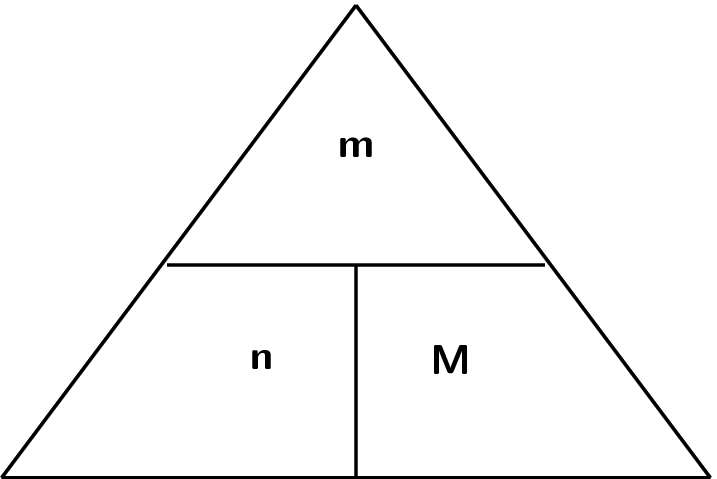
\includegraphics[width=5cm]{col11305.imgs/m38717_CG11C6_001.png} % m38717;CG11C6\_001.png;;;6.0;8.5;
        
      \vspace{2pt}
    \vspace{.1in}
    
    \end{center}

 \end{figure}   

    \addtocounter{footnote}{-0}
    
      \par 
\label{m38717*secfhsst!!!underscore!!!id409}\vspace{.5cm} 
      
      \noindent
      \hspace*{-30pt}
\includegraphics[width=0.5in]{col11305.imgs/pspencil2.png}   \raisebox{25mm}{   
      \begin{mdframed}[linewidth=4, leftmargin=40, rightmargin=40]  
      \begin{exercise}
    \noindent\textbf{Exercise 18.3:  Calculating moles from mass }
      \label{m38717*probfhsst!!!underscore!!!id410}
      \label{m38717*id277635}Calculate the number of moles of copper there are in a sample that weighs \begin{math}127\phantom{\rule{2pt}{0ex}}\mathrm{g}\end{math}.\par 
      
      \vspace{5pt}
      \label{m38717*solfhsst!!!underscore!!!id414}\noindent\textbf{Solution to Exercise } \label{m38717*listfhsst!!!underscore!!!id414}\begin{enumerate}[noitemsep, label=\textbf{Step} \textbf{\arabic*}. ] 
            \leftskip=20pt\rightskip=\leftskip\item  
      \label{m38717*id277680}\nopagebreak\noindent{}
        \settowidth{\mymathboxwidth}{\begin{equation}
    n=\frac{m}{M}\tag{18.6}
      \end{equation}
    }
    \typeout{Columnwidth = \the\columnwidth}\typeout{math as usual width = \the\mymathboxwidth}
    \ifthenelse{\lengthtest{\mymathboxwidth < \columnwidth}}{% if the math fits, do it again, for real
    \begin{equation}
    n=\frac{m}{M}\tag{18.6}
      \end{equation}
    }{% else, if it doesn't fit
    \setlength{\mymathboxwidth}{\columnwidth}
      \addtolength{\mymathboxwidth}{-48pt}
    \par\vspace{12pt}\noindent\begin{minipage}{\columnwidth}
    \parbox[t]{\mymathboxwidth}{\large\begin{math}
    n=\frac{m}{M}\end{math}}\hfill
    \parbox[t]{48pt}{\raggedleft 
    (18.6)}
    \end{minipage}\vspace{12pt}\par
    }% end of conditional for this bit of math
    \typeout{math as usual width = \the\mymathboxwidth}
    
      
      \item  
      \label{m38717*id277705}\nopagebreak\noindent{}
        \settowidth{\mymathboxwidth}{\begin{equation}
    n=\frac{127}{63,55}=2\tag{18.7}
      \end{equation}
    }
    \typeout{Columnwidth = \the\columnwidth}\typeout{math as usual width = \the\mymathboxwidth}
    \ifthenelse{\lengthtest{\mymathboxwidth < \columnwidth}}{% if the math fits, do it again, for real
    \begin{equation}
    n=\frac{127}{63,55}=2\tag{18.7}
      \end{equation}
    }{% else, if it doesn't fit
    \setlength{\mymathboxwidth}{\columnwidth}
      \addtolength{\mymathboxwidth}{-48pt}
    \par\vspace{12pt}\noindent\begin{minipage}{\columnwidth}
    \parbox[t]{\mymathboxwidth}{\large\begin{math}
    n=\frac{127}{63,55}=2\end{math}}\hfill
    \parbox[t]{48pt}{\raggedleft 
    (18.7)}
    \end{minipage}\vspace{12pt}\par
    }% end of conditional for this bit of math
    \typeout{math as usual width = \the\mymathboxwidth}
    
      
      \label{m38717*id277735}There are 2 moles of copper in the sample.\par 
 \end{enumerate}
         

    \end{exercise}
    \end{mdframed}
    }
    \noindent
  
\label{m38717*secfhsst!!!underscore!!!id451}\vspace{.5cm} 
      
      \noindent
      \hspace*{-30pt}
\includegraphics[width=0.5in]{col11305.imgs/pspencil2.png}   \raisebox{25mm}{   
      \begin{mdframed}[linewidth=4, leftmargin=40, rightmargin=40]  
      \begin{exercise}
    \noindent\textbf{Exercise 18.4: Calculating mass from moles }\label{m38717*probfhsst!!!underscore!!!id452}
      \label{m38717*id277751}You are given a 5 mol sample of sodium. What mass of sodium is in the sample?\par 
      
      \vspace{5pt}
      \label{m38717*solfhsst!!!underscore!!!id456}\noindent\textbf{Solution to Exercise } \label{m38717*listfhsst!!!underscore!!!id456}\begin{enumerate}[noitemsep, label=\textbf{Step} \textbf{\arabic*}. ] 
            \leftskip=20pt\rightskip=\leftskip\item  
      \label{m38717*id277797}\nopagebreak\noindent{}
        \settowidth{\mymathboxwidth}{\begin{equation}
    m=n\ensuremath{\times}M\tag{18.8}
      \end{equation}
    }
    \typeout{Columnwidth = \the\columnwidth}\typeout{math as usual width = \the\mymathboxwidth}
    \ifthenelse{\lengthtest{\mymathboxwidth < \columnwidth}}{% if the math fits, do it again, for real
    \begin{equation}
    m=n\ensuremath{\times}M\tag{18.8}
      \end{equation}
    }{% else, if it doesn't fit
    \setlength{\mymathboxwidth}{\columnwidth}
      \addtolength{\mymathboxwidth}{-48pt}
    \par\vspace{12pt}\noindent\begin{minipage}{\columnwidth}
    \parbox[t]{\mymathboxwidth}{\large\begin{math}
    m=n\ensuremath{\times}M\end{math}}\hfill
    \parbox[t]{48pt}{\raggedleft 
    (18.8)}
    \end{minipage}\vspace{12pt}\par
    }% end of conditional for this bit of math
    \typeout{math as usual width = \the\mymathboxwidth}
    
      
      \item  
      \label{m38717*id277822}M\begin{math}{}_{Na}=22,99\phantom{\rule{2pt}{0ex}}\mathrm{g}\ensuremath{\cdot}\mathrm{mol}{}^{-1}\end{math}\par 
      \label{m38717*id277857}Therefore,\par 
      \label{m38717*id277862}\nopagebreak\noindent{}\settowidth{\mymathboxwidth}{\begin{equation}
    m=5\ensuremath{\times}22,99=114,95\phantom{\rule{2pt}{0ex}}\mathrm{g}\tag{18.9}
      \end{equation}
    }
    \typeout{Columnwidth = \the\columnwidth}\typeout{math as usual width = \the\mymathboxwidth}
    \ifthenelse{\lengthtest{\mymathboxwidth < \columnwidth}}{% if the math fits, do it again, for real
    \begin{equation}
    m=5\ensuremath{\times}22,99=114,95\phantom{\rule{2pt}{0ex}}\mathrm{g}\tag{18.9}
      \end{equation}
    }{% else, if it doesn't fit
    \setlength{\mymathboxwidth}{\columnwidth}
      \addtolength{\mymathboxwidth}{-48pt}
    \par\vspace{12pt}\noindent\begin{minipage}{\columnwidth}
    \parbox[t]{\mymathboxwidth}{\large\begin{math}
    m=5\ensuremath{\times}22,99=114,95\phantom{\rule{2pt}{0ex}}\mathrm{g}\end{math}}\hfill
    \parbox[t]{48pt}{\raggedleft 
    (18.9)}
    \end{minipage}\vspace{12pt}\par
    }% end of conditional for this bit of math
    \typeout{math as usual width = \the\mymathboxwidth}
    
      
      \label{m38717*id277898}The sample of sodium has a mass of  \begin{math}114,95\phantom{\rule{2pt}{0ex}}\mathrm{g}\end{math}.\par 
\end{enumerate}
         

    \end{exercise}
    \end{mdframed}
    }
    \noindent
  
\label{m38717*secfhsst!!!underscore!!!id494}\vspace{.5cm} 
      
      \noindent
      \hspace*{-30pt}
\includegraphics[width=0.5in]{col11305.imgs/pspencil2.png}   \raisebox{25mm}{   
      \begin{mdframed}[linewidth=4, leftmargin=40, rightmargin=40]  
      \begin{exercise}
    \noindent\textbf{Exercise 18.5: Calculating atoms from mass }\label{m38717*probfhsst!!!underscore!!!id495}
      \label{m38717*id277914}Calculate the number of atoms there are in a sample of aluminium that weighs \begin{math}80,94\phantom{\rule{2pt}{0ex}}\mathrm{g}\end{math}.\par 
      
      \vspace{5pt}
      \label{m38717*solfhsst!!!underscore!!!id499}\noindent\textbf{Solution to Exercise } \label{m38717*listfhsst!!!underscore!!!id499}\begin{enumerate}[noitemsep, label=\textbf{Step} \textbf{\arabic*}. ] 
            \leftskip=20pt\rightskip=\leftskip\item  
      \label{m38717*id277959}\nopagebreak\noindent{}
        \settowidth{\mymathboxwidth}{\begin{equation}
    n=\frac{m}{M}=\frac{80,94}{26,98}=3\phantom{\rule{2pt}{0ex}}\mathrm{moles}\tag{18.10}
      \end{equation}
    }
    \typeout{Columnwidth = \the\columnwidth}\typeout{math as usual width = \the\mymathboxwidth}
    \ifthenelse{\lengthtest{\mymathboxwidth < \columnwidth}}{% if the math fits, do it again, for real
    \begin{equation}
    n=\frac{m}{M}=\frac{80,94}{26,98}=3\phantom{\rule{2pt}{0ex}}\mathrm{moles}\tag{18.10}
      \end{equation}
    }{% else, if it doesn't fit
    \setlength{\mymathboxwidth}{\columnwidth}
      \addtolength{\mymathboxwidth}{-48pt}
    \par\vspace{12pt}\noindent\begin{minipage}{\columnwidth}
    \parbox[t]{\mymathboxwidth}{\large\begin{math}
    n=\frac{m}{M}=\frac{80,94}{26,98}=3\phantom{\rule{2pt}{0ex}}\mathrm{moles}\end{math}}\hfill
    \parbox[t]{48pt}{\raggedleft 
    (18.10)}
    \end{minipage}\vspace{12pt}\par
    }% end of conditional for this bit of math
    \typeout{math as usual width = \the\mymathboxwidth}
    
      
      \item  
      \label{m38717*id278019}Number of atoms in 3 mol aluminium \begin{math}=3\ensuremath{\times}6,022\ensuremath{\times}10{}^{23}\end{math}\par 
      \label{m38717*id278053}There are \begin{math}18,069\ensuremath{\times}10{}^{23}\end{math} aluminium atoms in a sample of \begin{math}80,94\phantom{\rule{2pt}{0ex}}\mathrm{g}\end{math}.\par 
 \end{enumerate}
         

    \end{exercise}
    \end{mdframed}
    }
    \noindent
  
\label{m38717*secfhsst!!!underscore!!!id539}
            \subsubsection{  Some simple calculations
      }
            \nopagebreak
            
      \label{m38717*id278090}\begin{enumerate}[noitemsep, label=\textbf{\arabic*}. ] 
            \label{m38717*uid24}\item Calculate the number of moles in each of the following samples:
\label{m38717*id278106}\begin{enumerate}[noitemsep, label=\textbf{\alph*}. ] 
            \label{m38717*uid25}\item \begin{math}5,6\phantom{\rule{2pt}{0ex}}\mathrm{g}\end{math} of calcium
\label{m38717*uid26}\item \begin{math}0,02\phantom{\rule{2pt}{0ex}}\mathrm{g}\end{math} of manganese
\label{m38717*uid27}\item \begin{math}40\phantom{\rule{2pt}{0ex}}\mathrm{g}\end{math} of aluminium
\end{enumerate}
                \label{m38717*uid28}\item A lead sinker has a mass of \begin{math}5\phantom{\rule{2pt}{0ex}}\mathrm{g}\end{math}.
\label{m38717*id278159}\begin{enumerate}[noitemsep, label=\textbf{\alph*}. ] 
            \label{m38717*uid29}\item Calculate the number of moles of lead the sinker contains.
\label{m38717*uid30}\item How many lead atoms are in the sinker?
\end{enumerate}
                \label{m38717*uid31}\item Calculate the mass of each of the following samples:
\label{m38717*id278201}\begin{enumerate}[noitemsep, label=\textbf{\alph*}. ] 
            \label{m38717*uid32}\item \begin{math}2,5\phantom{\rule{2pt}{0ex}}\mathrm{mol}\end{math} magnesium
\label{m38717*uid33}\item \begin{math}12\phantom{\rule{2pt}{0ex}}\mathrm{mol}\end{math} lithium
\label{m38717*uid34}\item \begin{math}4,5\ensuremath{\times} 10{}^{25}\end{math} atoms of silicon
\end{enumerate}
                \end{enumerate}
        
      

    
    \label{m38717*cid5}
\par \raisebox{-5 pt}{
\includegraphics[width=0.5cm]{col11305.imgs/summary_www.png}} Find the answers with the shortcodes:
 \par \begin{tabular}[h]{cccccc}
 (1.) lgc  &  (2.) lga  &  (3.) lgx  & \end{tabular}



            \subsection{ Molecules and compounds}
            \nopagebreak
            
      
      \label{m38717*id278284}So far, we have only discussed moles, mass and molar mass in relation to \textsl{elements}. But what happens if we are dealing with a molecule or some other chemical compound? Do the same concepts and rules apply? The answer is 'yes'. However, you need to remember that all your calculations will apply to the \textsl{whole molecule}. So, when you calculate the molar mass of a molecule, you will need to add the molar mass of each atom in that compound. Also, the number of moles will also apply to the whole molecule. For example, if you have one mole of nitric acid (\begin{math}\mathrm{HNO}{}_{3}\end{math}), it means you have \begin{math}6,022\ensuremath{\times}{10}^{23}\end{math} \textbf{molecules} of nitric acid in the sample. This also means that there are \begin{math}6,022\ensuremath{\times}{10}^{23}\end{math} \textbf{atoms} of hydrogen, \begin{math}6,022\ensuremath{\times}{10}^{23}\end{math} \textbf{atoms} of nitrogen and (\begin{math}3\ensuremath{\times}6,022\ensuremath{\times}{10}^{23}\end{math}) \textbf{atoms} of oxygen in the sample.\par 
      \label{m38717*id278429}In a balanced chemical equation, the number that is written in front of the element or compound, shows the \textbf{mole ratio} in which the reactants combine to form a product. If there are no numbers in front of the element symbol, this means the number is '1'.\par 
      \label{m38717*id278442}e.g. \begin{math}{\mathrm{N}}_{2}+3{\mathrm{H}}_{2}\to 2\mathrm{N}{\mathrm{H}}_{3}\end{math}\par 
      \label{m38717*id278488}In this reaction, 1 mole of nitrogen reacts with 3 moles of hydrogen to produce 2 moles of ammonia.\par 
\label{m38717*secfhsst!!!underscore!!!id566}\vspace{.5cm} 
      
      \noindent
      \hspace*{-30pt}
\includegraphics[width=0.5in]{col11305.imgs/pspencil2.png}   \raisebox{25mm}{   
      \begin{mdframed}[linewidth=4, leftmargin=40, rightmargin=40]  
      \begin{exercise}
    \noindent\textbf{Exercise 18.6:  Calculating molar mass }
      \label{m38717*probfhsst!!!underscore!!!id567}
      \label{m38717*id278505}Calculate the molar mass of \begin{math}\mathrm{H}{}_{2}\mathrm{SO}{}_{4}\end{math}.\par 
      
      \vspace{5pt}
      \label{m38717*solfhsst!!!underscore!!!id571}\noindent\textbf{Solution to Exercise } \label{m38717*listfhsst!!!underscore!!!id571}\begin{enumerate}[noitemsep, label=\textbf{Step} \textbf{\arabic*}. ] 
            \leftskip=20pt\rightskip=\leftskip\item  
      \label{m38717*id278575}Hydrogen \begin{math}=1,008\phantom{\rule{2pt}{0ex}}\mathrm{g}\ensuremath{\cdot}\mathrm{mol}{}^{-1}\end{math}; Sulphur = \begin{math}=32,07\phantom{\rule{2pt}{0ex}}\mathrm{g}\ensuremath{\cdot}\mathrm{mol}{}^{-1}\end{math}; Oxygen \begin{math}=16\phantom{\rule{2pt}{0ex}}\mathrm{g}\ensuremath{\cdot}\mathrm{mol}{}^{-1}\end{math}\par 
      \item  
      \label{m38717*id278632}\nopagebreak\noindent{}\settowidth{\mymathboxwidth}{\begin{equation}
    {M}_{\left({H}_{2}S{O}_{4}\right)}=\left(2\ensuremath{\times}1,008\right)+\left(32,07\right)+\left(4\ensuremath{\times}16\right)=98,09\phantom{\rule{2pt}{0ex}}\mathrm{g}\ensuremath{\cdot}{\mathrm{mol}}^{-1}\tag{18.11}
      \end{equation}
    }
    \typeout{Columnwidth = \the\columnwidth}\typeout{math as usual width = \the\mymathboxwidth}
    \ifthenelse{\lengthtest{\mymathboxwidth < \columnwidth}}{% if the math fits, do it again, for real
    \begin{equation}
    {M}_{\left({H}_{2}S{O}_{4}\right)}=\left(2\ensuremath{\times}1,008\right)+\left(32,07\right)+\left(4\ensuremath{\times}16\right)=98,09\phantom{\rule{2pt}{0ex}}\mathrm{g}\ensuremath{\cdot}{\mathrm{mol}}^{-1}\tag{18.11}
      \end{equation}
    }{% else, if it doesn't fit
    \setlength{\mymathboxwidth}{\columnwidth}
      \addtolength{\mymathboxwidth}{-48pt}
    \par\vspace{12pt}\noindent\begin{minipage}{\columnwidth}
    \parbox[t]{\mymathboxwidth}{\large\begin{math}
    {M}_{\left({H}_{2}S{O}_{4}\right)}=\left(2\ensuremath{\times}1,008\right)+\left(32,07\right)+\left(4\ensuremath{\times}16\right)=98,09\phantom{\rule{2pt}{0ex}}\mathrm{g}\ensuremath{\cdot}{\mathrm{mol}}^{-1}\end{math}}\hfill
    \parbox[t]{48pt}{\raggedleft 
    (18.11)}
    \end{minipage}\vspace{12pt}\par
    }% end of conditional for this bit of math
    \typeout{math as usual width = \the\mymathboxwidth}
    
      
\end{enumerate}
         

    \end{exercise}
    \end{mdframed}
    }
    \noindent
  \vspace{-.3cm}
\par
            \label{m38717*secfhsst!!!underscore!!!id641}\vspace{.5cm} 
      
      \noindent
      \hspace*{-30pt}
\includegraphics[width=0.5in]{col11305.imgs/pspencil2.png}   \raisebox{25mm}{   
      \begin{mdframed}[linewidth=4, leftmargin=40, rightmargin=40]  
      \begin{exercise}
    \noindent\textbf{Exercise 18.7:  Calculating moles from mass }
      \label{m38717*probfhsst!!!underscore!!!id642}
      \label{m38717*id278755}Calculate the number of moles there are in \begin{math}1\phantom{\rule{2pt}{0ex}}\mathrm{kg}\end{math} of \begin{math}\mathrm{MgCl}{}_{2}\end{math}.\par 
      
      \vspace{5pt}
      \label{m38717*solfhsst!!!underscore!!!id646}\noindent\textbf{Solution to Exercise } \label{m38717*listfhsst!!!underscore!!!id646}\begin{enumerate}[noitemsep, label=\textbf{Step} \textbf{\arabic*}. ] 
            \leftskip=20pt\rightskip=\leftskip\item  
      \label{m38717*id278813}\nopagebreak\noindent{}
        \settowidth{\mymathboxwidth}{\begin{equation}
    n=\frac{m}{M}\tag{18.12}
      \end{equation}
    }
    \typeout{Columnwidth = \the\columnwidth}\typeout{math as usual width = \the\mymathboxwidth}
    \ifthenelse{\lengthtest{\mymathboxwidth < \columnwidth}}{% if the math fits, do it again, for real
    \begin{equation}
    n=\frac{m}{M}\tag{18.12}
      \end{equation}
    }{% else, if it doesn't fit
    \setlength{\mymathboxwidth}{\columnwidth}
      \addtolength{\mymathboxwidth}{-48pt}
    \par\vspace{12pt}\noindent\begin{minipage}{\columnwidth}
    \parbox[t]{\mymathboxwidth}{\large\begin{math}
    n=\frac{m}{M}\end{math}}\hfill
    \parbox[t]{48pt}{\raggedleft 
    (18.12)}
    \end{minipage}\vspace{12pt}\par
    }% end of conditional for this bit of math
    \typeout{math as usual width = \the\mymathboxwidth}
    
      
      \item  
      \label{m38717*id278839}\begin{enumerate}[noitemsep, label=\textbf{\alph*}. ] 
            \leftskip=20pt\rightskip=\leftskip\label{m38717*uid35}\item Convert mass into grams
\label{m38717*id278854}\nopagebreak\noindent{}\settowidth{\mymathboxwidth}{\begin{equation}
    m=1\mathrm{kg}\ensuremath{\times}1 000=1 000\phantom{\rule{2pt}{0ex}}\mathrm{g}\tag{18.13}
      \end{equation}
    }
    \typeout{Columnwidth = \the\columnwidth}\typeout{math as usual width = \the\mymathboxwidth}
    \ifthenelse{\lengthtest{\mymathboxwidth < \columnwidth}}{% if the math fits, do it again, for real
    \begin{equation}
    m=1\mathrm{kg}\ensuremath{\times}1 000=1 000\phantom{\rule{2pt}{0ex}}\mathrm{g}\tag{18.13}
      \end{equation}
    }{% else, if it doesn't fit
    \setlength{\mymathboxwidth}{\columnwidth}
      \addtolength{\mymathboxwidth}{-48pt}
    \par\vspace{12pt}\noindent\begin{minipage}{\columnwidth}
    \parbox[t]{\mymathboxwidth}{\large\begin{math}
    m=1\mathrm{kg}\ensuremath{\times}1 000=1 000\phantom{\rule{2pt}{0ex}}\mathrm{g}\end{math}}\hfill
    \parbox[t]{48pt}{\raggedleft 
    (18.13)}
    \end{minipage}\vspace{12pt}\par
    }% end of conditional for this bit of math
    \typeout{math as usual width = \the\mymathboxwidth}
    \label{m38717*uid36}\item Calculate the molar mass of \begin{math}\mathrm{MgCl}{}_{2}\end{math}.
\label{m38717*id278912}\nopagebreak\noindent{}\settowidth{\mymathboxwidth}{\begin{equation}
    {M}_{\left({\mathrm{MgCl}}_{2}\right)}=24,31+\left(2\ensuremath{\times}35,45\right)=95,21\phantom{\rule{2pt}{0ex}}\mathrm{g}\ensuremath{\cdot}{\mathrm{mol}}^{-1}\tag{18.14}
      \end{equation}
    }
    \typeout{Columnwidth = \the\columnwidth}\typeout{math as usual width = \the\mymathboxwidth}
    \ifthenelse{\lengthtest{\mymathboxwidth < \columnwidth}}{% if the math fits, do it again, for real
    \begin{equation}
    {M}_{\left({\mathrm{MgCl}}_{2}\right)}=24,31+\left(2\ensuremath{\times}35,45\right)=95,21\phantom{\rule{2pt}{0ex}}\mathrm{g}\ensuremath{\cdot}{\mathrm{mol}}^{-1}\tag{18.14}
      \end{equation}
    }{% else, if it doesn't fit
    \setlength{\mymathboxwidth}{\columnwidth}
      \addtolength{\mymathboxwidth}{-48pt}
    \par\vspace{12pt}\noindent\begin{minipage}{\columnwidth}
    \parbox[t]{\mymathboxwidth}{\large\begin{math}
    {M}_{\left({\mathrm{MgCl}}_{2}\right)}=24,31+\left(2\ensuremath{\times}35,45\right)=95,21\phantom{\rule{2pt}{0ex}}\mathrm{g}\ensuremath{\cdot}{\mathrm{mol}}^{-1}\end{math}}\hfill
    \parbox[t]{48pt}{\raggedleft 
    (18.14)}
    \end{minipage}\vspace{12pt}\par
    }% end of conditional for this bit of math
    \typeout{math as usual width = \the\mymathboxwidth}
    \end{enumerate}
  \pagebreak      
      \item  
      \label{m38717*id279005}\nopagebreak\noindent{}\settowidth{\mymathboxwidth}{\begin{equation}
    n=\frac{1000}{95,21}=10,5\phantom{\rule{2pt}{0ex}}\mathrm{mol}\tag{18.15}
      \end{equation}
    }
    \typeout{Columnwidth = \the\columnwidth}\typeout{math as usual width = \the\mymathboxwidth}
    \ifthenelse{\lengthtest{\mymathboxwidth < \columnwidth}}{% if the math fits, do it again, for real
    \begin{equation}
    n=\frac{1000}{95,21}=10,5\phantom{\rule{2pt}{0ex}}\mathrm{mol}\tag{18.15}
      \end{equation}
    }{% else, if it doesn't fit
    \setlength{\mymathboxwidth}{\columnwidth}
      \addtolength{\mymathboxwidth}{-48pt}
    \par\vspace{12pt}\noindent\begin{minipage}{\columnwidth}
    \parbox[t]{\mymathboxwidth}{\large\begin{math}
    n=\frac{1000}{95,21}=10,5\phantom{\rule{2pt}{0ex}}\mathrm{mol}\end{math}}\hfill
    \parbox[t]{48pt}{\raggedleft 
    (18.15)}
    \end{minipage}\vspace{12pt}\par
    }% end of conditional for this bit of math
    \typeout{math as usual width = \the\mymathboxwidth}
    
      
      \label{m38717*id279046}There are \begin{math}10,5\phantom{\rule{2pt}{0ex}}\mathrm{moles}\end{math} of magnesium chloride in a \begin{math}1\phantom{\rule{2pt}{0ex}}\mathrm{kg}\end{math} sample.\par 
\end{enumerate}
         

    \end{exercise}
    \end{mdframed}
    }
    \noindent
  
\label{m38717*secfhsst!!!underscore!!!id695}\vspace{.5cm} 
      
      \noindent
      \hspace*{-30pt}
\includegraphics[width=0.5in]{col11305.imgs/pspencil2.png}   \raisebox{25mm}{   
      \begin{mdframed}[linewidth=4, leftmargin=40, rightmargin=40]  
      \begin{exercise}
    \noindent\textbf{Exercise 18.8: Calculating the mass of reactants and products }\label{m38717*probfhsst!!!underscore!!!id696}
      \label{m38717*id279063}Barium chloride and sulphuric acid react according to the following equation to produce barium sulphate and hydrochloric acid.\par 
      \label{m38717*id279070}
        \begin{math}{\mathrm{BaCl}}_{2}+{\mathrm{H}}_{2}{\mathrm{SO}}_{4}\to {\mathrm{BaSO}}_{4}+2\mathrm{HCl}\end{math}
      \par 
      \label{m38717*id279141}If you have \begin{math}2\phantom{\rule{2pt}{0ex}}\mathrm{g}\end{math} of \begin{math}\mathrm{BaCl}{}_{2}\end{math}...\par 
      \label{m38717*id279158}\begin{enumerate}[noitemsep, label=\textbf{\arabic*}. ] 
            \leftskip=20pt\rightskip=\leftskip\label{m38717*uid37}\item What quantity (in g) of \begin{math}\mathrm{H}{}_{2}\mathrm{SO}{}_{4}\end{math} will you need for the reaction so that all the barium chloride is used up?
\label{m38717*uid38}\item What mass of \begin{math}\mathrm{HCl}\end{math} is produced during the reaction?
\end{enumerate}
        
      
      \vspace{5pt}
      \label{m38717*solfhsst!!!underscore!!!id743}\noindent\textbf{Solution to Exercise } \label{m38717*listfhsst!!!underscore!!!id743}\begin{enumerate}[noitemsep, label=\textbf{Step} \textbf{\arabic*}. ] 
            \leftskip=20pt\rightskip=\leftskip\item  
      \label{m38717*id279248}\nopagebreak\noindent{}
        \settowidth{\mymathboxwidth}{\begin{equation}
    n=\frac{m}{M}=\frac{2}{208,24}=0,0096\phantom{\rule{2pt}{0ex}}\mathrm{mol}\tag{18.16}
      \end{equation}
    }
    \typeout{Columnwidth = \the\columnwidth}\typeout{math as usual width = \the\mymathboxwidth}
    \ifthenelse{\lengthtest{\mymathboxwidth < \columnwidth}}{% if the math fits, do it again, for real
    \begin{equation}
    n=\frac{m}{M}=\frac{2}{208,24}=0,0096\phantom{\rule{2pt}{0ex}}\mathrm{mol}\tag{18.16}
      \end{equation}
    }{% else, if it doesn't fit
    \setlength{\mymathboxwidth}{\columnwidth}
      \addtolength{\mymathboxwidth}{-48pt}
    \par\vspace{12pt}\noindent\begin{minipage}{\columnwidth}
    \parbox[t]{\mymathboxwidth}{\large\begin{math}
    n=\frac{m}{M}=\frac{2}{208,24}=0,0096\phantom{\rule{2pt}{0ex}}\mathrm{mol}\end{math}}\hfill
    \parbox[t]{48pt}{\raggedleft 
    (18.16)}
    \end{minipage}\vspace{12pt}\par
    }% end of conditional for this bit of math
    \typeout{math as usual width = \the\mymathboxwidth}
    
      
      
      \item  
      \label{m38717*id279344}According to the balanced equation, 1 mole of \begin{math}\mathrm{BaCl}{}_{2}\end{math} will react with 1 mole of \begin{math}\mathrm{H}{}_{2}\mathrm{SO}{}_{4}\end{math}. Therefore, if \begin{math}0,0096\phantom{\rule{2pt}{0ex}}\mathrm{mol}\end{math} of \begin{math}\mathrm{BaCl}{}_{2}\end{math} react, then there must be the same number of moles of \begin{math}\mathrm{H}{}_{2}\mathrm{SO}{}_{4}\end{math} that react because their mole ratio is 1:1.\par 
      \item  
      \label{m38717*id279456}\nopagebreak\noindent{}
        \settowidth{\mymathboxwidth}{\begin{equation}
    m=n\ensuremath{\times}M=0,0096\ensuremath{\times}98,086=0,94\phantom{\rule{2pt}{0ex}}\mathrm{g}\tag{18.17}
      \end{equation}
    }
    \typeout{Columnwidth = \the\columnwidth}\typeout{math as usual width = \the\mymathboxwidth}
    \ifthenelse{\lengthtest{\mymathboxwidth < \columnwidth}}{% if the math fits, do it again, for real
    \begin{equation}
    m=n\ensuremath{\times}M=0,0096\ensuremath{\times}98,086=0,94\phantom{\rule{2pt}{0ex}}\mathrm{g}\tag{18.17}
      \end{equation}
    }{% else, if it doesn't fit
    \setlength{\mymathboxwidth}{\columnwidth}
      \addtolength{\mymathboxwidth}{-48pt}
    \par\vspace{12pt}\noindent\begin{minipage}{\columnwidth}
    \parbox[t]{\mymathboxwidth}{\large\begin{math}
    m=n\ensuremath{\times}M=0,0096\ensuremath{\times}98,086=0,94\phantom{\rule{2pt}{0ex}}\mathrm{g}\end{math}}\hfill
    \parbox[t]{48pt}{\raggedleft 
    (18.17)}
    \end{minipage}\vspace{12pt}\par
    }% end of conditional for this bit of math
    \typeout{math as usual width = \the\mymathboxwidth}
    
      
      \label{m38717*id279505}(answer to 1)\par 
      \item  
      \label{m38717*id279513}According to the balanced equation, 2 moles of \begin{math}\mathrm{HCl}\end{math} are produced for every 1 mole of the two reactants. Therefore the number of moles of \begin{math}\mathrm{HCl}\end{math} produced is (\begin{math}2\ensuremath{\times}0,0096\end{math}), which equals \begin{math}0,0096\phantom{\rule{2pt}{0ex}}\mathrm{moles}\end{math}.\par 
      \item  
      \label{m38717*id279531}\nopagebreak\noindent{}
        \settowidth{\mymathboxwidth}{\begin{equation}
    m=n\ensuremath{\times}M=0,0192\ensuremath{\times}35,73=0,69\phantom{\rule{2pt}{0ex}}\mathrm{g}\tag{18.18}
      \end{equation}
    }
    \typeout{Columnwidth = \the\columnwidth}\typeout{math as usual width = \the\mymathboxwidth}
    \ifthenelse{\lengthtest{\mymathboxwidth < \columnwidth}}{% if the math fits, do it again, for real
    \begin{equation}
    m=n\ensuremath{\times}M=0,0192\ensuremath{\times}35,73=0,69\phantom{\rule{2pt}{0ex}}\mathrm{g}\tag{18.18}
      \end{equation}
    }{% else, if it doesn't fit
    \setlength{\mymathboxwidth}{\columnwidth}
      \addtolength{\mymathboxwidth}{-48pt}
    \par\vspace{12pt}\noindent\begin{minipage}{\columnwidth}
    \parbox[t]{\mymathboxwidth}{\large\begin{math}
    m=n\ensuremath{\times}M=0,0192\ensuremath{\times}35,73=0,69\phantom{\rule{2pt}{0ex}}\mathrm{g}\end{math}}\hfill
    \parbox[t]{48pt}{\raggedleft 
    (18.18)}
    \end{minipage}\vspace{12pt}\par
    }% end of conditional for this bit of math
    \typeout{math as usual width = \the\mymathboxwidth}
    
      
      \label{m38717*id279580}(answer to 2)\par 
\end{enumerate}
         

    \end{exercise}
    \end{mdframed}
    }
    \noindent
  
\label{m38717*secfhsst!!!underscore!!!id832}
            \subsubsection{  Group work : Understanding moles, molecules and Avogadro's number
      }
            \nopagebreak
            
      \label{m38717*id279596}Divide into groups of three and spend about 20 minutes answering the following questions together:\par 
      \label{m38717*id279603}\begin{enumerate}[noitemsep, label=\textbf{\arabic*}. ] 
            \label{m38717*uid39}\item What are the units of the mole? Hint: Check the definition of the mole.
\label{m38717*uid40}\item You have a \begin{math}56\phantom{\rule{2pt}{0ex}}\mathrm{g}\end{math} sample of iron sulphide (\begin{math}\mathrm{FeS}\end{math})
\label{m38717*id279631}\begin{enumerate}[noitemsep, label=\textbf{\alph*}. ] 
            \label{m38717*uid41}\item How many \textbf{moles} of \begin{math}\mathrm{FeS}\end{math} are there in the sample?
\label{m38717*uid42}\item How many \textbf{molecules} of \begin{math}\mathrm{FeS}\end{math} are there in the sample?
\label{m38717*uid43}\item What is the difference between a mole and a molecule?
\end{enumerate}
        \label{m38717*uid44}\item The exact size of \textbf{Avogadro's number} is sometimes difficult to imagine.
\label{m38717*id279703}\begin{enumerate}[noitemsep, label=\textbf{\alph*}. ] 
            \label{m38717*uid45}\item Write down Avogadro's number without using scientific notation.
\label{m38717*uid46}\item How long would it take to count to Avogadro's number? You can assume that you can count two numbers in each second.
\end{enumerate}
        \end{enumerate}
        
      

\label{m38717*eip-945}
    \setcounter{subfigure}{0}


	\begin{figure}[H] % horizontal\label{m38717*moles-1}
    
    
    \textnormal{Khan academy video on the mole - 1}\vspace{.1in} \nopagebreak
  \label{m38717*yt-media2}\label{m38717*yt-video2}
            \raisebox{-5 pt}{ 
\includegraphics[width=0.5cm]{col11305.imgs/summary_www.png}} { (Video:  P10085 )}
      
      \vspace{2pt}
    \vspace{.1in}
    
    

 \end{figure}   

    \addtocounter{footnote}{-0}
    \par \label{m38717*secfhsst!!!underscore!!!id850}
            \subsubsection{  More advanced calculations
      }
            \nopagebreak
            
      \label{m38717*id279756}\begin{enumerate}[noitemsep, label=\textbf{\arabic*}. ] 
            \label{m38717*uid47}\item Calculate the molar mass of the following chemical compounds:
\label{m38717*id279772}\begin{enumerate}[noitemsep, label=\textbf{\alph*}. ] 
            \label{m38717*uid48}\item \begin{math}\mathrm{KOH}\end{math}
\label{m38717*uid49}\item \begin{math}\mathrm{FeCl}{}_{3}\end{math}\label{m38717*uid50}\item \begin{math}{\mathrm{Mg\left(OH\right)}}_{2}\end{math}\end{enumerate}
                \label{m38717*uid51}\item How many moles are present in:
\label{m38717*id279848}\begin{enumerate}[noitemsep, label=\textbf{\alph*}. ] 
            \label{m38717*uid52}\item \begin{math}10\phantom{\rule{2pt}{0ex}}\mathrm{g}\end{math} of \begin{math}Na{}_{2}\end{math}SO\begin{math}{}_{4}\end{math}\label{m38717*uid53}\item \begin{math}34\phantom{\rule{2pt}{0ex}}\mathrm{g}\end{math} of \begin{math}\mathrm{Ca\left(OH\right)}{}_{2}\end{math}\label{m38717*uid54}\item \begin{math}2,45\ensuremath{\times}10{}^{23}\end{math} molecules of \begin{math}\mathrm{CH}{}_{4}\end{math}?
\end{enumerate}
                \label{m38717*uid55}\item For a sample of \begin{math}0,2\phantom{\rule{2pt}{0ex}}\mathrm{moles}\end{math} of potassium bromide (\begin{math}\mathrm{KBr}\end{math}), calculate...
\label{m38717*id279964}\begin{enumerate}[noitemsep, label=\textbf{\alph*}. ] 
            \label{m38717*uid56}\item the number of moles of \begin{math}{\mathrm{K}}^{+}\end{math} ions
\label{m38717*uid57}\item the number of moles of \begin{math}{\mathrm{Br}}^{-}\end{math} ions
\end{enumerate}
                \label{m38717*uid58}\item You have a sample containing \begin{math}3\phantom{\rule{2pt}{0ex}}\mathrm{moles}\end{math} of calcium chloride.
\label{m38717*id280031}\begin{enumerate}[noitemsep, label=\textbf{\alph*}. ] 
            \label{m38717*uid59}\item What is the chemical formula of calcium chloride?
\label{m38717*uid60}\item How many calcium atoms are in the sample?
\end{enumerate}
                \label{m38717*uid61}\item Calculate the mass of:
\label{m38717*id280072}\begin{enumerate}[noitemsep, label=\textbf{\alph*}. ] 
            \label{m38717*uid62}\item \begin{math}3\phantom{\rule{2pt}{0ex}}\mathrm{moles}\end{math} of \begin{math}\mathrm{NH}{}_{4}\mathrm{OH}\end{math}
\label{m38717*uid63}\item \begin{math}4,2\phantom{\rule{2pt}{0ex}}\mathrm{moles}\end{math} of \begin{math}Ca\left(\mathrm{NO}{}_{3}\right){}_{2}\end{math}\end{enumerate}
                \label{m38717*uid64}\item \begin{math}96,2\phantom{\rule{2pt}{0ex}}\mathrm{g}\end{math} sulphur reacts with an unknown quantity of zinc according to the following equation:
\begin{math}Zn+\mathrm{S}\to \mathrm{ZnS}\end{math}\label{m38717*id280179}\begin{enumerate}[noitemsep, label=\textbf{\alph*}. ] 
            \label{m38717*uid65}\item What mass of zinc will you need for the reaction, if all the sulphur is to be used up?
\label{m38717*uid66}\item What mass of zinc sulphide will this reaction produce?
\end{enumerate}
                \label{m38717*uid67}\item Calcium chloride reacts with carbonic acid to produce calcium carbonate and hydrochloric acid according to the following equation:
\begin{math}{\mathrm{CaCl}}_{2}+{\mathrm{H}}_{2}{\mathrm{CO}}_{3}\to {\mathrm{CaCO}}_{3}+2\mathrm{HCl}\end{math}
If you want to produce \begin{math}10\phantom{\rule{2pt}{0ex}}\mathrm{g}\end{math} of calcium carbonate through this chemical reaction, what quantity (in g) of calcium chloride will you need at the start of the reaction?\newline
            
\end{enumerate}
        
      

    
  
    
  \label{m38717**end}
          
\par \raisebox{-5 pt}{
\includegraphics[width=0.5cm]{col11305.imgs/summary_www.png}} Find the answers with the shortcodes:
 \par \begin{tabular}[h]{cccccc}
 (1.) lgC  &  (2.) lgr  &  (3.) lg1  &  (4.) lgY  &  (5.) lgg  &  (6.) lg4  &  (7.) lg2  & \end{tabular}



         \section{ Stoichiometry and composition}
    \nopagebreak
            \label{m38712} $ \hspace{-5pt}\begin{array}{cccccccccccc}   
\includegraphics[width=0.75cm]{col11305.imgs/summary_fullmarks.png} &   
\includegraphics[width=0.75cm]{col11305.imgs/summary_video.png} &   
\includegraphics[width=0.75cm]{col11305.imgs/summary_presentation.png} &   \end{array} $ \hspace{2 pt}\raisebox{-5 pt}{} {(section shortcode: P10086 )} \par 
    
    
    
    
    
    
  
    \label{m38712*cid6}
            \subsection{ The Composition of Substances}
            \nopagebreak
            
      
      \label{m38712*id280317}The \textbf{empirical formula} of a chemical compound is a simple expression of the relative number of each type of atom in that compound. In contrast, the \textbf{molecular formula} of a chemical compound gives the actual number of atoms of each element found in a molecule of that compound.\par 
\label{m38712*fhsst!!!underscore!!!id885}\begin{definition}
	  \begin{tabular*}{15 cm}{m{15 mm}m{}}
	\hspace*{-50pt}  
\includegraphics[width=0.5in]{col11305.imgs/psflag2.png}   & \Definition{   \label{id2501853}\textbf{ Empirical formula }} { \label{m38712*meaningfhsst!!!underscore!!!id885}
      \label{m38712*id280341}The empirical formula of a chemical compound gives the relative number of each type of atom in that compound. \par 
       } 
      \end{tabular*}
      \end{definition}

\label{m38712*fhsst!!!underscore!!!id888}\begin{definition}
	  \begin{tabular*}{15 cm}{m{15 mm}m{}}
	\hspace*{-50pt}  
\includegraphics[width=0.5in]{col11305.imgs/psflag2.png}   & \Definition{   \label{id2501878}\textbf{ Molecular formula }} { \label{m38712*meaningfhsst!!!underscore!!!id888}
      \label{m38712*id280360}The molecular formula of a chemical compound gives the exact number of atoms of each element in one molecule of that compound. \par 
       } 
      \end{tabular*}
      \end{definition}

      \label{m38712*id280372}The compound \textsl{ethanoic acid} for example, has the molecular formula \begin{math}\mathrm{CH}{}_{3}\mathrm{COOH}\end{math} or simply \begin{math}\mathrm{C}{}_{2}\mathrm{H}{}_{4}\mathrm{O}{}_{2}\end{math}. In one molecule of this acid, there are two carbon atoms, four hydrogen atoms and two oxygen atoms. The ratio of atoms in the compound is 2:4:2, which can be simplified to 1:2:1. Therefore, the empirical formula for this compound is \begin{math}\mathrm{CH}{}_{2}\mathrm{O}\end{math}. The empirical formula contains the smallest whole number ratio of the elements that make up a compound.\par 
      \label{m38712*id280450}Knowing either the empirical or molecular formula of a compound, can help to determine its composition in more detail. The opposite is also true. Knowing the \textsl{composition} of a substance can help you to determine its formula. There are four different types of composition problems that you might come across:\par 
      \label{m38712*id280463}\begin{enumerate}[noitemsep, label=\textbf{\arabic*}. ] 
            \label{m38712*uid68}\item Problems where you will be given the formula of the substance and asked to calculate the percentage by mass of each element in the substance.
\label{m38712*uid69}\item Problems where you will be given the percentage composition and asked to calculate the formula.
\label{m38712*uid70}\item Problems where you will be given the products of a chemical reaction and asked to calculate the formula of one of the reactants. These are often referred to as combustion analysis problems.
\label{m38712*uid7021}\item Problems where you will be asked to find number of moles of waters of crystallisation.
\end{enumerate}
        
\par
            \label{m38712*secfhsst!!!underscore!!!id901}\vspace{.5cm} 
      
      \noindent
      \hspace*{-30pt}
\includegraphics[width=0.5in]{col11305.imgs/pspencil2.png}   \raisebox{25mm}{   
      \begin{mdframed}[linewidth=4, leftmargin=40, rightmargin=40]  
      \begin{exercise}
    \noindent\textbf{Exercise 18.9:  Calculating the percentage by mass of elements in a compound }
      \label{m38712*probfhsst!!!underscore!!!id902}
      \label{m38712*id280520}Calculate the percentage that each element contributes to the overall mass of sulphuric acid (\begin{math}{\mathrm{H}}_{2}{\mathrm{SO}}_{4}\end{math}).\par 
      
      \vspace{5pt}
      \label{m38712*solfhsst!!!underscore!!!id906}\noindent\textbf{Solution to Exercise } \label{m38712*listfhsst!!!underscore!!!id906}\begin{enumerate}[noitemsep, label=\textbf{Step} \textbf{\arabic*}. ] 
            \leftskip=20pt\rightskip=\leftskip\item  
      \label{m38712*id280575}\begin{math}\mathrm{Hydrogen}=1,008\ensuremath{\times}2=2,016\phantom{\rule{2pt}{0ex}}\mathrm{u}\end{math}\par 
      \label{m38712*id280588}\begin{math}\mathrm{Sulphur}=32,07\phantom{\rule{2pt}{0ex}}\mathrm{u}\end{math}\par 
      \label{m38712*id280591}\begin{math}\mathrm{Oxygen}=4\ensuremath{\times}16=64\phantom{\rule{2pt}{0ex}}\mathrm{u}\end{math}\par 
      
      \item  
      \label{m38712*id280625}Use the calculations in the previous step to calculate the molecular mass of sulphuric acid.\par 
      \label{m38712*id280629}\nopagebreak\noindent{}
        \settowidth{\mymathboxwidth}{\begin{equation}
    \mathrm{Mass}=2,016+32,07+64=98,09\phantom{\rule{2pt}{0ex}}\mathrm{u}\tag{18.19}
      \end{equation}
    }
    \typeout{Columnwidth = \the\columnwidth}\typeout{math as usual width = \the\mymathboxwidth}
    \ifthenelse{\lengthtest{\mymathboxwidth < \columnwidth}}{% if the math fits, do it again, for real
    \begin{equation}
    \mathrm{Mass}=2,016+32,07+64=98,09\phantom{\rule{2pt}{0ex}}\mathrm{u}\tag{18.19}
      \end{equation}
    }{% else, if it doesn't fit
    \setlength{\mymathboxwidth}{\columnwidth}
      \addtolength{\mymathboxwidth}{-48pt}
    \par\vspace{12pt}\noindent\begin{minipage}{\columnwidth}
    \parbox[t]{\mymathboxwidth}{\large\begin{math}
    \mathrm{Mass}=2,016+32,07+64=98,09\phantom{\rule{2pt}{0ex}}\mathrm{u}\end{math}}\hfill
    \parbox[t]{48pt}{\raggedleft 
    (18.19)}
    \end{minipage}\vspace{12pt}\par
    }% end of conditional for this bit of math
    \typeout{math as usual width = \the\mymathboxwidth}
    
      
      \item  
      \label{m38712*id280685}Use the equation:\par 
      \label{m38712*id280688}\begin{math}\mathrm{Percentage\; by\; mass}=\frac{\mathrm{atomic\; mass}}{\mathrm{molecular\; mass\; of\; H}{}_{2}\mathrm{SO}{}_{4}}\ensuremath{\times}100\%\end{math}\par 
      \label{m38712*id280729}
        \textsl{Hydrogen}
      \par 
      \label{m38712*id280735}\nopagebreak\noindent{}
        \settowidth{\mymathboxwidth}{\begin{equation}
    \frac{2,016}{98,09}\ensuremath{\times}100\%=2,06\%\tag{18.20}
      \end{equation}
    }
    \typeout{Columnwidth = \the\columnwidth}\typeout{math as usual width = \the\mymathboxwidth}
    \ifthenelse{\lengthtest{\mymathboxwidth < \columnwidth}}{% if the math fits, do it again, for real
    \begin{equation}
    \frac{2,016}{98,09}\ensuremath{\times}100\%=2,06\%\tag{18.20}
      \end{equation}
    }{% else, if it doesn't fit
    \setlength{\mymathboxwidth}{\columnwidth}
      \addtolength{\mymathboxwidth}{-48pt}
    \par\vspace{12pt}\noindent\begin{minipage}{\columnwidth}
    \parbox[t]{\mymathboxwidth}{\large\begin{math}
    \frac{2,016}{98,09}\ensuremath{\times}100\%=2,06\%\end{math}}\hfill
    \parbox[t]{48pt}{\raggedleft 
    (18.20)}
    \end{minipage}\vspace{12pt}\par
    }% end of conditional for this bit of math
    \typeout{math as usual width = \the\mymathboxwidth}
    
      
      \label{m38712*id280780}
        \textsl{Sulphur}
      \par 
      \label{m38712*id280786}\nopagebreak\noindent{}
        \settowidth{\mymathboxwidth}{\begin{equation}
    \frac{32,07}{98,09}\ensuremath{\times}100\%=32,69\%\tag{18.21}
      \end{equation}
    }
    \typeout{Columnwidth = \the\columnwidth}\typeout{math as usual width = \the\mymathboxwidth}
    \ifthenelse{\lengthtest{\mymathboxwidth < \columnwidth}}{% if the math fits, do it again, for real
    \begin{equation}
    \frac{32,07}{98,09}\ensuremath{\times}100\%=32,69\%\tag{18.21}
      \end{equation}
    }{% else, if it doesn't fit
    \setlength{\mymathboxwidth}{\columnwidth}
      \addtolength{\mymathboxwidth}{-48pt}
    \par\vspace{12pt}\noindent\begin{minipage}{\columnwidth}
    \parbox[t]{\mymathboxwidth}{\large\begin{math}
    \frac{32,07}{98,09}\ensuremath{\times}100\%=32,69\%\end{math}}\hfill
    \parbox[t]{48pt}{\raggedleft 
    (18.21)}
    \end{minipage}\vspace{12pt}\par
    }% end of conditional for this bit of math
    \typeout{math as usual width = \the\mymathboxwidth}
    
      
      \label{m38712*id280831}
        \textsl{Oxygen}
      \par 
      \label{m38712*id280837}\nopagebreak\noindent{}
        \settowidth{\mymathboxwidth}{\begin{equation}
    \frac{64}{98,09}\ensuremath{\times}100\%=65,25\%\tag{18.22}
      \end{equation}
    }
    \typeout{Columnwidth = \the\columnwidth}\typeout{math as usual width = \the\mymathboxwidth}
    \ifthenelse{\lengthtest{\mymathboxwidth < \columnwidth}}{% if the math fits, do it again, for real
    \begin{equation}
    \frac{64}{98,09}\ensuremath{\times}100\%=65,25\%\tag{18.22}
      \end{equation}
    }{% else, if it doesn't fit
    \setlength{\mymathboxwidth}{\columnwidth}
      \addtolength{\mymathboxwidth}{-48pt}
    \par\vspace{12pt}\noindent\begin{minipage}{\columnwidth}
    \parbox[t]{\mymathboxwidth}{\large\begin{math}
    \frac{64}{98,09}\ensuremath{\times}100\%=65,25\%\end{math}}\hfill
    \parbox[t]{48pt}{\raggedleft 
    (18.22)}
    \end{minipage}\vspace{12pt}\par
    }% end of conditional for this bit of math
    \typeout{math as usual width = \the\mymathboxwidth}
    
      
      \label{m38712*id280876}(You should check at the end that these percentages add up to 100\%!)\par 
      \label{m38712*id280880}In other words, in one molecule of sulphuric acid, hydrogen makes up 2,06\% of the mass of the compound, sulphur makes up 32,69\% and oxygen makes up 65,25\%.\par 
\end{enumerate}
         

    \end{exercise}
    \end{mdframed}
    }
    \noindent
  
\label{m38712*secfhsst!!!underscore!!!id1029}\vspace{.5cm} 
      
      \noindent
      \hspace*{-30pt}
\includegraphics[width=0.5in]{col11305.imgs/pspencil2.png}   \raisebox{25mm}{   
      \begin{mdframed}[linewidth=4, leftmargin=40, rightmargin=40]  
      \begin{exercise}
    \noindent\textbf{Exercise 18.10:  Determining the empirical formula of a compound }
      \label{m38712*probfhsst!!!underscore!!!id1030}
      \label{m38712*id280897}A compound contains 52.2\% carbon (\begin{math}\mathrm{C}\end{math}), 13.0\% hydrogen (\begin{math}\mathrm{H}\end{math}) and 34.8\% oxygen (\begin{math}\mathrm{O}\end{math}). Determine its empirical formula.\par 
      
      \vspace{5pt}
      \label{m38712*solfhsst!!!underscore!!!id1034}\noindent\textbf{Solution to Exercise } \label{m38712*listfhsst!!!underscore!!!id1034}\begin{enumerate}[noitemsep, label=\textbf{Step} \textbf{\arabic*}. ] 
            \leftskip=20pt\rightskip=\leftskip\item  
      \label{m38712*id280928}Carbon \begin{math}=52,2\phantom{\rule{2pt}{0ex}}\mathrm{g}\end{math}, hydrogen \begin{math}=13,0\phantom{\rule{2pt}{0ex}}\mathrm{g}\end{math} and oxygen \begin{math}=34,8\phantom{\rule{2pt}{0ex}}\mathrm{g}\end{math}\par 
      
      \item  
      \label{m38712*id280954}\nopagebreak\noindent{}
        \settowidth{\mymathboxwidth}{\begin{equation}
    n=\frac{m}{M}\tag{18.23}
      \end{equation}
    }
    \typeout{Columnwidth = \the\columnwidth}\typeout{math as usual width = \the\mymathboxwidth}
    \ifthenelse{\lengthtest{\mymathboxwidth < \columnwidth}}{% if the math fits, do it again, for real
    \begin{equation}
    n=\frac{m}{M}\tag{18.23}
      \end{equation}
    }{% else, if it doesn't fit
    \setlength{\mymathboxwidth}{\columnwidth}
      \addtolength{\mymathboxwidth}{-48pt}
    \par\vspace{12pt}\noindent\begin{minipage}{\columnwidth}
    \parbox[t]{\mymathboxwidth}{\large\begin{math}
    n=\frac{m}{M}\end{math}}\hfill
    \parbox[t]{48pt}{\raggedleft 
    (18.23)}
    \end{minipage}\vspace{12pt}\par
    }% end of conditional for this bit of math
    \typeout{math as usual width = \the\mymathboxwidth}
    
      
      \label{m38712*id280975}Therefore,\par 
      \label{m38712*id280978}\nopagebreak\noindent{}
        \settowidth{\mymathboxwidth}{\begin{equation}
    n\left(\mathrm{Carbon}\right)=\frac{52,2}{12,01}=4,35\mathrm{mol}\tag{18.24}
      \end{equation}
    }
    \typeout{Columnwidth = \the\columnwidth}\typeout{math as usual width = \the\mymathboxwidth}
    \ifthenelse{\lengthtest{\mymathboxwidth < \columnwidth}}{% if the math fits, do it again, for real
    \begin{equation}
    n\left(\mathrm{Carbon}\right)=\frac{52,2}{12,01}=4,35\mathrm{mol}\tag{18.24}
      \end{equation}
    }{% else, if it doesn't fit
    \setlength{\mymathboxwidth}{\columnwidth}
      \addtolength{\mymathboxwidth}{-48pt}
    \par\vspace{12pt}\noindent\begin{minipage}{\columnwidth}
    \parbox[t]{\mymathboxwidth}{\large\begin{math}
    n\left(\mathrm{Carbon}\right)=\frac{52,2}{12,01}=4,35\mathrm{mol}\end{math}}\hfill
    \parbox[t]{48pt}{\raggedleft 
    (18.24)}
    \end{minipage}\vspace{12pt}\par
    }% end of conditional for this bit of math
    \typeout{math as usual width = \the\mymathboxwidth}
    
      
      \label{m38712*id281042}\nopagebreak\noindent{}
        \settowidth{\mymathboxwidth}{\begin{equation}
    n\left(\mathrm{Hydrogen}\right)=\frac{13,0}{1,008}=12,90\mathrm{mol}\tag{18.25}
      \end{equation}
    }
    \typeout{Columnwidth = \the\columnwidth}\typeout{math as usual width = \the\mymathboxwidth}
    \ifthenelse{\lengthtest{\mymathboxwidth < \columnwidth}}{% if the math fits, do it again, for real
    \begin{equation}
    n\left(\mathrm{Hydrogen}\right)=\frac{13,0}{1,008}=12,90\mathrm{mol}\tag{18.25}
      \end{equation}
    }{% else, if it doesn't fit
    \setlength{\mymathboxwidth}{\columnwidth}
      \addtolength{\mymathboxwidth}{-48pt}
    \par\vspace{12pt}\noindent\begin{minipage}{\columnwidth}
    \parbox[t]{\mymathboxwidth}{\large\begin{math}
    n\left(\mathrm{Hydrogen}\right)=\frac{13,0}{1,008}=12,90\mathrm{mol}\end{math}}\hfill
    \parbox[t]{48pt}{\raggedleft 
    (18.25)}
    \end{minipage}\vspace{12pt}\par
    }% end of conditional for this bit of math
    \typeout{math as usual width = \the\mymathboxwidth}
    
      
      \label{m38712*id281111}\nopagebreak\noindent{}
        \settowidth{\mymathboxwidth}{\begin{equation}
    n\left(\mathrm{Oxygen}\right)=\frac{34,8}{16}=2,18\mathrm{mol}\tag{18.26}
      \end{equation}
    }
    \typeout{Columnwidth = \the\columnwidth}\typeout{math as usual width = \the\mymathboxwidth}
    \ifthenelse{\lengthtest{\mymathboxwidth < \columnwidth}}{% if the math fits, do it again, for real
    \begin{equation}
    n\left(\mathrm{Oxygen}\right)=\frac{34,8}{16}=2,18\mathrm{mol}\tag{18.26}
      \end{equation}
    }{% else, if it doesn't fit
    \setlength{\mymathboxwidth}{\columnwidth}
      \addtolength{\mymathboxwidth}{-48pt}
    \par\vspace{12pt}\noindent\begin{minipage}{\columnwidth}
    \parbox[t]{\mymathboxwidth}{\large\begin{math}
    n\left(\mathrm{Oxygen}\right)=\frac{34,8}{16}=2,18\mathrm{mol}\end{math}}\hfill
    \parbox[t]{48pt}{\raggedleft 
    (18.26)}
    \end{minipage}\vspace{12pt}\par
    }% end of conditional for this bit of math
    \typeout{math as usual width = \the\mymathboxwidth}
    
      
      \item  
      \label{m38712*id281175}In this case, the smallest number of moles is 2.18. Therefore...\par 
      \label{m38712*id281179}
        \textsl{Carbon}
      \par 
      \label{m38712*id281185}\nopagebreak\noindent{}
        \settowidth{\mymathboxwidth}{\begin{equation}
    \frac{4,35}{2,18}=2\tag{18.27}
      \end{equation}
    }
    \typeout{Columnwidth = \the\columnwidth}\typeout{math as usual width = \the\mymathboxwidth}
    \ifthenelse{\lengthtest{\mymathboxwidth < \columnwidth}}{% if the math fits, do it again, for real
    \begin{equation}
    \frac{4,35}{2,18}=2\tag{18.27}
      \end{equation}
    }{% else, if it doesn't fit
    \setlength{\mymathboxwidth}{\columnwidth}
      \addtolength{\mymathboxwidth}{-48pt}
    \par\vspace{12pt}\noindent\begin{minipage}{\columnwidth}
    \parbox[t]{\mymathboxwidth}{\large\begin{math}
    \frac{4,35}{2,18}=2\end{math}}\hfill
    \parbox[t]{48pt}{\raggedleft 
    (18.27)}
    \end{minipage}\vspace{12pt}\par
    }% end of conditional for this bit of math
    \typeout{math as usual width = \the\mymathboxwidth}
    
      
      \label{m38712*id281217}
        \textsl{Hydrogen}
      \par 
      \label{m38712*id281223}\nopagebreak\noindent{}
        \settowidth{\mymathboxwidth}{\begin{equation}
    \frac{12,90}{2,18}=6\tag{18.28}
      \end{equation}
    }
    \typeout{Columnwidth = \the\columnwidth}\typeout{math as usual width = \the\mymathboxwidth}
    \ifthenelse{\lengthtest{\mymathboxwidth < \columnwidth}}{% if the math fits, do it again, for real
    \begin{equation}
    \frac{12,90}{2,18}=6\tag{18.28}
      \end{equation}
    }{% else, if it doesn't fit
    \setlength{\mymathboxwidth}{\columnwidth}
      \addtolength{\mymathboxwidth}{-48pt}
    \par\vspace{12pt}\noindent\begin{minipage}{\columnwidth}
    \parbox[t]{\mymathboxwidth}{\large\begin{math}
    \frac{12,90}{2,18}=6\end{math}}\hfill
    \parbox[t]{48pt}{\raggedleft 
    (18.28)}
    \end{minipage}\vspace{12pt}\par
    }% end of conditional for this bit of math
    \typeout{math as usual width = \the\mymathboxwidth}
    
      
      \label{m38712*id281254}
        \textsl{Oxygen}
      \par 
      \label{m38712*id281261}\nopagebreak\noindent{}
        \settowidth{\mymathboxwidth}{\begin{equation}
    \frac{2,18}{2,18}=1\tag{18.29}
      \end{equation}
    }
    \typeout{Columnwidth = \the\columnwidth}\typeout{math as usual width = \the\mymathboxwidth}
    \ifthenelse{\lengthtest{\mymathboxwidth < \columnwidth}}{% if the math fits, do it again, for real
    \begin{equation}
    \frac{2,18}{2,18}=1\tag{18.29}
      \end{equation}
    }{% else, if it doesn't fit
    \setlength{\mymathboxwidth}{\columnwidth}
      \addtolength{\mymathboxwidth}{-48pt}
    \par\vspace{12pt}\noindent\begin{minipage}{\columnwidth}
    \parbox[t]{\mymathboxwidth}{\large\begin{math}
    \frac{2,18}{2,18}=1\end{math}}\hfill
    \parbox[t]{48pt}{\raggedleft 
    (18.29)}
    \end{minipage}\vspace{12pt}\par
    }% end of conditional for this bit of math
    \typeout{math as usual width = \the\mymathboxwidth}
    
      
      \label{m38712*id281292}Therefore the empirical formula of this substance is: \begin{math}{\mathrm{C}}_{2}{\mathrm{H}}_{6}\mathrm{O}\end{math}. Do you recognise this compound?\par 
\end{enumerate}
         

    \end{exercise}
    \end{mdframed}
    }
    \noindent
  
\label{m38712*secfhsst!!!underscore!!!id1235}\vspace{.5cm} 
      
      \noindent
      \hspace*{-30pt}
\includegraphics[width=0.5in]{col11305.imgs/pspencil2.png}   \raisebox{25mm}{   
      \begin{mdframed}[linewidth=4, leftmargin=40, rightmargin=40]  
      \begin{exercise}
    \noindent\textbf{Exercise 18.11:  Determining the formula of a compound }
      \label{m38712*probfhsst!!!underscore!!!id1236}
      \label{m38712*id281333}\begin{math}207\phantom{\rule{2pt}{0ex}}\mathrm{g}\end{math} of lead combines with oxygen to form \begin{math}239\phantom{\rule{2pt}{0ex}}\mathrm{g}\end{math} of a lead oxide. Use this information to work out the formula of the lead oxide (Relative atomic masses: \begin{math}Pb=207\phantom{\rule{2pt}{0ex}}\mathrm{u}\end{math} and \begin{math}\mathrm{O}=16\phantom{\rule{2pt}{0ex}}\mathrm{u}\end{math}).\par 
      \pagebreak
      \vspace{5pt}
      \label{m38712*solfhsst!!!underscore!!!id1240}\noindent\textbf{Solution to Exercise } \label{m38712*listfhsst!!!underscore!!!id1240}\begin{enumerate}[noitemsep, label=\textbf{Step} \textbf{\arabic*}. ] 
            \leftskip=20pt\rightskip=\leftskip\item  
      \label{m38712*id281379}\nopagebreak\noindent{}\settowidth{\mymathboxwidth}{\begin{equation}
    239-207=32\phantom{\rule{2pt}{0ex}}\mathrm{g}\tag{18.30}
      \end{equation}
    }
    \typeout{Columnwidth = \the\columnwidth}\typeout{math as usual width = \the\mymathboxwidth}
    \ifthenelse{\lengthtest{\mymathboxwidth < \columnwidth}}{% if the math fits, do it again, for real
    \begin{equation}
    239-207=32\phantom{\rule{2pt}{0ex}}\mathrm{g}\tag{18.30}
      \end{equation}
    }{% else, if it doesn't fit
    \setlength{\mymathboxwidth}{\columnwidth}
      \addtolength{\mymathboxwidth}{-48pt}
    \par\vspace{12pt}\noindent\begin{minipage}{\columnwidth}
    \parbox[t]{\mymathboxwidth}{\large\begin{math}
    239-207=32\phantom{\rule{2pt}{0ex}}\mathrm{g}\end{math}}\hfill
    \parbox[t]{48pt}{\raggedleft 
    (18.30)}
    \end{minipage}\vspace{12pt}\par
    }% end of conditional for this bit of math
    \typeout{math as usual width = \the\mymathboxwidth}
    
      
      \item  
      \label{m38712*id281407}\nopagebreak\noindent{}
        \settowidth{\mymathboxwidth}{\begin{equation}
    n=\frac{m}{M}\tag{18.31}
      \end{equation}
    }
    \typeout{Columnwidth = \the\columnwidth}\typeout{math as usual width = \the\mymathboxwidth}
    \ifthenelse{\lengthtest{\mymathboxwidth < \columnwidth}}{% if the math fits, do it again, for real
    \begin{equation}
    n=\frac{m}{M}\tag{18.31}
      \end{equation}
    }{% else, if it doesn't fit
    \setlength{\mymathboxwidth}{\columnwidth}
      \addtolength{\mymathboxwidth}{-48pt}
    \par\vspace{12pt}\noindent\begin{minipage}{\columnwidth}
    \parbox[t]{\mymathboxwidth}{\large\begin{math}
    n=\frac{m}{M}\end{math}}\hfill
    \parbox[t]{48pt}{\raggedleft 
    (18.31)}
    \end{minipage}\vspace{12pt}\par
    }% end of conditional for this bit of math
    \typeout{math as usual width = \the\mymathboxwidth}
    
      
      \label{m38712*id281427}
        \textsl{Lead}
      \par 
      \label{m38712*id281433}\nopagebreak\noindent{}
        \settowidth{\mymathboxwidth}{\begin{equation}
    \frac{207}{207}=1\phantom{\rule{2pt}{0ex}}\mathrm{mol}\tag{18.32}
      \end{equation}
    }
    \typeout{Columnwidth = \the\columnwidth}\typeout{math as usual width = \the\mymathboxwidth}
    \ifthenelse{\lengthtest{\mymathboxwidth < \columnwidth}}{% if the math fits, do it again, for real
    \begin{equation}
    \frac{207}{207}=1\phantom{\rule{2pt}{0ex}}\mathrm{mol}\tag{18.32}
      \end{equation}
    }{% else, if it doesn't fit
    \setlength{\mymathboxwidth}{\columnwidth}
      \addtolength{\mymathboxwidth}{-48pt}
    \par\vspace{12pt}\noindent\begin{minipage}{\columnwidth}
    \parbox[t]{\mymathboxwidth}{\large\begin{math}
    \frac{207}{207}=1\phantom{\rule{2pt}{0ex}}\mathrm{mol}\end{math}}\hfill
    \parbox[t]{48pt}{\raggedleft 
    (18.32)}
    \end{minipage}\vspace{12pt}\par
    }% end of conditional for this bit of math
    \typeout{math as usual width = \the\mymathboxwidth}
    
      
      \label{m38712*id281460}
        \textsl{Oxygen}
      \par 
      \label{m38712*id281467}\nopagebreak\noindent{}
        \settowidth{\mymathboxwidth}{\begin{equation}
    \frac{32}{16}=2\phantom{\rule{2pt}{0ex}}\mathrm{mol}\tag{18.33}
      \end{equation}
    }
    \typeout{Columnwidth = \the\columnwidth}\typeout{math as usual width = \the\mymathboxwidth}
    \ifthenelse{\lengthtest{\mymathboxwidth < \columnwidth}}{% if the math fits, do it again, for real
    \begin{equation}
    \frac{32}{16}=2\phantom{\rule{2pt}{0ex}}\mathrm{mol}\tag{18.33}
      \end{equation}
    }{% else, if it doesn't fit
    \setlength{\mymathboxwidth}{\columnwidth}
      \addtolength{\mymathboxwidth}{-48pt}
    \par\vspace{12pt}\noindent\begin{minipage}{\columnwidth}
    \parbox[t]{\mymathboxwidth}{\large\begin{math}
    \frac{32}{16}=2\phantom{\rule{2pt}{0ex}}\mathrm{mol}\end{math}}\hfill
    \parbox[t]{48pt}{\raggedleft 
    (18.33)}
    \end{minipage}\vspace{12pt}\par
    }% end of conditional for this bit of math
    \typeout{math as usual width = \the\mymathboxwidth}
    
      
      \item  
      \label{m38712*id281498}The mole ratio of \begin{math}Pb:\mathrm{O}\end{math} in the product is 1:2, which means that for every atom of lead, there will be two atoms of oxygen. The formula of the compound is \begin{math}\mathrm{PbO}{}_{2}\end{math}.\par 
 \end{enumerate}
         

    \end{exercise}
    \end{mdframed}
    }
    \noindent
  
\label{m38712*secfhsst!!!underscore!!!id1308}\vspace{.5cm} 
      
      \noindent
      \hspace*{-30pt}
\includegraphics[width=0.5in]{col11305.imgs/pspencil2.png}   \raisebox{25mm}{   
      \begin{mdframed}[linewidth=4, leftmargin=40, rightmargin=40]  
      \begin{exercise}
    \noindent\textbf{Exercise 18.12:  Empirical and molecular formula
      }
      \label{m38712*probfhsst!!!underscore!!!id1310}
      \label{m38712*id281533}Vinegar, which is used in our homes, is a dilute form of acetic acid. A sample of acetic acid has the following percentage composition: 39,9\% carbon, 6,7\% hyrogen and 53,4\% oxygen.\par 
      \label{m38712*id281540}\begin{enumerate}[noitemsep, label=\textbf{\arabic*}. ] 
            \leftskip=20pt\rightskip=\leftskip\label{m38712*uid71}\item Determine the empirical formula of acetic acid.
\label{m38712*uid72}\item Determine the molecular formula of acetic acid if the molar mass of acetic acid is \begin{math}60\phantom{\rule{2pt}{0ex}}\mathrm{g}\ensuremath{\cdot}\mathrm{mol}{}^{-1}\end{math}.
\end{enumerate}
        
      
      \vspace{5pt}
      \label{m38712*solfhsst!!!underscore!!!id1320}\noindent\textbf{Solution to Exercise } \label{m38712*listfhsst!!!underscore!!!id1320}\begin{enumerate}[noitemsep, label=\textbf{Step} \textbf{\arabic*}. ] 
            \leftskip=20pt\rightskip=\leftskip\item  
      \label{m38712*id281607}In \begin{math}100\phantom{\rule{2pt}{0ex}}\mathrm{g}\end{math} of acetic acid, there is \begin{math}39,9\phantom{\rule{2pt}{0ex}}\mathrm{g}\phantom{\rule{2pt}{0ex}}\mathrm{C}\end{math}, \begin{math}6,7\phantom{\rule{2pt}{0ex}}\mathrm{g}\phantom{\rule{2pt}{0ex}}\mathrm{H}\end{math} and \begin{math}53,4\phantom{\rule{2pt}{0ex}}\mathrm{g}\phantom{\rule{2pt}{0ex}}\mathrm{O}\end{math}\par 
      \pagebreak
      \item  
      \label{m38712*id281633}
        \begin{math}n=\frac{m}{M}\end{math}
      \par 
      \label{m38712*id281653}\nopagebreak\noindent{}
        \settowidth{\mymathboxwidth}{\begin{equation}
    \begin{array}{ccc}\hfill {n}_{C}& =& \frac{39,9}{12}=3,33\phantom{\rule{2pt}{0ex}}\mathrm{mol}\hfill \\ \hfill {n}_{H}& =& \frac{6,7}{1}=6,7\phantom{\rule{2pt}{0ex}}\mathrm{mol}\hfill \\ \hfill {n}_{O}& =& \frac{53,4}{16}=3,34\phantom{\rule{2pt}{0ex}}\mathrm{mol}\hfill \end{array}\tag{18.34}
      \end{equation}
    }
    \typeout{Columnwidth = \the\columnwidth}\typeout{math as usual width = \the\mymathboxwidth}
    \ifthenelse{\lengthtest{\mymathboxwidth < \columnwidth}}{% if the math fits, do it again, for real
    \begin{equation}
    \begin{array}{ccc}\hfill {n}_{C}& =& \frac{39,9}{12}=3,33\phantom{\rule{2pt}{0ex}}\mathrm{mol}\hfill \\ \hfill {n}_{H}& =& \frac{6,7}{1}=6,7\phantom{\rule{2pt}{0ex}}\mathrm{mol}\hfill \\ \hfill {n}_{O}& =& \frac{53,4}{16}=3,34\phantom{\rule{2pt}{0ex}}\mathrm{mol}\hfill \end{array}\tag{18.34}
      \end{equation}
    }{% else, if it doesn't fit
    \setlength{\mymathboxwidth}{\columnwidth}
      \addtolength{\mymathboxwidth}{-48pt}
    \par\vspace{12pt}\noindent\begin{minipage}{\columnwidth}
    \parbox[t]{\mymathboxwidth}{\large\begin{math}
    {n}_{C}=\frac{39,9}{12}=3,33\phantom{\rule{2pt}{0ex}}\mathrm{mol}{n}_{H}=\frac{6,7}{1}=6,7\phantom{\rule{2pt}{0ex}}\mathrm{mol}{n}_{O}=\frac{53,4}{16}=3,34\phantom{\rule{2pt}{0ex}}\mathrm{mol}\end{math}}\hfill
    \parbox[t]{48pt}{\raggedleft 
    (18.34)}
    \end{minipage}\vspace{12pt}\par
    }% end of conditional for this bit of math
    \typeout{math as usual width = \the\mymathboxwidth}
    
      
      \item  
      \label{m38712*id281812}Empirical formula is \begin{math}\mathrm{CH}{}_{2}\mathrm{O}\end{math}\par 
      \item  
      \label{m38712*id281834}The molar mass of acetic acid using the empirical formula is \begin{math}30\phantom{\rule{2pt}{0ex}}\mathrm{g}\ensuremath{\cdot}\mathrm{mol}{}^{-1}\end{math}. Therefore the actual number of moles of each element must be double what it is in the empirical formula.\par 
      \label{m38712*id281854}The molecular formula is therefore \begin{math}\mathrm{C}{}_{2}\mathrm{H}{}_{4}\mathrm{O}{}_{2}\end{math} or \begin{math}\mathrm{CH}{}_{3}\mathrm{COOH}\end{math}\par 
 \end{enumerate}
         

    \end{exercise}
    \end{mdframed}
    }
    \noindent
  
\par
            \label{m38712*eid672431}\vspace{.5cm} 
      
      \noindent
      \hspace*{-30pt}
\includegraphics[width=0.5in]{col11305.imgs/pspencil2.png}   \raisebox{25mm}{   
      \begin{mdframed}[linewidth=4, leftmargin=40, rightmargin=40]  
      \begin{exercise}
    \noindent\textbf{Exercise 18.13: Waters of crystallisation}
\label{m38712*pid47982}
\label{m38712*id64827}Aluminium trichloride (\begin{math}{\mathrm{AlCl}}_{3}\end{math}) is an ionic substance that forms crystals in the solid phase. Water molecules may be trapped inside the crystal lattice. We represent this as: \begin{math}{\mathrm{AlCl}}_{3}\ensuremath{\cdot}n{\mathrm{H}}_{2}\mathrm{O}\end{math}. A learner heated some aluminium trichloride crystals until all the water had evaporated and found that the mass after heating was \begin{math}2,8\phantom{\rule{2pt}{0ex}}\mathrm{g}\end{math}. The mass before heating was \begin{math}5\phantom{\rule{2pt}{0ex}}\mathrm{g}\end{math}. What is the number of moles of water molecules in the aluminium trichloride?\par 
\vspace{5pt}
\label{m38712*sid45792}\noindent\textbf{Solution to Exercise }\label{m38712*listfhsst!!!underscore!!!id134530}\begin{enumerate}[noitemsep, label=\textbf{Step} \textbf{\arabic*}. ] 
            \leftskip=20pt\rightskip=\leftskip\item \label{m38712*id97324}We first need to find n, the number of water molecules that are present in the crystal. To do this we first note that the mass of water lost is \begin{math}5-2,8=2,2\end{math}.\pagebreak \par \item \label{m38712*id3892}The next step is to work out the mass ratio of aluminium trichloride to water and the mole ratio. The mass ratio is:
 \label{m38712*eid744672}\nopagebreak\noindent{}\settowidth{\mymathboxwidth}{\begin{equation}
    2,8:2,2\tag{18.35}
      \end{equation}
    }
    \typeout{Columnwidth = \the\columnwidth}\typeout{math as usual width = \the\mymathboxwidth}
    \ifthenelse{\lengthtest{\mymathboxwidth < \columnwidth}}{% if the math fits, do it again, for real
    \begin{equation}
    2,8:2,2\tag{18.35}
      \end{equation}
    }{% else, if it doesn't fit
    \setlength{\mymathboxwidth}{\columnwidth}
      \addtolength{\mymathboxwidth}{-48pt}
    \par\vspace{12pt}\noindent\begin{minipage}{\columnwidth}
    \parbox[t]{\mymathboxwidth}{\large\begin{math}
    2,8:2,2\end{math}}\hfill
    \parbox[t]{48pt}{\raggedleft 
    (18.35)}
    \end{minipage}\vspace{12pt}\par
    }% end of conditional for this bit of math
    \typeout{math as usual width = \the\mymathboxwidth}
    
To work out the mole ratio we divide the mass ratio by the molecular mass of each species:
\label{m38712*eid7459432}\nopagebreak\noindent{}\settowidth{\mymathboxwidth}{\begin{equation}
    \frac{2,8}{133}:\frac{2,2}{18}=0,021:0,12\tag{18.36}
      \end{equation}
    }
    \typeout{Columnwidth = \the\columnwidth}\typeout{math as usual width = \the\mymathboxwidth}
    \ifthenelse{\lengthtest{\mymathboxwidth < \columnwidth}}{% if the math fits, do it again, for real
    \begin{equation}
    \frac{2,8}{133}:\frac{2,2}{18}=0,021:0,12\tag{18.36}
      \end{equation}
    }{% else, if it doesn't fit
    \setlength{\mymathboxwidth}{\columnwidth}
      \addtolength{\mymathboxwidth}{-48pt}
    \par\vspace{12pt}\noindent\begin{minipage}{\columnwidth}
    \parbox[t]{\mymathboxwidth}{\large\begin{math}
    \frac{2,8}{133}:\frac{2,2}{18}=0,021:0,12\end{math}}\hfill
    \parbox[t]{48pt}{\raggedleft 
    (18.36)}
    \end{minipage}\vspace{12pt}\par
    }% end of conditional for this bit of math
    \typeout{math as usual width = \the\mymathboxwidth}
     
Next we do the following:
\label{m38712*eid745932432}\nopagebreak\noindent{}\settowidth{\mymathboxwidth}{\begin{equation}
    0,021\frac{1}{0,021}=1\tag{18.37}
      \end{equation}
    }
    \typeout{Columnwidth = \the\columnwidth}\typeout{math as usual width = \the\mymathboxwidth}
    \ifthenelse{\lengthtest{\mymathboxwidth < \columnwidth}}{% if the math fits, do it again, for real
    \begin{equation}
    0,021\frac{1}{0,021}=1\tag{18.37}
      \end{equation}
    }{% else, if it doesn't fit
    \setlength{\mymathboxwidth}{\columnwidth}
      \addtolength{\mymathboxwidth}{-48pt}
    \par\vspace{12pt}\noindent\begin{minipage}{\columnwidth}
    \parbox[t]{\mymathboxwidth}{\large\begin{math}
    0,021\frac{1}{0,021}=1\end{math}}\hfill
    \parbox[t]{48pt}{\raggedleft 
    (18.37)}
    \end{minipage}\vspace{12pt}\par
    }% end of conditional for this bit of math
    \typeout{math as usual width = \the\mymathboxwidth}
     and
\label{m38712*eid74595432432}\nopagebreak\noindent{}\settowidth{\mymathboxwidth}{\begin{equation}
    \frac{0,12}{0,021}=6\tag{18.38}
      \end{equation}
    }
    \typeout{Columnwidth = \the\columnwidth}\typeout{math as usual width = \the\mymathboxwidth}
    \ifthenelse{\lengthtest{\mymathboxwidth < \columnwidth}}{% if the math fits, do it again, for real
    \begin{equation}
    \frac{0,12}{0,021}=6\tag{18.38}
      \end{equation}
    }{% else, if it doesn't fit
    \setlength{\mymathboxwidth}{\columnwidth}
      \addtolength{\mymathboxwidth}{-48pt}
    \par\vspace{12pt}\noindent\begin{minipage}{\columnwidth}
    \parbox[t]{\mymathboxwidth}{\large\begin{math}
    \frac{0,12}{0,021}=6\end{math}}\hfill
    \parbox[t]{48pt}{\raggedleft 
    (18.38)}
    \end{minipage}\vspace{12pt}\par
    }% end of conditional for this bit of math
    \typeout{math as usual width = \the\mymathboxwidth}
    
So the mole ratio of aluminium trichloride to water is:
\label{m38712*eid7459424532}\nopagebreak\noindent{}\settowidth{\mymathboxwidth}{\begin{equation}
    1:6\tag{18.39}
      \end{equation}
    }
    \typeout{Columnwidth = \the\columnwidth}\typeout{math as usual width = \the\mymathboxwidth}
    \ifthenelse{\lengthtest{\mymathboxwidth < \columnwidth}}{% if the math fits, do it again, for real
    \begin{equation}
    1:6\tag{18.39}
      \end{equation}
    }{% else, if it doesn't fit
    \setlength{\mymathboxwidth}{\columnwidth}
      \addtolength{\mymathboxwidth}{-48pt}
    \par\vspace{12pt}\noindent\begin{minipage}{\columnwidth}
    \parbox[t]{\mymathboxwidth}{\large\begin{math}
    1:6\end{math}}\hfill
    \parbox[t]{48pt}{\raggedleft 
    (18.39)}
    \end{minipage}\vspace{12pt}\par
    }% end of conditional for this bit of math
    \typeout{math as usual width = \the\mymathboxwidth}
    \par \item \label{m38712*id9732}And now we know that there are 6 moles of water molecules in the crystal.\par 
\end{enumerate}
        


    \end{exercise}
    \end{mdframed}
    }
    \noindent
  
\label{m38712*eip-762}
    \setcounter{subfigure}{0}


	\begin{figure}[H] % horizontal\label{m38712*formulae-1}
    
    
    \textnormal{Khan academy video on molecular and empirical formulae - 1}\vspace{.1in} \nopagebreak
  \label{m38712*yt-media1}\label{m38712*yt-video1}
            \raisebox{-5 pt}{ 
\includegraphics[width=0.5cm]{col11305.imgs/summary_www.png}} { (Video:  P10087 )}
      
      \vspace{2pt}
    \vspace{.1in}
    
    

 \end{figure}   

    \addtocounter{footnote}{-0}
    \par \label{m38712*eip-306}
    \setcounter{subfigure}{0}


	\begin{figure}[H] % horizontal\label{m38712*masscompostion-1}
    
    
    \textnormal{Khan academy video on mass composition - 1}\vspace{.1in} \nopagebreak
  \label{m38712*yt-media3}\label{m38712*yt-video3}
            \raisebox{-5 pt}{ 
\includegraphics[width=0.5cm]{col11305.imgs/summary_www.png}} { (Video:  P10088 )}
      
      \vspace{2pt}
    \vspace{.1in}
    
    

 \end{figure}   

    \addtocounter{footnote}{-0}
    \par \label{m38712*secfhsst!!!underscore!!!id1437}
            \subsubsection{  Moles and empirical formulae
      }
            \nopagebreak
            
      \label{m38712*id281924}\begin{enumerate}[noitemsep, label=\textbf{\arabic*}. ] 
            \label{m38712*uid73}\item Calcium chloride is produced as the product of a chemical reaction.
\label{m38712*id281940}\begin{enumerate}[noitemsep, label=\textbf{\alph*}. ] 
            \label{m38712*uid74}\item What is the formula of calcium chloride?
\label{m38712*uid75}\item What percentage does each of the elements contribute to the mass of a molecule of calcium chloride?
\label{m38712*uid76}\item If the sample contains \begin{math}5\phantom{\rule{2pt}{0ex}}\mathrm{g}\end{math} of calcium chloride, what is the mass of calcium in the sample?
\label{m38712*uid77}\item How many moles of calcium chloride are in the sample?
\end{enumerate}
                \label{m38712*uid78}\item \begin{math}13\phantom{\rule{2pt}{0ex}}\mathrm{g}\end{math} of zinc combines with \begin{math}6,4\phantom{\rule{2pt}{0ex}}\mathrm{g}\end{math} of sulphur. What is the empirical formula of zinc sulphide?
\label{m38712*id282007}\begin{enumerate}[noitemsep, label=\textbf{\alph*}. ] 
            \label{m38712*uid79}\item What mass of zinc sulphide will be produced?
\label{m38712*uid80}\item What percentage does each of the elements in zinc sulphide contribute to its mass?
\label{m38712*uid81}\item Determine the formula of zinc sulphide.
\end{enumerate}
                \label{m38712*uid82}\item A calcium mineral consisted of 29,4\% calcium, 23,5\% sulphur and 47,1\% oxygen by mass. Calculate the empirical formula of the mineral.\newline
            
\label{m38712*uid83}\item A chlorinated hydrocarbon compound was analysed and found to consist of 24,24\% carbon, 4,04\% hydrogen and 71,72\% chlorine. From another experiment the molecular mass was found to be \begin{math}99\mathrm{g}\ensuremath{\cdot}\mathrm{mol}{}^{-1}\end{math}. Deduce the empirical and molecular formula.\newline
            
\end{enumerate}
        
      

    
    \label{m38712*cid7}
\par \raisebox{-5 pt}{
\includegraphics[width=0.5cm]{col11305.imgs/summary_www.png}} Find the answers with the shortcodes:
 \par \begin{tabular}[h]{cccccc}
 (1.) lgT  &  (2.) lgb  &  (3.) lgj  &  (4.) lgD  & \end{tabular}



            \subsection{ Molar Volumes of Gases}
            \nopagebreak
            \par
            \label{m38712*eip-id1168064596799}\begin{definition}
	  \begin{tabular*}{15 cm}{m{15 mm}m{}}
	\hspace*{-50pt}  
\includegraphics[width=0.5in]{col11305.imgs/psflag2.png}   & \Definition{   \label{id2504818}\textbf{Molar volume of gases}} { \label{m38712*eip-id1168053572222}1 mole of gas occupies \begin{math}22,4{\mathrm{dm}}^{3}\end{math} at S.T.P. } 
      \end{tabular*}
      \end{definition}

      \label{m38712*id282112}This applies to any gas that is at standard temperature and pressure. In grade 11 you will learn more about this and the gas laws.\par 
      



    
    \label{m38712*cid8}
            \subsection{ Molar concentrations of liquids}
            \nopagebreak
            
      
      \label{m38712*id282848}A typical solution is made by dissolving some solid substance in a liquid. The amount of substance that is dissolved in a given volume of liquid is known as the \textbf{concentration} of the liquid. Mathematically, concentration (C) is defined as moles of solute (n) per unit volume (V) of solution.\par 
      \label{m38712*id282860}\nopagebreak\noindent{}
        \settowidth{\mymathboxwidth}{\begin{equation}
    C=\frac{n}{V}\tag{18.40}
      \end{equation}
    }
    \typeout{Columnwidth = \the\columnwidth}\typeout{math as usual width = \the\mymathboxwidth}
    \ifthenelse{\lengthtest{\mymathboxwidth < \columnwidth}}{% if the math fits, do it again, for real
    \begin{equation}
    C=\frac{n}{V}\tag{18.40}
      \end{equation}
    }{% else, if it doesn't fit
    \setlength{\mymathboxwidth}{\columnwidth}
      \addtolength{\mymathboxwidth}{-48pt}
    \par\vspace{12pt}\noindent\begin{minipage}{\columnwidth}
    \parbox[t]{\mymathboxwidth}{\large\begin{math}
    C=\frac{n}{V}\end{math}}\hfill
    \parbox[t]{48pt}{\raggedleft 
    (18.40)}
    \end{minipage}\vspace{12pt}\par
    }% end of conditional for this bit of math
    \typeout{math as usual width = \the\mymathboxwidth}
    
      
      \label{m38712*id282881}For this equation, the units for volume are \begin{math}\mathrm{dm}{}^{3}\end{math}. Therefore, the unit of concentration is \begin{math}\mathrm{mol}\ensuremath{\cdot}{\mathrm{dm}}^{-3}\end{math}.
When concentration is expressed in \begin{math}\mathrm{mol}\ensuremath{\cdot}{\mathrm{dm}}^{-3}\end{math} it is known as the \textbf{molarity} (M) of the solution. Molarity is the most common expression for concentration.\par 
\label{m38712*notfhsst!!!underscore!!!id1649}
\begin{tabular}{cc}
	   \hspace*{-50pt}\raisebox{-8 mm}{ 
\includegraphics[width=0.5in]{col11305.imgs/pstip2.png}  }& 

	\begin{minipage}{0.85\textwidth}
	\begin{note}
      {tip: }Do not confuse molarity (M) with molar mass (M). Look carefully at the question in which the M appears to determine whether it is concentration or molar mass.
	\end{note}
	\end{minipage}
	\end{tabular}
	\par
      
\label{m38712*fhsst!!!underscore!!!id1650}\begin{definition}
	  \begin{tabular*}{15 cm}{m{15 mm}m{}}
	\hspace*{-50pt}  
\includegraphics[width=0.5in]{col11305.imgs/psflag2.png}   & \Definition{   \label{id2504991}\textbf{ Concentration }} { \label{m38712*meaningfhsst!!!underscore!!!id1650}
      \label{m38712*id282955}Concentration is a measure of the amount of solute that is dissolved in a given volume of liquid. It is measured in \begin{math}\mathrm{mol}\ensuremath{\cdot}{\mathrm{dm}}^{-3}\end{math}. Another term that is used for concentration is \textbf{molarity (M)} \par 
       } 
      \end{tabular*}
      \end{definition}

\par
            \label{m38712*secfhsst!!!underscore!!!id1653}\vspace{.5cm} 
      
      \noindent
      \hspace*{-30pt}
\includegraphics[width=0.5in]{col11305.imgs/pspencil2.png}   \raisebox{25mm}{   
      \begin{mdframed}[linewidth=4, leftmargin=40, rightmargin=40]  
      \begin{exercise}
    \noindent\textbf{Exercise 18.14:  Concentration Calculations 1 }
      \label{m38712*probfhsst!!!underscore!!!id1654}
      \label{m38712*id283003}If \begin{math}3,5\phantom{\rule{2pt}{0ex}}\mathrm{g}\end{math} of sodium hydroxide (NaOH) is dissolved in \begin{math}2,5\phantom{\rule{2pt}{0ex}}{\mathrm{dm}}^{3}\end{math} of water, what is the concentration of the solution in \begin{math}\mathrm{mol}\ensuremath{\cdot}{\mathrm{dm}}^{-3}\end{math}?\par 
      
      \vspace{5pt}
      \label{m38712*solfhsst!!!underscore!!!id1658}\noindent\textbf{Solution to Exercise } \label{m38712*listfhsst!!!underscore!!!id1658}\begin{enumerate}[noitemsep, label=\textbf{Step} \textbf{\arabic*}. ] 
            \leftskip=20pt\rightskip=\leftskip\item  
      \label{m38712*id283067}\nopagebreak\noindent{}\settowidth{\mymathboxwidth}{\begin{equation}
    n=\frac{m}{M}=\frac{3,5}{40}=0,0875\phantom{\rule{2pt}{0ex}}\mathrm{mol}\tag{18.41}
      \end{equation}
    }
    \typeout{Columnwidth = \the\columnwidth}\typeout{math as usual width = \the\mymathboxwidth}
    \ifthenelse{\lengthtest{\mymathboxwidth < \columnwidth}}{% if the math fits, do it again, for real
    \begin{equation}
    n=\frac{m}{M}=\frac{3,5}{40}=0,0875\phantom{\rule{2pt}{0ex}}\mathrm{mol}\tag{18.41}
      \end{equation}
    }{% else, if it doesn't fit
    \setlength{\mymathboxwidth}{\columnwidth}
      \addtolength{\mymathboxwidth}{-48pt}
    \par\vspace{12pt}\noindent\begin{minipage}{\columnwidth}
    \parbox[t]{\mymathboxwidth}{\large\begin{math}
    n=\frac{m}{M}=\frac{3,5}{40}=0,0875\phantom{\rule{2pt}{0ex}}\mathrm{mol}\end{math}}\hfill
    \parbox[t]{48pt}{\raggedleft 
    (18.41)}
    \end{minipage}\vspace{12pt}\par
    }% end of conditional for this bit of math
    \typeout{math as usual width = \the\mymathboxwidth}
    
      
      \item  
      \label{m38712*id283121}\nopagebreak\noindent{}
        \settowidth{\mymathboxwidth}{\begin{equation}
    C=\frac{n}{V}=\frac{0,0875}{2,5}=0,035\tag{18.42}
      \end{equation}
    }
    \typeout{Columnwidth = \the\columnwidth}\typeout{math as usual width = \the\mymathboxwidth}
    \ifthenelse{\lengthtest{\mymathboxwidth < \columnwidth}}{% if the math fits, do it again, for real
    \begin{equation}
    C=\frac{n}{V}=\frac{0,0875}{2,5}=0,035\tag{18.42}
      \end{equation}
    }{% else, if it doesn't fit
    \setlength{\mymathboxwidth}{\columnwidth}
      \addtolength{\mymathboxwidth}{-48pt}
    \par\vspace{12pt}\noindent\begin{minipage}{\columnwidth}
    \parbox[t]{\mymathboxwidth}{\large\begin{math}
    C=\frac{n}{V}=\frac{0,0875}{2,5}=0,035\end{math}}\hfill
    \parbox[t]{48pt}{\raggedleft 
    (18.42)}
    \end{minipage}\vspace{12pt}\par
    }% end of conditional for this bit of math
    \typeout{math as usual width = \the\mymathboxwidth}
    
      
      \label{m38712*id283169}The concentration of the solution is \begin{math}0,035\phantom{\rule{2pt}{0ex}}\mathrm{mol}\ensuremath{\cdot}{\mathrm{dm}}^{-3}\end{math} or \begin{math}0,035\phantom{\rule{2pt}{0ex}}\mathrm{M}\end{math}
 \par 
      \end{enumerate}
         

    \end{exercise}
    \end{mdframed}
    }
    \noindent
  
\par
            \label{m38712*secfhsst!!!underscore!!!id1722}\vspace{.5cm} 
      
      \noindent
      \hspace*{-30pt}
\includegraphics[width=0.5in]{col11305.imgs/pspencil2.png}   \raisebox{25mm}{   
      \begin{mdframed}[linewidth=4, leftmargin=40, rightmargin=40]  
      \begin{exercise}
    \noindent\textbf{Exercise 18.15: Concentration Calculations 2 }\label{m38712*probfhsst!!!underscore!!!id1723}
      \label{m38712*id283214}You have a \begin{math}1\phantom{\rule{2pt}{0ex}}{\mathrm{dm}}^{3}\end{math} container in which to prepare a solution of potassium permanganate (\begin{math}\mathrm{KMnO}{}_{4}\end{math}). What mass of \begin{math}\mathrm{KMnO}{}_{4}\end{math} is needed to make a solution with a concentration of \begin{math}0,2\phantom{\rule{2pt}{0ex}}\mathrm{M}\end{math}?\par 
      
      \vspace{5pt}
      \label{m38712*solfhsst!!!underscore!!!id1727}\noindent\textbf{Solution to Exercise } \label{m38712*listfhsst!!!underscore!!!id1727}\begin{enumerate}[noitemsep, label=\textbf{Step} \textbf{\arabic*}. ] 
            \leftskip=20pt\rightskip=\leftskip\item  
      \label{m38712*id283297}\nopagebreak\noindent{}
        \settowidth{\mymathboxwidth}{\begin{equation}
    C=\frac{n}{V}\tag{18.43}
      \end{equation}
    }
    \typeout{Columnwidth = \the\columnwidth}\typeout{math as usual width = \the\mymathboxwidth}
    \ifthenelse{\lengthtest{\mymathboxwidth < \columnwidth}}{% if the math fits, do it again, for real
    \begin{equation}
    C=\frac{n}{V}\tag{18.43}
      \end{equation}
    }{% else, if it doesn't fit
    \setlength{\mymathboxwidth}{\columnwidth}
      \addtolength{\mymathboxwidth}{-48pt}
    \par\vspace{12pt}\noindent\begin{minipage}{\columnwidth}
    \parbox[t]{\mymathboxwidth}{\large\begin{math}
    C=\frac{n}{V}\end{math}}\hfill
    \parbox[t]{48pt}{\raggedleft 
    (18.43)}
    \end{minipage}\vspace{12pt}\par
    }% end of conditional for this bit of math
    \typeout{math as usual width = \the\mymathboxwidth}
    
      
      \label{m38712*id283318}therefore\par 
      \label{m38712*id283321}\nopagebreak\noindent{}
        \settowidth{\mymathboxwidth}{\begin{equation}
    n=C\ensuremath{\times}V=0,2\ensuremath{\times}1=0,2\phantom{\rule{2pt}{0ex}}\mathrm{mol}\tag{18.44}
      \end{equation}
    }
    \typeout{Columnwidth = \the\columnwidth}\typeout{math as usual width = \the\mymathboxwidth}
    \ifthenelse{\lengthtest{\mymathboxwidth < \columnwidth}}{% if the math fits, do it again, for real
    \begin{equation}
    n=C\ensuremath{\times}V=0,2\ensuremath{\times}1=0,2\phantom{\rule{2pt}{0ex}}\mathrm{mol}\tag{18.44}
      \end{equation}
    }{% else, if it doesn't fit
    \setlength{\mymathboxwidth}{\columnwidth}
      \addtolength{\mymathboxwidth}{-48pt}
    \par\vspace{12pt}\noindent\begin{minipage}{\columnwidth}
    \parbox[t]{\mymathboxwidth}{\large\begin{math}
    n=C\ensuremath{\times}V=0,2\ensuremath{\times}1=0,2\phantom{\rule{2pt}{0ex}}\mathrm{mol}\end{math}}\hfill
    \parbox[t]{48pt}{\raggedleft 
    (18.44)}
    \end{minipage}\vspace{12pt}\par
    }% end of conditional for this bit of math
    \typeout{math as usual width = \the\mymathboxwidth}
    
      
      \item  
      \label{m38712*id283387}\nopagebreak\noindent{}
        \settowidth{\mymathboxwidth}{\begin{equation}
    m=n\ensuremath{\times}M=0,2\ensuremath{\times}158,04=31,61\phantom{\rule{2pt}{0ex}}\mathrm{g}\tag{18.45}
      \end{equation}
    }
    \typeout{Columnwidth = \the\columnwidth}\typeout{math as usual width = \the\mymathboxwidth}
    \ifthenelse{\lengthtest{\mymathboxwidth < \columnwidth}}{% if the math fits, do it again, for real
    \begin{equation}
    m=n\ensuremath{\times}M=0,2\ensuremath{\times}158,04=31,61\phantom{\rule{2pt}{0ex}}\mathrm{g}\tag{18.45}
      \end{equation}
    }{% else, if it doesn't fit
    \setlength{\mymathboxwidth}{\columnwidth}
      \addtolength{\mymathboxwidth}{-48pt}
    \par\vspace{12pt}\noindent\begin{minipage}{\columnwidth}
    \parbox[t]{\mymathboxwidth}{\large\begin{math}
    m=n\ensuremath{\times}M=0,2\ensuremath{\times}158,04=31,61\phantom{\rule{2pt}{0ex}}\mathrm{g}\end{math}}\hfill
    \parbox[t]{48pt}{\raggedleft 
    (18.45)}
    \end{minipage}\vspace{12pt}\par
    }% end of conditional for this bit of math
    \typeout{math as usual width = \the\mymathboxwidth}
    
      
      \label{m38712*id283435}The mass of \begin{math}\mathrm{KMnO}{}_{4}\end{math} that is needed is \begin{math}31,61\phantom{\rule{2pt}{0ex}}\mathrm{g}\end{math}.
 \par 
      \end{enumerate}
         

    \end{exercise}
    \end{mdframed}
    }
    \noindent
  
\label{m38712*secfhsst!!!underscore!!!id1795}\vspace{.5cm} 
      
      \noindent
      \hspace*{-30pt}
\includegraphics[width=0.5in]{col11305.imgs/pspencil2.png}   \raisebox{25mm}{   
      \begin{mdframed}[linewidth=4, leftmargin=40, rightmargin=40]  
      \begin{exercise}
    \noindent\textbf{Exercise 18.16: Concentration Calculations 3 }\label{m38712*probfhsst!!!underscore!!!id1796}
      \label{m38712*id283476}How much sodium chloride (in g) will one need to prepare \begin{math}500\phantom{\rule{2pt}{0ex}}{\mathrm{cm}}^{3}\end{math} of solution with a concentration of \begin{math}0,01\phantom{\rule{2pt}{0ex}}\mathrm{M}\end{math}?\par 
      
      \vspace{5pt}
      \label{m38712*solfhsst!!!underscore!!!id1800}\noindent\textbf{Solution to Exercise } \label{m38712*listfhsst!!!underscore!!!id1800}\begin{enumerate}[noitemsep, label=\textbf{Step} \textbf{\arabic*}. ] 
            \leftskip=20pt\rightskip=\leftskip\item  
      \label{m38712*id283522}\nopagebreak\noindent{}\settowidth{\mymathboxwidth}{\begin{equation}
    V=\frac{500}{1 000}=0,5\phantom{\rule{2pt}{0ex}}{\mathrm{dm}}^{3}\tag{18.46}
      \end{equation}
    }
    \typeout{Columnwidth = \the\columnwidth}\typeout{math as usual width = \the\mymathboxwidth}
    \ifthenelse{\lengthtest{\mymathboxwidth < \columnwidth}}{% if the math fits, do it again, for real
    \begin{equation}
    V=\frac{500}{1 000}=0,5\phantom{\rule{2pt}{0ex}}{\mathrm{dm}}^{3}\tag{18.46}
      \end{equation}
    }{% else, if it doesn't fit
    \setlength{\mymathboxwidth}{\columnwidth}
      \addtolength{\mymathboxwidth}{-48pt}
    \par\vspace{12pt}\noindent\begin{minipage}{\columnwidth}
    \parbox[t]{\mymathboxwidth}{\large\begin{math}
    V=\frac{500}{1 000}=0,5\phantom{\rule{2pt}{0ex}}{\mathrm{dm}}^{3}\end{math}}\hfill
    \parbox[t]{48pt}{\raggedleft 
    (18.46)}
    \end{minipage}\vspace{12pt}\par
    }% end of conditional for this bit of math
    \typeout{math as usual width = \the\mymathboxwidth}
    
      
      \item  
      \label{m38712*id283565}\nopagebreak\noindent{}
        \settowidth{\mymathboxwidth}{\begin{equation}
    n=C\ensuremath{\times}V=0,01\ensuremath{\times}0,5=0,005\phantom{\rule{2pt}{0ex}}\mathrm{mol}\tag{18.47}
      \end{equation}
    }
    \typeout{Columnwidth = \the\columnwidth}\typeout{math as usual width = \the\mymathboxwidth}
    \ifthenelse{\lengthtest{\mymathboxwidth < \columnwidth}}{% if the math fits, do it again, for real
    \begin{equation}
    n=C\ensuremath{\times}V=0,01\ensuremath{\times}0,5=0,005\phantom{\rule{2pt}{0ex}}\mathrm{mol}\tag{18.47}
      \end{equation}
    }{% else, if it doesn't fit
    \setlength{\mymathboxwidth}{\columnwidth}
      \addtolength{\mymathboxwidth}{-48pt}
    \par\vspace{12pt}\noindent\begin{minipage}{\columnwidth}
    \parbox[t]{\mymathboxwidth}{\large\begin{math}
    n=C\ensuremath{\times}V=0,01\ensuremath{\times}0,5=0,005\phantom{\rule{2pt}{0ex}}\mathrm{mol}\end{math}}\hfill
    \parbox[t]{48pt}{\raggedleft 
    (18.47)}
    \end{minipage}\vspace{12pt}\par
    }% end of conditional for this bit of math
    \typeout{math as usual width = \the\mymathboxwidth}
    
      
      \item  
      \label{m38712*id283636}\nopagebreak\noindent{}
        \settowidth{\mymathboxwidth}{\begin{equation}
    m=n\ensuremath{\times}M=0,005\ensuremath{\times}58,45=0,29\phantom{\rule{2pt}{0ex}}\mathrm{g}\tag{18.48}
      \end{equation}
    }
    \typeout{Columnwidth = \the\columnwidth}\typeout{math as usual width = \the\mymathboxwidth}
    \ifthenelse{\lengthtest{\mymathboxwidth < \columnwidth}}{% if the math fits, do it again, for real
    \begin{equation}
    m=n\ensuremath{\times}M=0,005\ensuremath{\times}58,45=0,29\phantom{\rule{2pt}{0ex}}\mathrm{g}\tag{18.48}
      \end{equation}
    }{% else, if it doesn't fit
    \setlength{\mymathboxwidth}{\columnwidth}
      \addtolength{\mymathboxwidth}{-48pt}
    \par\vspace{12pt}\noindent\begin{minipage}{\columnwidth}
    \parbox[t]{\mymathboxwidth}{\large\begin{math}
    m=n\ensuremath{\times}M=0,005\ensuremath{\times}58,45=0,29\phantom{\rule{2pt}{0ex}}\mathrm{g}\end{math}}\hfill
    \parbox[t]{48pt}{\raggedleft 
    (18.48)}
    \end{minipage}\vspace{12pt}\par
    }% end of conditional for this bit of math
    \typeout{math as usual width = \the\mymathboxwidth}
    
      
      \label{m38712*id283684}The mass of sodium chloride needed is \begin{math}0,29\phantom{\rule{2pt}{0ex}}\mathrm{g}\end{math}
 \par 
      \end{enumerate}
         

    \end{exercise}
    \end{mdframed}
    }
    \noindent
  
\label{m38712*secfhsst!!!underscore!!!id1879}
            \subsubsection{  Molarity and the concentration of solutions
      }
            \nopagebreak
            
      \label{m38712*id283713}\begin{enumerate}[noitemsep, label=\textbf{\arabic*}. ] 
            \label{m38712*uid92}\item \begin{math}5,95\phantom{\rule{2pt}{0ex}}\mathrm{g}\end{math} of potassium bromide was dissolved in \begin{math}400\phantom{\rule{2pt}{0ex}}{\mathrm{cm}}^{3}\end{math} of water. Calculate its molarity.\newline
            
\label{m38712*uid93}\item \begin{math}100\phantom{\rule{2pt}{0ex}}\mathrm{g}\end{math} of sodium chloride (NaCl) is dissolved in \begin{math}450\phantom{\rule{2pt}{0ex}}{\mathrm{cm}}^{3}\end{math} of water.
\label{m38712*id283768}\begin{enumerate}[noitemsep, label=\textbf{\alph*}. ] 
            \label{m38712*uid94}\item How many moles of NaCl are present in solution?
\label{m38712*uid95}\item What is the volume of water (in \begin{math}{\mathrm{dm}}^{3}\end{math})?
\label{m38712*uid96}\item Calculate the concentration of the solution.
\label{m38712*uid97}\item What mass of sodium chloride would need to be added for the concentration to become \begin{math}5,7\phantom{\rule{2pt}{0ex}}\mathrm{mol}\ensuremath{\cdot}{\mathrm{dm}}^{-3}\end{math}?
\end{enumerate}
                \label{m38712*uid98}\item What is the molarity of the solution formed by dissolving \begin{math}80\phantom{\rule{2pt}{0ex}}\mathrm{g}\end{math} of sodium hydroxide (\begin{math}\mathrm{NaOH}\end{math}) in \begin{math}500\phantom{\rule{2pt}{0ex}}{\mathrm{cm}}^{3}\end{math} of water?\newline
            
\label{m38712*uid99}\item What mass (g) of hydrogen chloride (\begin{math}\mathrm{HCl}\end{math}) is needed to make up \begin{math}1000\phantom{\rule{2pt}{0ex}}{\mathrm{cm}}^{3}\end{math} of a solution of concentration \begin{math}1\phantom{\rule{2pt}{0ex}}\mathrm{mol}\ensuremath{\cdot}{\mathrm{dm}}^{-3}\end{math}?\newline
            
\label{m38712*uid100}\item How many moles of \begin{math}\mathrm{H}{}_{2}\mathrm{SO}{}_{4}\end{math} are there in \begin{math}250\phantom{\rule{2pt}{0ex}}{\mathrm{cm}}^{3}\end{math} of a \begin{math}0,8\phantom{\rule{2pt}{0ex}}\mathrm{M}\end{math} sulphuric acid solution? What mass of acid is in this solution?\newline
            
\end{enumerate}
        
      

    
    \label{m38712*cid9}
\par \raisebox{-5 pt}{
\includegraphics[width=0.5cm]{col11305.imgs/summary_www.png}} Find the answers with the shortcodes:
 \par \begin{tabular}[h]{cccccc}
 (1.) lgk  &  (2.) lg0  &  (3.) lg8  &  (4.) lg9  &  (5.) lgX  & \end{tabular}



            \subsection{ Stoichiometric calculations}
            \nopagebreak
            
      
      \label{m38712*id283990}Stoichiometry is the calculation of the quantities of reactants and products in chemical reactions. It is also the numerical relationship between reactants and products. In  representing chemical change showed how to write balanced chemical equations. By knowing the ratios of substances in a reaction, it is possible to use stoichiometry to calculate the amount of either reactants or products that are involved in the reaction. The examples shown below will make this concept clearer.\par 
\label{m38712*secfhsst!!!underscore!!!id1903}\vspace{.5cm} 
      
      \noindent
      \hspace*{-30pt}
\includegraphics[width=0.5in]{col11305.imgs/pspencil2.png}   \raisebox{25mm}{   
      \begin{mdframed}[linewidth=4, leftmargin=40, rightmargin=40]  
      \begin{exercise}
    \noindent\textbf{Exercise 18.17:  Stoichiometric calculation 1 }
      \label{m38712*probfhsst!!!underscore!!!id1904}
      \label{m38712*id275479}What volume of oxygen at S.T.P. is needed for the complete combustion of \begin{math}2\phantom{\rule{2pt}{0ex}}{\mathrm{dm}}^{3}\end{math} of propane (\begin{math}\mathrm{C}{}_{3}\mathrm{H}{}_{8}\end{math})? (Hint: \begin{math}\mathrm{CO}{}_{2}\end{math} and \begin{math}\mathrm{H}{}_{2}\mathrm{O}\end{math} are the products in this reaction (and in all combustion reactions))\par 
      
      \vspace{5pt}
      \label{m38712*solfhsst!!!underscore!!!id1908}\noindent\textbf{Solution to Exercise } \label{m38712*listfhsst!!!underscore!!!id1908}\begin{enumerate}[noitemsep, label=\textbf{Step} \textbf{\arabic*}. ] 
            \leftskip=20pt\rightskip=\leftskip\item  
      \label{m38712*id284189}\begin{math}{\mathrm{C}}_{3}{\mathrm{H}}_{8}\left(\mathrm{g}\right)+5{\mathrm{O}}_{2}\left(\mathrm{g}\right)\to 3\mathrm{C}{\mathrm{O}}_{2}\left(\mathrm{g}\right)+4{\mathrm{H}}_{2}\mathrm{O}\left(\mathrm{g}\right)\end{math}
      \par 
      
      \item  
      \label{m38712*id284294}From the balanced equation, the ratio of oxygen to propane in the reactants is 5:1.\par 
      \item  
      \label{m38712*id284304}1 volume of propane needs 5 volumes of oxygen, therefore \begin{math}2\phantom{\rule{2pt}{0ex}}{\mathrm{dm}}^{3}\end{math} of propane will need \begin{math}10\phantom{\rule{2pt}{0ex}}{\mathrm{dm}}^{3}\end{math} of oxygen for the reaction to proceed to completion.\par 
\end{enumerate}
         

    \end{exercise}
    \end{mdframed}
    }
    \noindent
  
\label{m38712*secfhsst!!!underscore!!!id1972}\vspace{.5cm} 
      
      \noindent
      \hspace*{-30pt}
\includegraphics[width=0.5in]{col11305.imgs/pspencil2.png}   \raisebox{25mm}{   
      \begin{mdframed}[linewidth=4, leftmargin=40, rightmargin=40]  
      \begin{exercise}
    \noindent\textbf{Exercise 18.18:  Stoichiometric calculation 2 }
      \label{m38712*probfhsst!!!underscore!!!id1973}
      \label{m38712*id284347}What mass of iron (II) sulphide is formed when \begin{math}5,6\phantom{\rule{2pt}{0ex}}\mathrm{g}\end{math} of iron is completely reacted with sulphur?\par 
      
      \vspace{5pt}
      \label{m38712*solfhsst!!!underscore!!!id1977}\noindent\textbf{Solution to Exercise } \label{m38712*listfhsst!!!underscore!!!id1977}\begin{enumerate}[noitemsep, label=\textbf{Step} \textbf{\arabic*}. ] 
            \leftskip=20pt\rightskip=\leftskip\item  
      \label{m38712*id284378}\begin{math}Fe\left(\mathrm{s}\right)+\mathrm{S}\left(\mathrm{s}\right)\to \mathrm{FeS}\left(\mathrm{s}\right)\end{math}
      \par 
      \item  
      \label{m38712*id284430}\nopagebreak\noindent{}
        \settowidth{\mymathboxwidth}{\begin{equation}
    n=\frac{m}{M}=\frac{5,6}{55,85}=0,1\mathrm{mol}\tag{18.49}
      \end{equation}
    }
    \typeout{Columnwidth = \the\columnwidth}\typeout{math as usual width = \the\mymathboxwidth}
    \ifthenelse{\lengthtest{\mymathboxwidth < \columnwidth}}{% if the math fits, do it again, for real
    \begin{equation}
    n=\frac{m}{M}=\frac{5,6}{55,85}=0,1\mathrm{mol}\tag{18.49}
      \end{equation}
    }{% else, if it doesn't fit
    \setlength{\mymathboxwidth}{\columnwidth}
      \addtolength{\mymathboxwidth}{-48pt}
    \par\vspace{12pt}\noindent\begin{minipage}{\columnwidth}
    \parbox[t]{\mymathboxwidth}{\large\begin{math}
    n=\frac{m}{M}=\frac{5,6}{55,85}=0,1\mathrm{mol}\end{math}}\hfill
    \parbox[t]{48pt}{\raggedleft 
    (18.49)}
    \end{minipage}\vspace{12pt}\par
    }% end of conditional for this bit of math
    \typeout{math as usual width = \the\mymathboxwidth}
    
      
      \item  
      \label{m38712*id284488}From the equation \begin{math}1\phantom{\rule{2pt}{0ex}}\mathrm{mole}\end{math} of \begin{math}\mathrm{Fe}\end{math} gives \begin{math}1\phantom{\rule{2pt}{0ex}}\mathrm{mole}\end{math} of \begin{math}\mathrm{FeS}\end{math}. Therefore, \begin{math}0,1\phantom{\rule{2pt}{0ex}}\mathrm{moles}\end{math} of iron in the reactants will give \begin{math}0,1\phantom{\rule{2pt}{0ex}}\mathrm{moles}\end{math} of iron sulphide in the product.\par 
      \item  
      \label{m38712*id284499}\nopagebreak\noindent{}\settowidth{\mymathboxwidth}{\begin{equation}
    m=n\ensuremath{\times}M=0,1\ensuremath{\times}87,911=8,79\phantom{\rule{2pt}{0ex}}\mathrm{g}\tag{18.50}
      \end{equation}
    }
    \typeout{Columnwidth = \the\columnwidth}\typeout{math as usual width = \the\mymathboxwidth}
    \ifthenelse{\lengthtest{\mymathboxwidth < \columnwidth}}{% if the math fits, do it again, for real
    \begin{equation}
    m=n\ensuremath{\times}M=0,1\ensuremath{\times}87,911=8,79\phantom{\rule{2pt}{0ex}}\mathrm{g}\tag{18.50}
      \end{equation}
    }{% else, if it doesn't fit
    \setlength{\mymathboxwidth}{\columnwidth}
      \addtolength{\mymathboxwidth}{-48pt}
    \par\vspace{12pt}\noindent\begin{minipage}{\columnwidth}
    \parbox[t]{\mymathboxwidth}{\large\begin{math}
    m=n\ensuremath{\times}M=0,1\ensuremath{\times}87,911=8,79\phantom{\rule{2pt}{0ex}}\mathrm{g}\end{math}}\hfill
    \parbox[t]{48pt}{\raggedleft 
    (18.50)}
    \end{minipage}\vspace{12pt}\par
    }% end of conditional for this bit of math
    \typeout{math as usual width = \the\mymathboxwidth}
    
      
      \label{m38712*id284548}The mass of iron (II) sulphide that is produced during this reaction is \begin{math}8,79\phantom{\rule{2pt}{0ex}}\mathrm{g}\end{math}. \par 
      \end{enumerate}
         

    \end{exercise}
    \end{mdframed}
    }
    \noindent
  

\label{m38712*eip-943}When we are given a known mass of a reactant and are asked to work out how much product is formed, we are working out the theoretical yield of the reaction. In the laboratory chemists never get this amount of product. In each step of a reaction a small amount of product and reactants is 'lost' either because a reactant did not completely react or some of the product was left behind in the original container. Think about this. When you make your lunch or supper, you might be a bit hungry, so you eat some of the food that you are preparing. So instead of getting the full amount of food out (theoretical yield) that you started preparing, you lose some along the way. \par \label{m38712*secfhsst!!!underscore!!!id2067}\vspace{.5cm} 
      
      \noindent
      \hspace*{-30pt}
\includegraphics[width=0.5in]{col11305.imgs/pspencil2.png}   \raisebox{25mm}{   
      \begin{mdframed}[linewidth=4, leftmargin=40, rightmargin=40]  
      \begin{exercise}
    \noindent\textbf{Exercise 18.19:  Industrial reaction to produce fertiliser }
      \label{m38712*probfhsst!!!underscore!!!id2068}
      \label{m38712*id284606}Sulphuric acid (\begin{math}\mathrm{H}{}_{2}\mathrm{SO}{}_{4}\end{math}) reacts with ammonia (\begin{math}\mathrm{NH}{}_{3}\end{math}) to produce the fertiliser ammonium sulphate ((\begin{math}\mathrm{NH}{}_{4}\end{math})\begin{math}{}_{2}\mathrm{SO}{}_{4}\end{math}) according to the following equation:\par 
      \label{m38712*id284690}\begin{math}{\mathrm{H}}_{2}{\mathrm{SO}}_{4}\left(\mathrm{aq}\right)+2{\mathrm{NH}}_{3}\left(g\right)\to {\left({\mathrm{NH}}_{4}\right)}_{2}{\mathrm{SO}}_{4}\left(\mathrm{aq}\right)\end{math}
      \par 
      \label{m38712*id284791}What is the maximum mass of ammonium sulphate that can be obtained from \begin{math}2,0\phantom{\rule{2pt}{0ex}}\mathrm{kg}\end{math} of sulphuric acid?
 \par 
      \vspace{5pt}
      \label{m38712*solfhsst!!!underscore!!!id2130}\noindent\textbf{Solution to Exercise } \label{m38712*listfhsst!!!underscore!!!id2130}\begin{enumerate}[noitemsep, label=\textbf{Step} \textbf{\arabic*}. ] 
            \leftskip=20pt\rightskip=\leftskip\item  
      \label{m38712*id284813}\nopagebreak\noindent{}\settowidth{\mymathboxwidth}{\begin{equation}
    n\left({\mathrm{H}}_{2}{\mathrm{SO}}_{4}\right)=\frac{m}{M}=\frac{2 000\phantom{\rule{2pt}{0ex}}\mathrm{g}}{98,078\phantom{\rule{2pt}{0ex}}\mathrm{g}\ensuremath{\cdot}{\mathrm{mols}}^{-1}}=20,39\phantom{\rule{2pt}{0ex}}\mathrm{mols}\tag{18.51}
      \end{equation}
    }
    \typeout{Columnwidth = \the\columnwidth}\typeout{math as usual width = \the\mymathboxwidth}
    \ifthenelse{\lengthtest{\mymathboxwidth < \columnwidth}}{% if the math fits, do it again, for real
    \begin{equation}
    n\left({\mathrm{H}}_{2}{\mathrm{SO}}_{4}\right)=\frac{m}{M}=\frac{2 000\phantom{\rule{2pt}{0ex}}\mathrm{g}}{98,078\phantom{\rule{2pt}{0ex}}\mathrm{g}\ensuremath{\cdot}{\mathrm{mols}}^{-1}}=20,39\phantom{\rule{2pt}{0ex}}\mathrm{mols}\tag{18.51}
      \end{equation}
    }{% else, if it doesn't fit
    \setlength{\mymathboxwidth}{\columnwidth}
      \addtolength{\mymathboxwidth}{-48pt}
    \par\vspace{12pt}\noindent\begin{minipage}{\columnwidth}
    \parbox[t]{\mymathboxwidth}{\large\begin{math}
    n\left({\mathrm{H}}_{2}{\mathrm{SO}}_{4}\right)=\frac{m}{M}=\frac{2 000\phantom{\rule{2pt}{0ex}}\mathrm{g}}{98,078\phantom{\rule{2pt}{0ex}}\mathrm{g}\ensuremath{\cdot}{\mathrm{mols}}^{-1}}=20,39\phantom{\rule{2pt}{0ex}}\mathrm{mols}\end{math}}\hfill
    \parbox[t]{48pt}{\raggedleft 
    (18.51)}
    \end{minipage}\vspace{12pt}\par
    }% end of conditional for this bit of math
    \typeout{math as usual width = \the\mymathboxwidth}
    
      
      
      \item  
      \label{m38712*id285156}From the balanced equation, the mole ratio of \begin{math}\mathrm{H}{}_{2}\mathrm{SO}{}_{4}\end{math} in the reactants to \begin{math}\left(\mathrm{NH}{}_{4}\right){}_{2}\mathrm{SO}{}_{4}\end{math} in the product is 1:1. Therefore, \begin{math}20,39\phantom{\rule{2pt}{0ex}}\mathrm{mols}\end{math} of \begin{math}\mathrm{H}{}_{2}\mathrm{SO}{}_{4}\end{math} of \begin{math}\left(\mathrm{NH}{}_{4}\right){}_{2}\mathrm{SO}{}_{4}\end{math}.\par 
      \label{m38712*id285290}The maximum mass of ammonium sulphate that can be produced is calculated as follows:
      \label{m38712*id285296}\nopagebreak\noindent{}\settowidth{\mymathboxwidth}{\begin{equation}
    m=n\ensuremath{\times}M=20,41\mathrm{mol}\ensuremath{\times}132\phantom{\rule{2pt}{0ex}}\mathrm{g}\ensuremath{\cdot}{\mathrm{mol}}^{-1}=2694\phantom{\rule{2pt}{0ex}}\mathrm{g}\tag{18.52}
      \end{equation}
    }
    \typeout{Columnwidth = \the\columnwidth}\typeout{math as usual width = \the\mymathboxwidth}
    \ifthenelse{\lengthtest{\mymathboxwidth < \columnwidth}}{% if the math fits, do it again, for real
    \begin{equation}
    m=n\ensuremath{\times}M=20,41\mathrm{mol}\ensuremath{\times}132\phantom{\rule{2pt}{0ex}}\mathrm{g}\ensuremath{\cdot}{\mathrm{mol}}^{-1}=2694\phantom{\rule{2pt}{0ex}}\mathrm{g}\tag{18.52}
      \end{equation}
    }{% else, if it doesn't fit
    \setlength{\mymathboxwidth}{\columnwidth}
      \addtolength{\mymathboxwidth}{-48pt}
    \par\vspace{12pt}\noindent\begin{minipage}{\columnwidth}
    \parbox[t]{\mymathboxwidth}{\large\begin{math}
    m=n\ensuremath{\times}M=20,41\mathrm{mol}\ensuremath{\times}132\phantom{\rule{2pt}{0ex}}\mathrm{g}\ensuremath{\cdot}{\mathrm{mol}}^{-1}=2694\phantom{\rule{2pt}{0ex}}\mathrm{g}\end{math}}\hfill
    \parbox[t]{48pt}{\raggedleft 
    (18.52)}
    \end{minipage}\vspace{12pt}\par
    }% end of conditional for this bit of math
    \typeout{math as usual width = \the\mymathboxwidth}
    
      \par 
      \label{m38712*id285362}The maximum amount of ammonium sulphate that can be produced is \begin{math}2,694\phantom{\rule{2pt}{0ex}}\mathrm{kg}\end{math}.
 \par 
      \end{enumerate}
         

    \end{exercise}
    \end{mdframed}
    }
    \noindent
  
\label{m38712*eip-546}
    \setcounter{subfigure}{0}


	\begin{figure}[H] % horizontal\label{m38712*stoichiometry-1}
    
    
    \textnormal{Khan academy video on stoichiometry - 1}\vspace{.1in} \nopagebreak
  \label{m38712*yt-media4}\label{m38712*yt-video4}
            \raisebox{-5 pt}{ 
\includegraphics[width=0.5cm]{col11305.imgs/summary_www.png}} { (Video:  P10089 )}
      
      \vspace{2pt}
    \vspace{.1in}
    
    

 \end{figure}   

    \addtocounter{footnote}{-0}
    \par \label{m38712*secfhsst!!!underscore!!!id2276}
            \subsubsection{  Stoichiometry
      }
            \nopagebreak
            
      \label{m38712*id285393}\begin{enumerate}[noitemsep, label=\textbf{\arabic*}. ] 
            \label{m38712*uid101}\item Diborane, \begin{math}\mathrm{B}{}_{2}\mathrm{H}{}_{6}\end{math}, was once considered for use as a rocket fuel. The combustion reaction for diborane is:
\begin{math}{\mathrm{B}}_{2}{\mathrm{H}}_{6}\left(\mathrm{g}\right)+3{\mathrm{O}}_{2}\left(\mathrm{g}\right)\to 2\mathrm{H}\mathrm{B}{\mathrm{O}}_{2}\left(\mathrm{g}\right)+2{\mathrm{H}}_{2}\mathrm{O}\left(\mathrm{l}\right)\end{math}
If we react \begin{math}2,37\phantom{\rule{2pt}{0ex}}\mathrm{grams}\end{math} of diborane, how many grams of water would we expect to produce?\newline
            
\label{m38712*uid102}\item Sodium azide is a commonly used compound in airbags. When triggered, it has the following reaction:
\begin{math}2{\mathrm{NaN}}_{3}\left(\mathrm{s}\right)\to 2Na\left(\mathrm{s}\right)+3{\mathrm{N}}_{2}\left(\mathrm{g}\right)\end{math}
If \begin{math}23,4\phantom{\rule{2pt}{0ex}}\mathrm{grams}\end{math} of sodium azide is used, how many moles of nitrogen gas would we expect to produce?\newline
            
\label{m38712*uid103}\item Photosynthesis is a chemical reaction that is vital to the existence of life on Earth. During photosynthesis, plants and bacteria convert carbon dioxide gas, liquid water, and light into glucose (\begin{math}\mathrm{C}{}_{6}\mathrm{H}{}_{12}\mathrm{O}{}_{6}\end{math}) and oxygen gas.
\label{m38712*id285674}\begin{enumerate}[noitemsep, label=\textbf{\alph*}. ] 
            \label{m38712*uid104}\item Write down the equation for the photosynthesis reaction.
\label{m38712*uid105}\item Balance the equation.
\label{m38712*uid106}\item If \begin{math}3\phantom{\rule{2pt}{0ex}}\mathrm{moles}\end{math} of carbon dioxide are used up in the photosynthesis reaction, what mass of glucose will be produced?
\end{enumerate}
                \end{enumerate}
        
      

    
    \label{m38712*eip-269}
    \setcounter{subfigure}{0}


	\begin{figure}[H] % horizontal\label{m38712*slidesharefigure}
    
    \label{m38712*slidesharemedia}\label{m38712*slideshareflash}
            \raisebox{-5 pt}{ 
\includegraphics[width=0.5cm]{col11305.imgs/summary_www.png}} { (Presentation:  P10090 )}
      
      \vspace{2pt}
    \vspace{.1in}
    
    

 \end{figure}   

    \addtocounter{footnote}{-0}
    \par \label{m38712*cid10}
\par \raisebox{-5 pt}{
\includegraphics[width=0.5cm]{col11305.imgs/summary_www.png}} Find the answers with the shortcodes:
 \par \begin{tabular}[h]{cccccc}
 (1.) lgI  &  (2.) lg5  &  (3.) lgN  & \end{tabular}



            \subsection{ Summary}
            \nopagebreak
            
      
      \label{m38712*id285735}\begin{itemize}[noitemsep]
            \label{m38712*uid107}\item It is important to be able to quantify the changes that take place during a chemical reaction.
\label{m38712*uid108}\item The \textbf{mole (n)} is a SI unit that is used to describe an amount of substance that contains the same number of particles as there are atoms in \begin{math}12\phantom{\rule{2pt}{0ex}}\mathrm{g}\end{math} of carbon.
\label{m38712*uid109}\item The number of particles in a mole is called the \textbf{Avogadro constant} and its value is \begin{math}6,022\ensuremath{\times}{10}^{23}\end{math}. These particles could be atoms, molecules or other particle units, depending on the substance.
\label{m38712*uid110}\item The \textbf{molar mass (M)} is the mass of one mole of a substance and is measured in grams per mole or \begin{math}\mathrm{g}\ensuremath{\cdot}\mathrm{mol}{}^{-1}\end{math}. The numerical value of an element's molar mass is the same as its relative atomic mass. For a compound, the molar mass has the same numerical value as the molecular mass of that compound.
\label{m38712*uid111}\item The relationship between moles (n), mass in grams (m) and molar mass (M) is defined by the following equation:
\label{m38712*id285862}\nopagebreak\noindent{}\settowidth{\mymathboxwidth}{\begin{equation}
    n=\frac{m}{M}\tag{18.53}
      \end{equation}
    }
    \typeout{Columnwidth = \the\columnwidth}\typeout{math as usual width = \the\mymathboxwidth}
    \ifthenelse{\lengthtest{\mymathboxwidth < \columnwidth}}{% if the math fits, do it again, for real
    \begin{equation}
    n=\frac{m}{M}\tag{18.53}
      \end{equation}
    }{% else, if it doesn't fit
    \setlength{\mymathboxwidth}{\columnwidth}
      \addtolength{\mymathboxwidth}{-48pt}
    \par\vspace{12pt}\noindent\begin{minipage}{\columnwidth}
    \parbox[t]{\mymathboxwidth}{\large\begin{math}
    n=\frac{m}{M}\end{math}}\hfill
    \parbox[t]{48pt}{\raggedleft 
    (18.53)}
    \end{minipage}\vspace{12pt}\par
    }% end of conditional for this bit of math
    \typeout{math as usual width = \the\mymathboxwidth}
    \label{m38712*uid112}\item In a balanced chemical equation, the number in front of the chemical symbols describes the \textbf{mole ratio} of the reactants and products.
\label{m38712*uid113}\item The \textbf{empirical formula} of a compound is an expression of the relative number of each type of atom in the compound.
\label{m38712*uid114}\item The \textbf{molecular formula} of a compound describes the actual number of atoms of each element in a molecule of the compound.
\label{m38712*uid115}\item The formula of a substance can be used to calculate the \textbf{percentage by mass} that each element contributes to the compound.
\label{m38712*uid116}\item The \textbf{percentage composition} of a substance can be used to deduce its chemical formula.
\label{m38712*uid117}\item One mole of gas occupies a volume of \begin{math}22,4\phantom{\rule{2pt}{0ex}}{\mathrm{dm}}^{3}\end{math}.
\label{m38712*uid118}\item The \textbf{concentration} of a solution can be calculated using the following equation,
\label{m38712*id286019}\nopagebreak\noindent{}\settowidth{\mymathboxwidth}{\begin{equation}
    C=\frac{n}{V}\tag{18.54}
      \end{equation}
    }
    \typeout{Columnwidth = \the\columnwidth}\typeout{math as usual width = \the\mymathboxwidth}
    \ifthenelse{\lengthtest{\mymathboxwidth < \columnwidth}}{% if the math fits, do it again, for real
    \begin{equation}
    C=\frac{n}{V}\tag{18.54}
      \end{equation}
    }{% else, if it doesn't fit
    \setlength{\mymathboxwidth}{\columnwidth}
      \addtolength{\mymathboxwidth}{-48pt}
    \par\vspace{12pt}\noindent\begin{minipage}{\columnwidth}
    \parbox[t]{\mymathboxwidth}{\large\begin{math}
    C=\frac{n}{V}\end{math}}\hfill
    \parbox[t]{48pt}{\raggedleft 
    (18.54)}
    \end{minipage}\vspace{12pt}\par
    }% end of conditional for this bit of math
    \typeout{math as usual width = \the\mymathboxwidth}
    
where C is the concentration (in \begin{math}\mathrm{mol}\ensuremath{\cdot}{\mathrm{dm}}^{-3}\end{math}), n is the number of moles of solute dissolved in the solution and V is the volume of the solution (in \begin{math}{\mathrm{dm}}^{-3}\end{math}).
\label{m38712*uid119}\item \textbf{Molarity} is a measure of the concentration of a solution, and its units are \begin{math}\phantom{\rule{2pt}{0ex}}\mathrm{mol}\ensuremath{\cdot}{\mathrm{dm}}^{-3}\end{math}.
\label{m38712*uid120}\item \textbf{Stoichiometry} is the calculation of the quantities of reactants and products in chemical reactions. It is also the numerical relationship between reactants and products.
\item The theoretical yield of a reaction is the maximum amount of product that we expect to get out of a reaction\end{itemize}
        

\label{m38712*secfhsst!!!underscore!!!id2334}
            \subsection{ End of chapter exercises}
            \nopagebreak
            
      \label{m38712*id286171}\begin{enumerate}[noitemsep, label=\textbf{\arabic*}. ] 
            \label{m38712*uid123}\item Write only the word/term for each of the following descriptions:
\label{m38712*id286187}\begin{enumerate}[noitemsep, label=\textbf{\alph*}. ] 
            \label{m38712*uid124}\item the mass of one mole of a substance
\label{m38712*uid125}\item the number of particles in one mole of a substance
\end{enumerate}
                \label{m38712*uid126}\item Multiple choice: Choose the one correct answer from those given.
\label{m38712*id286228}\begin{enumerate}[noitemsep, label=\textbf{\alph*}. ] 
            \label{m38712*uid127}\item \begin{math}5\phantom{\rule{2pt}{0ex}}\mathrm{g}\end{math} of magnesium chloride is formed as the product of a chemical reaction. Select the \textbf{true} statement from the answers below:
\label{m38712*id286251}\begin{enumerate}[noitemsep, label=\textbf{\alph*}. ] 
            \label{m38712*uid128}\item 0.08 moles of magnesium chloride are formed in the reaction
\label{m38712*uid129}\item the number of atoms of \begin{math}\mathrm{Cl}\end{math} in the product is \begin{math}0,6022\ensuremath{\times}{10}^{23}\end{math}\label{m38712*uid130}\item the number of atoms of \begin{math}\mathrm{Mg}\end{math} is 0,05
\label{m38712*uid131}\item the atomic ratio of \begin{math}\mathrm{Mg}\end{math} atoms to \begin{math}\mathrm{Cl}\end{math} atoms in the product is 1:1
\end{enumerate}
                \label{m38712*uid132}\item 2 moles of oxygen gas react with hydrogen. What is the mass of oxygen in the reactants?
\label{m38712*id286339}\begin{enumerate}[noitemsep, label=\textbf{\alph*}. ] 
            \label{m38712*uid133}\item 32 g
\label{m38712*uid134}\item 0,125 g
\label{m38712*uid135}\item 64 g
\label{m38712*uid136}\item 0,063 g
\end{enumerate}
                \label{m38712*uid137}\item In the compound potassium sulphate (\begin{math}\mathrm{K}{}_{2}\mathrm{SO}{}_{4}\end{math}), oxygen makes up x\% of the mass of the compound. x = ...
\label{m38712*id286432}\begin{enumerate}[noitemsep, label=\textbf{\alph*}. ] 
            \label{m38712*uid138}\item 36.8
\label{m38712*uid139}\item 9,2
\label{m38712*uid140}\item 4
\label{m38712*uid141}\item 18,3
\end{enumerate}
                \label{m38712*uid142}\item The molarity of a \begin{math}150\phantom{\rule{2pt}{0ex}}{\mathrm{cm}}^{3}\end{math} solution, containing 5 g of \begin{math}\mathrm{NaCl}\end{math} is...
\label{m38712*id286512}\begin{enumerate}[noitemsep, label=\textbf{\alph*}. ] 
            \label{m38712*uid143}\item \begin{math}0,09\phantom{\rule{2pt}{0ex}}\mathrm{M}\end{math}
\label{m38712*uid144}\item \begin{math}5,7\phantom{\rule{2pt}{0ex}}\ensuremath{\times}10{}^{-4}\phantom{\rule{2pt}{0ex}}\mathrm{M}\end{math}
\label{m38712*uid145}\item \begin{math}0,57\phantom{\rule{2pt}{0ex}}\mathrm{M}\end{math}
\label{m38712*uid146}\item \begin{math}0,03\phantom{\rule{2pt}{0ex}}\mathrm{M}\end{math}
\end{enumerate}
                \end{enumerate}
        \item Calculate the number of moles in:
\label{m38712*id6342}\begin{enumerate}[noitemsep, label=\textbf{\alph*}. ] 
            \item 5 g of methane (\begin{math}{\mathrm{CH}}_{4}\end{math})\item 3,4 g of hydrochloric acid\item 6,2 g of potassium permanganate (\begin{math}{\mathrm{KMnO}}_{4}\end{math})\item 4 g of neon\item 9,6 kg of titanium tetrachloride (\begin{math}{\mathrm{TiCl}}_{4}\end{math})\end{enumerate}
        
        \item Calculate the mass of:\label{m38712*id7342}\begin{enumerate}[noitemsep, label=\textbf{\alph*}. ] 
            \item 0,2 mols of potassium hydroxide (\begin{math}\mathrm{KOH}\end{math})\item 0,47 mols of nitrogen dioxide\item 5,2 mols of helium\item 0,05 mols of copper (II) chloride (\begin{math}{\mathrm{CuCl}}_{2}\end{math})\item \begin{math}31,31\ensuremath{\times}{10}^{23}\end{math} molecules of carbon monoxide (\begin{math}\mathrm{CO}\end{math})\end{enumerate}
                
\item Calculate the percentage that each element contributes to the overall mass of:
\label{m38712*id6334}\begin{enumerate}[noitemsep, label=\textbf{\alph*}. ] 
            \item Chloro-benzene (\begin{math}{\mathrm{C}}_{6}{\mathrm{H}}_{5}Cl\end{math})\item Lithium hydroxide (\begin{math}\mathrm{LiOH}\end{math})\end{enumerate}
                
\item CFC's (chlorofluorocarbons) are one of the gases that contribute to the depletion of the ozone layer. A chemist analysed a CFC and found that it contained 58,64\% chlorine, 31,43\% fluorine and 9,93\% carbon. What is the empirical formula?\newline
            
\item 14 g of nitrogen combines with oxygen to form 46 g of a nitrogen oxide. Use this information to work out the formula of the oxide.\newline
            \item Iodine can exist as one of three oxides (\begin{math}{\mathrm{I}}_{2}{\mathrm{O}}_{4};\phantom{\rule{2pt}{0ex}}{\mathrm{I}}_{2}{\mathrm{O}}_{5};\phantom{\rule{2pt}{0ex}}{\mathrm{I}}_{4}{\mathrm{O}}_{9}\end{math}). A chemist has produced one of these oxides and wishes to know which one they have. If he started with 508 g of iodine and formed 652 g of the oxide, which form has he produced?\newline
            \item A fluorinated hydrocarbon (a hydrocarbon is a chemical compound containing hydrogen and carbon.) was analysed and found to contain 8,57\% H, 51,05\% C and 40,38\% F.\label{m38712*id73222}\begin{enumerate}[noitemsep, label=\textbf{\alph*}. ] 
            \item What is its empirical formula?\item What is the molecular formula if the molar mass is \begin{math}94,1\mathrm{g}\cdot {\mathrm{mol}}^{-1}\end{math}?\end{enumerate}
                \item Copper sulphate crystals often include water. A chemist is trying to determine the number of moles of water in the copper sulphate crystals. She weighs out 3 g of copper sulphate and heats this. After heating, she finds that the mass is 1,9 g. What is the number of moles of water in the crystals? (Copper sulphate is represented by \begin{math}{\mathrm{CuSO}}_{4}\cdot x{\mathrm{H}}_{2}\mathrm{O}\end{math}).        \label{m38712*uid147}\item \begin{math}300\phantom{\rule{2pt}{0ex}}{\mathrm{cm}}^{3}\end{math} of a \begin{math}0,1\phantom{\rule{2pt}{0ex}}\mathrm{mol}\ensuremath{\cdot}{\mathrm{dm}}^{-3}\end{math} solution of sulphuric acid is added to \begin{math}200\phantom{\rule{2pt}{0ex}}{\mathrm{cm}}^{3}\end{math} of a \begin{math}0,5\phantom{\rule{2pt}{0ex}}\mathrm{mol}\ensuremath{\cdot}{\mathrm{dm}}^{-3}\end{math} solution of sodium hydroxide.
\label{m38712*id286663}\begin{enumerate}[noitemsep, label=\textbf{\alph*}. ] 
            \label{m38712*uid148}\item Write down a balanced equation for the reaction which takes place when these two solutions are mixed.
\label{m38712*uid149}\item Calculate the number of moles of sulphuric acid which were added to the sodium hydroxide solution.
\label{m38712*uid150}\item Is the number of moles of sulphuric acid enough to fully neutralise the sodium hydroxide solution? Support your answer by showing all relevant calculations.
(IEB Paper 2 2004)
\end{enumerate}
                \label{m38712*uid155}\item A learner is asked to make \begin{math}200\phantom{\rule{2pt}{0ex}}{\mathrm{cm}}^{3}\end{math} of sodium hydroxide (\begin{math}\mathrm{NaOH}\end{math}) solution of concentration \begin{math}0,5\phantom{\rule{2pt}{0ex}}\mathrm{mol}\ensuremath{\cdot}{\mathrm{dm}}^{-3}\end{math}.
\label{m38712*id286969}\begin{enumerate}[noitemsep, label=\textbf{\alph*}. ] 
            \label{m38712*uid156}\item Determine the mass of sodium hydroxide pellets he needs to use to do this.
\label{m38712*uid157}\item Using an accurate balance the learner accurately measures the correct mass of the \begin{math}\mathrm{NaOH}\end{math} pellets. To the pellets he now adds exactly \begin{math}200\phantom{\rule{2pt}{0ex}}{\mathrm{cm}}^{3}\end{math} of pure water. Will his solution have the correct concentration? Explain your answer.\item The learner then takes \begin{math}300\phantom{\rule{2pt}{0ex}}{\mathrm{cm}}^{3}\end{math} of a \begin{math}0,1\phantom{\rule{2pt}{0ex}}\mathrm{mol}\ensuremath{\cdot}{\mathrm{dm}}^{-3}\end{math} solution of sulphuric acid (\begin{math}\mathrm{H}{}_{2}\mathrm{SO}{}_{4}\end{math}) and adds it to \begin{math}200\phantom{\rule{2pt}{0ex}}{\mathrm{cm}}^{3}\end{math} of a \begin{math}0,5\phantom{\rule{2pt}{0ex}}\mathrm{mol}\ensuremath{\cdot}{\mathrm{dm}}^{-3}\end{math} solution of \begin{math}\mathrm{NaOH}\end{math} at \begin{math}25{}^{0}\mathrm{C}\end{math}.
\label{m38712*uid158}\item Write down a balanced equation for the reaction which takes place when these two solutions are mixed.
\label{m38712*uid159}\item Calculate the number of moles of \begin{math}\mathrm{H}{}_{2}\mathrm{SO}{}_{4}\end{math} which were added to the NaOH solution.
\label{m38712*uid160}\item Is the number of moles of \begin{math}\mathrm{H}{}_{2}\mathrm{SO}{}_{4}\end{math} calculated in the previous question enough to fully neutralise the \begin{math}\mathrm{NaOH}\end{math} solution? Support your answer by showing all the relevant calculations.
(IEB Paper 2, 2004)
\end{enumerate}
                \end{enumerate}
        
      

    
  \label{m38712**end}
          
       
    
  \label{0044f0dab6cfd2ca2bac282dc4009886**end}
    
\par \raisebox{-5 pt}{
\includegraphics[width=0.5cm]{col11305.imgs/summary_www.png}} Find the answers with the shortcodes:
 \par \begin{tabular}[h]{cccccc}
 (1.) lgR  &  (2.) lgn  &  (3.) lgQ  &  (4.) lgU  &  (5.) lgy  &  (6.) lT3  &  (7.) lTO  &  (8.) lTc  &  (9.) lTx  &  (10.) lTa  &  (11.) lTC  &  (12.) lT1  &  (13.) lTr  &  (14.) lgP  &  (15.) lgm  & \end{tabular}



